\documentclass[diploma]{nanolab}

% BEGIN
%include packages for subclass
\usepackage{caption}
\usepackage{subcaption}
% END
\bibliographystyle{nanolab}

\begin{document}

\begin{titlepage}
\begin{center}
{\Large

МОСКОВСКИЙ ГОСУДАРСТВЕННЫЙ УНИВЕРСИТЕТ\\
имени М.В. ЛОМОНОСОВА\\
ФИЗИЧЕСКИЙ ФАКУЛЬТЕТ\\
Кафедра квантовой электроники

\vspace{5cm}

ПЛАЗМОННАЯ ЛИНЕЙКА \\
НА ОСНОВЕ ДИМЕРОВ \\
ЗОЛОТЫХ НАНОСТЕРЖНЕЙ

}
\end{center}


\vspace{4cm}
\begin{flushright}
\underline{Дипломная работа}\\
студента 627 группы\\
Ле А.Т.

\vspace{1cm}

\underline{Научный руководитель}:\\
м.н.с., к.ф-м.н. Щербаков М.Р.\\
\end{flushright}

\vspace{1cm}
\begin{figure}[b]
\centering

\includegraphics[width=60mm]{img/msu.jpg}\\
Москва - 2013
\end{figure}

\end{titlepage}

\tableofcontents

\nonumchapter{Введение}

Данная дипломная работа посвящена изучению эффектов взаимодействия $ \pi $-димеров золотых наностержней, на основе которых была построена плазмонная линейка. В работе представлены аналитические и численные расчеты взаимодействия двух наностержней, а также экспериментальные результаты исследования спектров пропускания ансамблей из димеров золотых наностержней как функции расстояния между ними.
%Современные исследования в биосенсорике привели к развитию целого ряда задач и приложений, связанных с улучшением чувствительности оптических сенсоров на основе металлических наночастиц.
%Оптические свойства различных наноструктур нашли широкое применение для детектирования биологических объектов: от определения точного положения нуклеотидов в молекулах ДНК до измерения размеров молекул ДНК.  Так, с помощью резонанса локальных плазмон-поляритонов можно добиться очень большой чувствительности в таких задачах.

Измерение расстояний на наномасштабах является актуальной на сегодняшний день задачей. Доступные на сегодняшний день методы микроскопии (электронно-лучевая, атомно-силовая и другие) требуют специальной подготовки образцов, которая в случае биологических объектов приводит к их гибели. Помимо методов микроскопии, на данный момент существует две методики косвенного определения расстояния, которые могут быть использованы в биологических системах. Первый метод носит название ферстеровского переноса энергии. Данный метод использует перенос энергии между двумя хромофорами --- донором и акцептором. Безызлучательный перенос энергии происходит от донора, находящегося в возбужденном состоянии, на акцептор через ближнепольное диполь-дипольное взаимодействие. Эффективность этого процесса зависит от расстояния между объектами, что позволяет измерять расстояние как между двумя молекулами, так и между метками в одной макромолекуле. Расстояние, которое можно измерить с помощью такого метода, составляет 2 -- 6 нм. Второй метод связан с использованием резонансных особенностей локальных плазмон-поляритонов (ЛПП) димеров металлических наночастиц. Оказывается, что электромагнитное взаимодействие между наночастицами приводит к сдвигу спектрального положения резонанса ЛПП по отношению к положению резонанса ЛПП изолированных наночастиц такой же формы и размера. Величина сдвига однозначно зависит от энергии взаимодействия между наночастицами, которая, в свою очередь, зависит от расстояния между наночастицами. На основе этого свойства была разработана так называемая плазмонная линейка для измерения расстояний на наномасштабах, в том числе в биологических системах \cite{DNA}. Ранее были изучены плазмонные линейки на основе наночастиц различной формы: наносфер \cite{nanospheres}, нанодисков \cite{plasonrulereq}, нанопризм \cite{nanoprism}, наностержней \cite{nanorods} и других. Однако в предыдущих экспериментальных работах, во-первых, не уделялось внимание изучению плазмонных линеек на основе $ \pi $-димеров наностержней, и, во-вторых, роли возбуждения ЛПП высших порядков в $ \pi $-димерах.

Целями данной дипломной работы являются численное исследованое смещения резонанса ЛПП в $ \pi $-димерах золотых наностержней различной длины, экспериментальная характеризация смещения резонанса ЛПП в димерах золотых наностержней, изготовленных методом электронно-лучевой литографии, и сравнение теоретических и экспериментальных данных. В работе оценена возможность использования $ \pi $-димеров наностержней в качестве плазмонной линейки и определен диапазон расстояний, в котором плазмонная линейка может функционировать. Также в $ \pi $-димерах наностержней были выявлены резонансы ЛПП различных порядков и было проведено сравнение их поведения в зависимости от размеров наностержней и расстояния между ними в $ \pi $-димерах.
\nonumchapter{Обзор литературы}
\nonumchapter{Обзор литературы}

\section{Локальные поверхностные плазмон-поляритоны}

Поверхностными поляритонами называются волны, распространяющиеся вдоль границы раздела двух различных сред и существующие одновременно в них обеих. Поля, переносимые этими волнами, локализованы вблизи поверхности и затухают по обе стороны от нее \cite{Libenson}. Поверхностными плазмон-поляритонами (ПП) являются поверхностные волны, распространяющиеся вдоль границы раздела сред металл-диэлектрик.

Помимо бегущих вдоль поверхности раздела сред металл-диэлектрик ПП, локализованные поверхностные электромагнитные возбуждения могут существовать и в других объектах, таких как металлические частицы. Такие поверхностные возбуждения в ограниченной геометрии называются локальными поверхностными плазмонами (ЛПП). Частота ЛПП может быть определена в электростатическом приближении из решения уравнения Лапласа с подходящими граничными условиями. Применение электростатического приближения, не учитывающего эффектов запаздывания, возможно при условии, что характерный размер системы $ a $ много меньше длины волны $ \lambda $ возбуждающего излучения, $ a \ll \lambda $. Для металлических сферических частиц, в которых диэлектрическая проницаемость металла определяется формулой Друде:

\begin{equation}
\varepsilon (\omega) = 1 - \frac{\omega ^2 _p}{\omega ^2} 
\label{eq:EpsilonFreeElectron},
\end{equation}
частота ЛПП находится по формуле:
\begin{equation}
\omega _l = \omega _p \left(\frac{l}{\varepsilon _0 (l + 1) + l}\right)^{1/2},  
\label{eq:FrequencyLocalSPP}
\end{equation}
где $ \omega _p $ -- плазменная частота металла, $  l = 1, 2, 3... $ -- порядок сферических функций, $ \varepsilon _0 $ -- диэлектрическая проницаемость окружающей среды \cite{Zayats}. Для сфер радиуса $ a $ и объема $ V $ Лоренц вывел соотношение для электрической поляризуемости:

\begin{equation}
\alpha = \frac{3 (m^2 - 1)}{4 \pi (m^2 + 2)} V = \frac{m^2 - 1}{m^2 + 2} a^3,
\label{eq:polarizability}
\end{equation}
где $ m = n - ik $ -- комплексный показатель преломления, состоящий из показателя преломления $ n $ и коэффициента экстинкции $ k $.

Для эллипсоидных частиц с полуосями $ a $, $ b $ и $ c $ выполняется соотношение, которое дает три главных значения $ \alpha_1 $, $ \alpha_2 $ и $ \alpha_3 $ тензора поляризуемости:
\begin{equation}
\alpha _i = \frac{V}{4 \pi (L_i + \frac{1}{m^2 - 1})},
\label{eq:polarizabilityEllip}
\end{equation}
где $ L_i $ -- фактор деполяризации, зависящий от размеров осей эллипсоида. При произвольном выборе полуосей $ a $, $ b $ и $ c $ получим:
\begin{equation}
L_1 = \int_0^\infty \frac{a b c \mathrm{d} s}{2 (s + a^2)^{3/2} (s + b^2)^{1/2} (s + c^2)^{1/2}},
\label{eq:Lfactor}
\end{equation}
и при циклической перестановке ту же формулу для $ L_2 $ и $ L_3 $ \cite{LPP_Hulst}.

\section{Наночастицы в виде сфер: применения и свойства}

Оптические свойства золотых наночастиц достаточно хорошо изучены и используются во многих областях науки и технологиях, таких как направленная транспортировка лекарственных веществ [ref: 1 - drug delivery], визуализация клеток [ref: 2 - cell imaging], фототермическая терапия [ref: 3 - photothermal therapy] и других медицинских и биологических направлениях. Современные исследования в области плазмоники сосредоточены в том числе на изучении резонанса ЛПП в ансамблях металлических наночастиц в связи с использованием их, например, в биосенсорике \cite{biosensing}. В этих исследованиях было показано, что электромагнитное взаимодействие между частицами приводит к сдвигу спектрального положения резонанса ЛПП по отношению к положению резонанса ЛПП изолированных наночастиц такой же геометрической формы. На рис.[img: from biosensing paper] показано, как между двумя золотыми наночастицами прикреплялась молекула ДНК и измерялась ее длина по смещению положения резонанса ЛПП. Величина сдвига зависит от энергии взаимодействия между наночастицами, которая, в свою очередь, зависит от расстояния между наночастицами. Следовательно, измеряя величину сдвига резонанса, можно определить расстояние между наночастицами. Sonnichsen et al. \cite{bioplasmonruler} и Reinhard et al. \cite{bioplasmonruler2} использовали данное свойство для разработки так называемой  <<плазмонной линейки>> для измерения расстояний на наномасштабах, в том числе в биологических системах.
\begin{figure}
\center{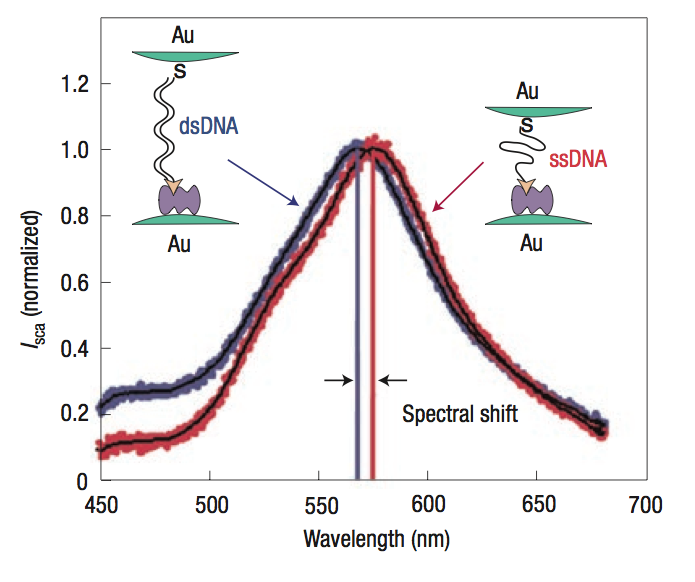
\includegraphics[width=8cm]{img/biosensingDNA.png}}
\caption{Пример спектрального сдвига в системе из двух золотых наночастиц, соединенных между собой одноцепочечной молекулой ДНК (красная линия) и двухцепочечной молекулой ДНК (синяя линия) \cite{biosensing}.}
\label{img:PR_SEM}
\end{figure}
Такие системы из двух наночастиц называются димерами. Оптическими свойствами димеров можно управлять, изменяя форму наночастиц в димере, их взаиморасположение, поляризацию падающего электромагнитного излучения.

Одними из первых димеров исследовались системы из двух нанодисков. В статье \cite{plasonrulereq} исследуется зависимость локального плазмонного резонанса от расстояния между двумя нанодисками из золота. Пары нанодисков из золота располагались на кварцевой подложке и имели толщину 25 нм и диаметр 88 нм. Расстояние между нанодисками варьировалось и составляло 212, 27, 17, 12, 7 и 2 нм. Изображение ансамбля из спаренных нанодисков с расстоянием между нанодисками 12 нм, полученное с помощью растрового электронного микроскопа, показано на рис. \ref{img:PR_SEM}.
\begin{figure}
\center{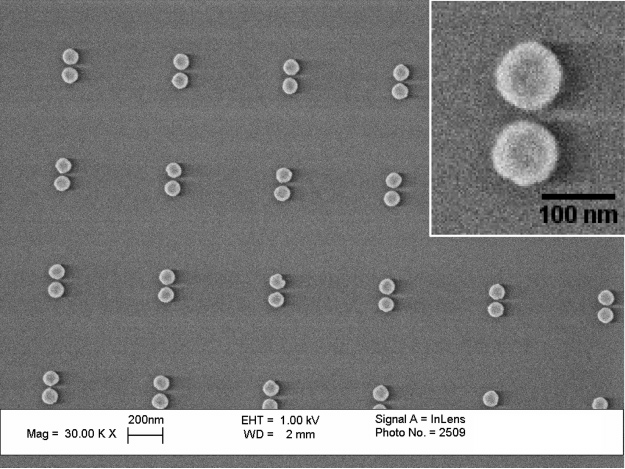
\includegraphics[width=10cm]{img/PR_SEM.png}}
\caption{Изображение пар нанодисков из золота, полученное с помощью растрового электронного микроскопа. Расстояние между нанодисками составляет 12 нм, диаметр нанодиска составляет 88 нм, а толщина --- 25 нм \cite{plasonrulereq}.}
\label{img:PR_SEM}
\end{figure}
Спектры резонансов ЛПП были получены с помощью микроспектроскопии пропускания. При падении света с поляризацией, параллельной оси между центрами нанодисков, наблюдался сдвиг резонанса ЛПП в красную область спектра при уменьшении расстояния между нанодисками. На рис.~\ref{img:PR_extinction} показана зависимость коэффициента экстинкции от длины волны падающего света с поляризацией, параллельной оси между центрами нанодисков, для различных расстояний между нанодисками.
\begin{figure}[t]
\center{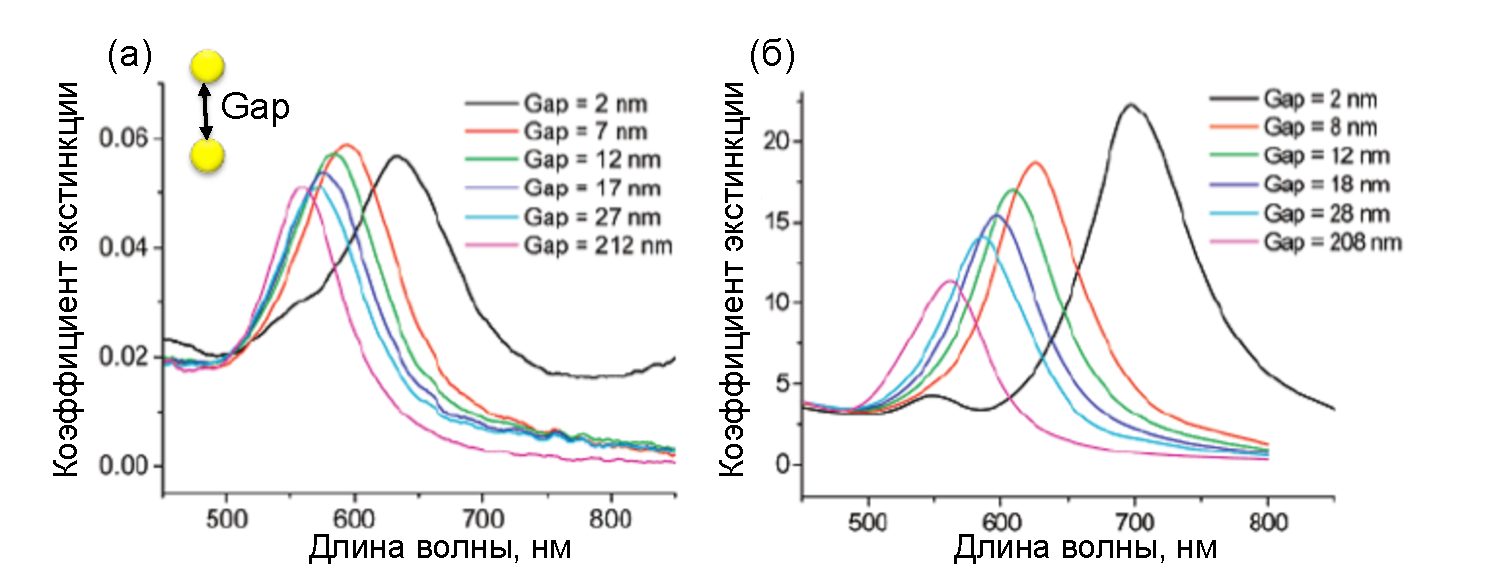
\includegraphics[width=18cm]{img/PR_extinction_ru.pdf}}
\caption{(а) Экспериментальные и (б) численные спектры коэффициента экстинкции при падении света на структуру из спаренных нанодисков из золота с различными расстояниями между нанодисками. Поляризация параллельна оси между центрами нанодисков \cite{plasonrulereq}.}
\label{img:PR_extinction}
\end{figure}
\begin{figure}[t]
\center{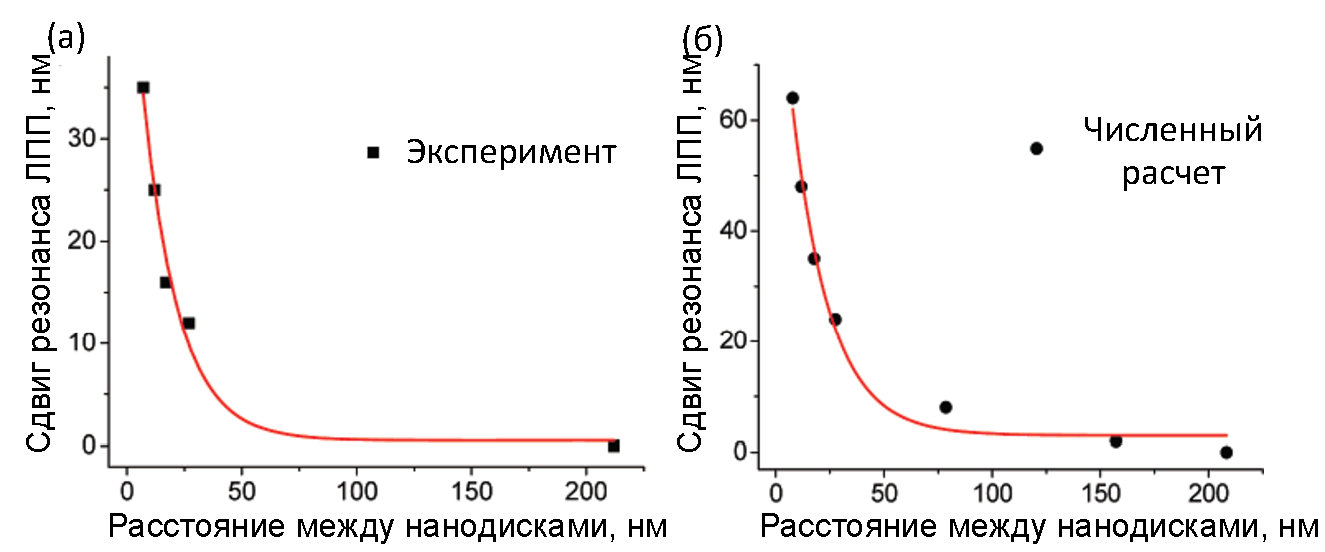
\includegraphics[width=17cm]{img/PR_ruler_ru.pdf}}
\caption{Зависимость сдвига резонанса ЛПП для пар золотых нанодисков от расстояния между нанодисками в эксперименте (а) и численных расчетах (б). Красная линия соответствует кривой $ y = y_0 + a \cdot e^{-x/l} $  \cite{plasonrulereq}.}
\label{img:PR_ruler}
\end{figure}

На рис.~\ref{img:PR_ruler} показана зависимость сдвига резонанса ЛПП от расстояния между нанодисками. Резонанс ЛПП при расстоянии между нанодисками 212 нм был выбран опорным при расчете относительного сдвига, так как взаимодействие между нанодисками можно положить минимальным.

Учитывая данное поведение системы, было выведено следующее феноменологическое уравнение для <<плазмонной линейки>>:
\begin{equation}
\frac{\Delta \lambda}{\lambda_0} \approx 0.18 \cdot \exp \left( \frac{-(s/D)}{0.23} \right),
\label{eq:plasmon_ruler}
\end{equation}
где $ \Delta \lambda $ -- величина сдвига резонанса ЛПП, $ \lambda_0 $ -- резонанс ЛПП изолированной наночастицы, $ D $ -- диаметр наночастицы. Такая линейка, например, была использована для измерения длин молекул ДНК \cite{bioplasmonruler3}.

% Далее описать взаимодействие между димерами наностержней
Димеры из золотых наностержней являются наиболее часто используемыми при исследовании оптических свойств димеров золотых наночастиц [ref: nanorod dimers]. Это связано с тем, что появляется возможность исследовать не только зависимость положения резонанса ЛПП от расстояния между наночастицами, но и изучить поведение резонанса ЛПП при различном взаимном расположении наностержней.

%%% TO-DO
% Посмотреть статьи про наностержни, взять то, что релевантно, не переборщить с картинками
% !Возможно найти некую сводную статью по всем данные о plasmon ruler
% pi димеры и sigma димеры
% написать про темные и светлые моды
% END OF TODO

\section{Описание взаимодействия спаренных наночастиц в дипольном приближении}

В данном параграфе будет рассмотрено ближнепольное взаимодействие двух золотых наностержней в дипольном приближении и продемонстрировано явление смещения резонанса ЛПП при изменении расстояния между наностержнями.
При падении периодического электромагнитного излучения на наночастицу в ней наводится дипольный момент. Тогда взаимодействие двух наночастиц можно представить как взаимодействие двух точечных диполей. Теоретическое описание взаимодействия таких диполей приведено в статье \cite{dipoleInteraction}.

Пусть один из двух диполей находится в начале декартовой системы координат (диполь (1)), а второй диполь находится на расстоянии $ r $ от первого вдоль оси $ Oz $. Энергия взаимодействия возникает вследствие взаимной поляризации, которая вычисляется следующим образом.

Пусть мгновенная поляризация диполя (1) задается следующим выражением:
\begin{equation}
\textbf{P} (1, t) = \textbf{P} \exp (-\imath \omega t),
\label{eq:instdipole1}
\end{equation}
где $ \omega $ --- частота внешнего электромагнитного поля.
Тогда векторный потенциал $ \textbf{A} $ и скалярный потенциал $ \phi $ в произвольной точке на расстоянии $ r $ от диполя определяются формулами

\begin{equation}
\textbf{A}(r, t) = - \frac{\imath \omega}{c} \textbf{P} \exp (-\imath \omega t) \frac{\exp (\imath \omega r / c)}{r},
\label{eq:vectorpotential}
\end{equation}
и
\begin{equation}
\phi(r, t) = \frac{\textbf{P} \cdot \textbf{r}}{r^2} \left( \frac{1}{r} - \frac{\imath \omega}{c} \right) \exp (-\imath \omega t) \exp (\imath \omega r / c),
\label{eq:scalarpotential}
\end{equation}
где $ c $ --- скорость света в вакууме. Соответствующее электрическое поля задается выражением:
\begin{equation}
\textbf{E} (r, t) = - \frac{1}{c} \dfrac{\partial \textbf{A}}{\partial t} - \nabla \phi.
\label{eq:elecdipolefromvector}
\end{equation}
Следовательно, получим $ \textbf{E}(r, t) = \textbf{E} (r) \exp(- \imath \omega t) $, где:

\begin{equation}
\textbf{E} = \frac{\textbf{P}}{r} \left( \frac{\omega ^2}{c^2} + \frac{\imath \omega}{c r} - \frac{1}{r^2} \right) \exp(\imath \omega r/c) - (\textbf{P} \cdot \textbf{r}) \frac{\textbf{r}}{r^3} \left( \frac{\omega ^2}{c^2} + \frac{3 \imath \omega}{c r} - \frac{3}{r^2} \right) \exp(\imath \omega r/c).
\label{eq:elecdipole}
\end{equation}
Значит, если $ \vert \textbf{r} \vert $ --- расстояние между диполями, а $ \textbf{r} $ --- направление вдоль оси $ Oz $, то компоненты $ \textbf{E}(1) $, вызванные диполем (1) при положении диполя (2), выражаются следующими формулами:

\begin{equation}
E_x (1) = f(r) P_x (1), \quad
E_y (1) = f(r) P_y (1), \quad
E_z (1) = h(r) P_z (1),
\label{eq:fieldcertesian}
\end{equation}
где
\begin{equation}
f(r) = \frac{\exp (\imath \omega r /c)}{r} \left( \frac{\omega ^2}{c^2} + \frac{\imath \omega}{c r} - \frac{1}{r^2} \right), \quad
h(r) = \frac{2 \exp (\imath \omega r /c)}{r} \left( \frac{1}{r^2} - \frac{\imath \omega}{c r} \right).
\label{eq:hf_functions}
\end{equation}
Это поле поляризует диполь (2), поляризация которого равна:
\begin{equation}
\textbf{P}(2) = \widehat{\alpha}(2) \textbf{E}(1),
\label{eq:polar2to1}
\end{equation}
где $ \widehat{\alpha} (2) $ -- тензор поляризуемости второго диполя. Эта индуцированная поляризация в свою очередь создает электрическое поле в первом диполе, наводя свою поляризацию, и в соответствии с формулой (\ref{eq:polar2to1}) получим:
\begin{equation}
\textbf{P}(1) = \widehat{\alpha}(1) \textbf{E}(2).
\label{eq:polar1to2}
\end{equation}
Из формул (\ref{eq:fieldcertesian}), (\ref{eq:polar2to1}) и (\ref{eq:polar1to2}) получим:
\begin{equation}
\textbf{P}(2) = \widehat{X}(2) \textbf{P}(1), \quad 
\textbf{P}(1) = \widehat{X}(1) \textbf{P}(2),
\label{eq:polarity}
\end{equation}
где матрицы $ \widehat{X} $ определяются следующим образом:
\begin{equation}
\widehat{X} = \left(
\begin{matrix}
\alpha _{11} f & \alpha _{12} f & \alpha _{13} h \\
\alpha _{21} f & \alpha _{22} f & \alpha _{23} h \\
\alpha _{31} f & \alpha _{31} f & \alpha _{33} h \\
\end{matrix}
\right),
\label{eq:Xmatrix}
\end{equation}
и $ \alpha _{ij} $ являются матричными элементами тензоров поляризуемости $ \widehat{\alpha}(1) $ и $ \widehat{\alpha}(2) $, соответственно. Уравнения (\ref{eq:polarity}) обеспечивают условие согласования на разрешенные моды:
\begin{equation}
\textbf{P}(1) = \widehat{Y} \textbf{P}(1), \quad
\widehat{Y} = \widehat{X}(1) \widehat{X}(2).
\label{eq:allowedmodes}
\end{equation}
Частоты разрешенных мод задаются дисперсионным соотношением:
\begin{equation}
D(\omega) \equiv \det (\widehat{I} - \widehat{Y}) = 0.
\label{eq:dispersiondipole}
\end{equation}

Из уравнений (\ref{eq:Xmatrix}) и (\ref{eq:allowedmodes}) компоненты матрицы $ \widehat{Y} $ имеют вид:
\begin{subequations}
\begin{gather}
y_{11} = \{\alpha_{11}(1) \alpha_{11}(2) + \alpha_{12}(1) \alpha_{21}(2)  \} f^2 + \alpha_{13}(1) \alpha_{31}(2) fh , \label{eq:y11} \\
y_{22} = \{\alpha_{21}(1) \alpha_{12}(2) + \alpha_{22}(1) \alpha_{22}(2)  \} f^2 + \alpha_{23}(1) \alpha_{32}(2) fh , \label{eq:y22} \\
y_{33} = \{\alpha_{31}(1) \alpha_{13}(2) + \alpha_{32}(1) \alpha_{23}(2)  \} fh + \alpha_{33}(1) \alpha_{33}(2) h^2 , \label{eq:y33} \\
y_{12} = \{\alpha_{11}(1) \alpha_{12}(2) + \alpha_{12}(1) \alpha_{22}(2)  \} f^2 + \alpha_{13}(1) \alpha_{32}(2) fh , \label{eq:y12} \\
y_{13} = \{\alpha_{11}(1) \alpha_{13}(2) + \alpha_{12}(1) \alpha_{23}(2)  \} fh + \alpha_{13}(1) \alpha_{33}(2) h^2 , \label{eq:y13} \\
y_{23} = \{\alpha_{21}(1) \alpha_{13}(2) + \alpha_{22}(1) \alpha_{23}(2)  \} fh + \alpha_{23}(1) \alpha_{33}(2) h^2 . \label{eq:y23}
\end{gather}
\end{subequations}
Матричные элементы $ y_{21} $, $ y_{31} $ и $ y_{32} $ получаются из уравнений (\ref{eq:y12}), (\ref{eq:y13}) и (\ref{eq:y23}) путем перестановки индексов 1 и 2 диполей. Например, $ y_{21} = y_{12} \{ (1) \rightleftarrows (2) \} $. 

Возьмем модель двух взаимодействующих золотых эллипсоидов. Тогда тензор поляризуемости будет анизотропным. Пусть $ \alpha = \alpha_{xx} = \alpha_{11} \neq 0 $, а остальные компоненты равны нулю, что соответствует состоянию, в котором резонансная частота, возбужденная электрическим полем вдоль оси $ Ox $, находится вдали от других резонансных частот. Тогда матрица (\ref{eq:Xmatrix}) преобразуется в матрицу:
\begin{equation}
\widehat{X} = \left(
\begin{matrix}
\alpha f & 0 & 0 \\
0 & 0 & 0 \\
0 & 0 & 0 \\
\end{matrix}
\right).
\label{eq:Xmatrix_dipole}
\end{equation}

Используя уравнение (\ref{eq:polarizabilityEllip}) для поляризуемости эллипсоида и подставляя формулу Друде (\ref{eq:EpsilonFreeElectron}) для диэлектрической проницаемости металла, получим уравнение поляризуемости:
\begin{equation}
\alpha = \frac{\omega_p^2}{\omega_p^2 - \omega ^2 / L_x} \frac{V}{4 \pi},
\label{eq:polarizability_dipole}
\end{equation}
где $ \omega_p $ -- плазменная частота металла, $ L_x $ -- фактор деполяризации эллипсоида, определяемый формулой (\ref{eq:Lfactor}), $ V $ -- объем эллипсоида. Дисперсионное соотношение (\ref{eq:dispersiondipole}) преобразуется к виду:
\begin{equation}
\alpha f = \pm 1.
\label{eq:dispersion_dipole}
\end{equation}
Рассмотрим ближнепольный случай, для которого $ r \ll \lambda $. Тогда множитель $ \exp (\imath k r) $ функции $ f(r) $, где $ k = \omega / c $, можно разложить в ряд Тейлора. Тогда для функции $ f(r) $ получим уравнение:
\begin{equation}
f(r) = \frac{\exp (\imath k r)}{r} \left( k^2 + \frac{\imath k}{r} - \frac{1}{r^2} \right) \simeq \frac{1}{r} \left( 1 + \imath k r - \frac{k^2 r^2}{2} + ... \right) \left( k^2 + \frac{\imath k}{r} - \frac{1}{r^2} \right).
\label{eq:f_Taylor}
\end{equation}
Так как $ k r \ll 1 $, то $ \frac{1}{(kr)^2} \gg \frac{1}{kr} $ и $ \frac{1}{(kr)^3} \gg \frac{1}{kr} $ и пренебрегая членами порядка $ r^n $, где $ n \geq -1 $, получим:
\begin{equation}
f(r) \simeq - \frac{1}{r^3}.
\label{eq:f_dipole}
\end{equation}
Подставляя (\ref{eq:f_dipole}) в (\ref{eq:dispersion_dipole}), получим уравнение для собственных частот:
\begin{equation}
\omega_{\pm} = \omega_p \sqrt{L_x} \sqrt{1 \mp \frac{V}{4 \pi r^3}}.
\label{eq:freq_dipole}
\end{equation}
Выражая уравнение (\ref{eq:freq_dipole}) в длинах волн, получим:
\begin{equation}
\lambda_{\pm} = \frac{\lambda_p}{\sqrt{L_x}} \frac{1}{\sqrt{1 \mp V / 4 \pi r^3}},
\label{eq:wl_dipole}
\end{equation}
где $ \lambda_p $ -- плазменная длина волны.

Рассмотрим два эллипсоида, у которых длины полуосей равны 75 нм вдоль оси $ Ox $,  15 нм вдоль оси $ Oy $ и 25 нм вдоль оси $ Oz $.  Для таких эллипсоидов фактор деполяризации вдоль оси $ Ox $ $ L_x \approx 0.08  $. Объем одного эллипсоида $ V \approx 1.18*10^5 $ нм$ ^3 $. Взаимное расположение этих 
эллипсоидов показано на рис.~\ref{img:semianalytical_dd}a. Значение плазменной частоты $ f_p = \omega_p / 2 \pi $ взято из статьи \cite{plasma_freq} и составляет $ 2.183*10^{15} $ Гц.

\begin{figure}[h]
\center{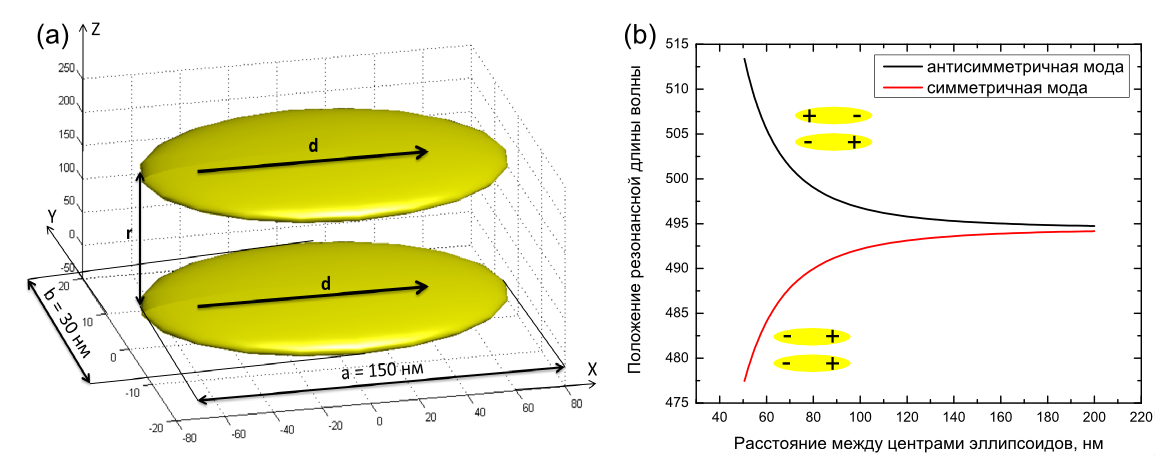
\includegraphics[width=16cm]{img/fenomenology.png}}
\caption{Взаимное расположение двух эллипсоидов из золота и направление дипольного момента $ \textbf{d} $ (а), зависимость резонансной длины волны от расстояния $ r $ между центрами эллипсоидов (b).}
\label{img:semianalytical_dd}
\end{figure}

Зависимость резонансной длины волны от расстояния между центрами эллипсоидов показано на рис.~\ref{img:semianalytical_dd}b. На больших расстояниях взаимодействия между частицами нет, поэтому каждую частицу можно предположить одиночной, с собственной резонансной длиной волны $ \lambda_{isolated} \approx  495 $ нм. При взаимодействии двух частиц появляется расщепление на две моды: симметричную с большей энергией взаимодействия и антисимметричную с меньшей энергией взаимодействия. При расстояниях $ r \ll \lambda $ в однородных внешних полях антисимметричная мода возбуждается неэффективно, поэтому больший интерес представляет симметричная мода, на которой построены принципы <<плазмонной  линейки>>. Мгновенное распределение зарядов в симметричном  и антисимметричном случае показано на рис.~\ref{img:semianalytical_dd}b. 
\section{Метод конечных разностей во временной области}

Для расчетов спектра пропускания и локального распределения плотности мощности электромагнитного поля димеров плазмонных наночастиц часто используют метод конечных разностей во временной области. Метод конечных разностей во временной области (англ. Finite Difference Time Domain, FDTD) — один из наиболее популярных методов численной электродинамики, основанный на дискретизации уравнений Максвелла, записанных в дифференциальной форме. Рассмотрим базовый алгоритм Йи для численного решения уравнений Максвелла, первоначально использованный в методе FDTD и подробно изложенный в статье~\cite{FDTDYee}.

Уравнения Максвелла в изотропной среде в системе СИ имеют вид:
\begin{subequations}
\begin{gather}
\dfrac{\partial \textbf{B}}{\partial t} + \nabla \times \textbf{E} = 0, \label{eq:MaxwellA} \\
- \dfrac{\partial \textbf{D}}{\partial t} + \nabla \times \textbf{H} = \textbf{J}, \label{eq:MaxwellB} \\
\nabla \cdot \textbf{D} = \rho \label{eq:MaxwellC}, \\
\nabla \cdot \textbf{B} = 0 \label{eq:MaxwellD}.
\end{gather}
\end{subequations}

В декартовых координатах уравнения~(\ref{eq:MaxwellA}) и~(\ref{eq:MaxwellB}) эквивалентны следующей системе скалярных уравнений:

\begin{subequations}
\begin{gather}
- \dfrac{\partial B_x}{\partial t} = \dfrac{\partial E_z}{\partial y} - \dfrac{\partial E_y}{\partial z} \label{eq:scalarMEa}, \\
- \dfrac{\partial B_y}{\partial t} = \dfrac{\partial E_x}{\partial z} - \dfrac{\partial E_z}{\partial x} \label{eq:scalarMEb}, \\
\dfrac{\partial B_z}{\partial t} = \dfrac{\partial E_x}{\partial y} - \dfrac{\partial E_y}{\partial x} \label{eq:scalarMEc}, \\
- \dfrac{\partial D_x}{\partial t} = \dfrac{\partial H_z}{\partial y} - \dfrac{\partial H_y}{\partial z}+J_x \label{eq:scalarMEd}, \\
- \dfrac{\partial D_y}{\partial t} = \dfrac{\partial H_x}{\partial z} - \dfrac{\partial H_z}{\partial x}+J_y \label{eq:scalarMEe}, \\
- \dfrac{\partial D_z}{\partial t} = \dfrac{\partial H_y}{\partial x} - \dfrac{\partial H_x}{\partial y}+J_z \label{eq:scalarMEf}.
\end{gather}
\end{subequations}
Вводя разностную сетку, для точки в пространстве получим:
\begin{equation}
(i, j, k) = (i \Delta x, j \Delta y, k \Delta z),
\label{eq:pointgrid}
\end{equation}
и для любой функции координат и времени положим:
\begin{equation}
F(i \Delta x, j \Delta y, k \Delta z, n \Delta t ) = F^n (i, j, k).
\label{eq:funcgrid}
\end{equation}

При идеально проводящих граничных условиях система разностных уравнений~(\ref{eq:scalarMEa})~--~(\ref{eq:scalarMEf}) выглядит следующим образом. Для~(\ref{eq:scalarMEa}):

\begin{multline}
\dfrac{B_{x} ^{n + 1/2}(i, j + \frac{1}{2}, k + \frac{1}{2}) - B_{x} ^{n - 1/2}(i, j + \frac{1}{2}, k + \frac{1}{2}) }{\Delta t}  =\\
= \dfrac{E_{y} ^{n} (i, j + \frac{1}{2}, k + 1) - E_{y} ^{n} (i, j + \frac{1}{2}, k)}{\Delta z} - \\
- \dfrac{E_{z} ^{n} (i, j + 1, k + \frac{1}{2}) - E_{z} ^{n} (i, j, k + \frac{1}{2})}{\Delta y}.
\label{eq:gridScalarA}
\end{multline}
Разностные уравнения для~(\ref{eq:scalarMEb}) и~(\ref{eq:scalarMEc}) выглядят аналогично~(\ref{eq:scalarMEa}).

Для~(\ref{eq:scalarMEd}) получим:
\begin{multline}
- \dfrac{D_{x} ^{n}(i + \frac{1}{2}, j, k) - D_{x} ^{n-1}(i + \frac{1}{2}, j, k) }{\Delta t} = \dfrac{H_{z} ^{n - 1/2} (i + \frac{1}{2}, j + \frac{1}{2}, k) - H_{y} ^{n - 1/2} (i + \frac{1}{2}, j - \frac{1}{2}, k)}{\Delta y} - \\
- \dfrac{H_{y} ^{n - 1/2} (i + \frac{1}{2}, j, k + \frac{1}{2}) - H_{z} ^{n - 1/2} (i + \frac{1}{2}, j, k - \frac{1}{2})}{\Delta z} + J_{x} ^{n - 1/2} (i + 1/2, j, k).
\label{eq:gridScalarD}
\end{multline}
Разностные уравнения, относящиеся к~(\ref{eq:scalarMEe}) и~(\ref{eq:scalarMEf}), получаются аналогичным путем. Получается, что сетки для полей $ E $ и $ H $ смещены по отношению друг к другу на половину шага дискретизации по времени и по каждой из пространственных переменных. Конечно-разностные уравнения позволяют определить поля $ E $ и $ H $ на данном временном шаге на основании известных значений полей на предыдущем, как показано на рис.\ref{img:FDTDGrid}. При заданных начальных условиях алгоритм Йи дает эволюционирующее  во времени решение во времени от начала отсчета с заданным временным шагом.

\begin{figure}[h]
\center{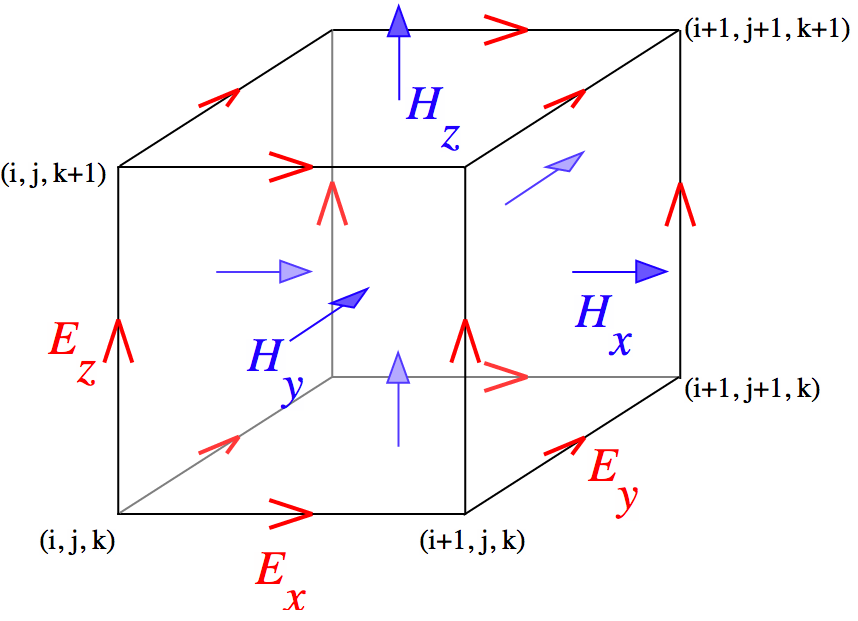
\includegraphics[width=8cm]{img/FDTDGrid.png}}
\caption{Поля в ячейке сетки FDTD. $ E $ компонента находится в середине ребер сетки, а $ H $ компонента -- в середине граней\cite{FDTDYee}.}
\label{img:FDTDGrid}
\end{figure}

Как и в любом другом разностном методе, в FDTD существует проблема неточного отображения границы тела на вычислительную сетку. Любая кривая поверхность, разделяющая соседние среды и геометрически не согласованная с сеткой, будет искажаться эффектом «лестничного приближения». Для решения данной проблемы можно использовать дополнительную сетку с большим разрешением в тех областях пространства, где расположены тела со сложной геометрической структурой.

Для того, чтобы ограничить объем сетки, в FDTD нужны особые поглощающие граничные условия, которые моделируют уход электромагнитной волны на бесконечность. Для этого используются поглощающие граничные условия Мура или Ляо, или идеально согласованные слои (Perfectly Matched Layers, PML). Условия Мура или Ляо намного проще, чем PML. Тем не менее, PML — строго говоря, являющиеся поглощающей приграничной областью, а не граничным условием как таковым — позволяют получить на порядки меньшие по величине коэффициенты отражения от границы.
\section{Методика изготовления нанодимеров}

На данный момент существует достаточно много способов изготовления планарных наноструктур различных размеров и форм, и наиболее распространенными являются различные виды литографии \cite{nanotechnologybook}. В этом методе изображение элемента или схемы выполняется в виде рисунка на металлической пленке, нанесенной на прозрачную подложку. Такой рисунок называется маской или шаблоном. Затем рисунок с помощью потока электронов переносится на полупроводниковую пластину, в которой слой за слоем формируется физическая структура требуемого объекта. Таким образом, литография -- процесс переноса изображения с маски на подложку. Для этого на поверхности подложки создается пленочное покрытие из полимерного материала -- резиста; покрытие облучают через маску с изображением элементов схемы и затем покрытие проявляют (травят в растворителе) так, что изображение схемы переносится на подложку.

Существует два основных вида резистов: позитивные и негативные. Если в результате облучения резист полимеризуется и теряет растворимость, то обработка растворителем (проявление) ведет к удалению только необлученных участков и на подложке возникает негативное изображение маски. Соответствующие резисты называются негативными. Если же в результате воздействия облучения резист становится растворимым, то при облучении через маску и последующим проявлении удаляются облученные участки и на подложке возникает позитивное изображение маски. Такие резисты называются позитивными. На рис.~\ref{img:litography} слева приведен процесс проявления образца с пленкой негативного резиста, а справа -- позитивного. Далее такая структура подвергается травлению, и в результате получается массив объектов на поверхности подложки.

\begin{figure}
\center{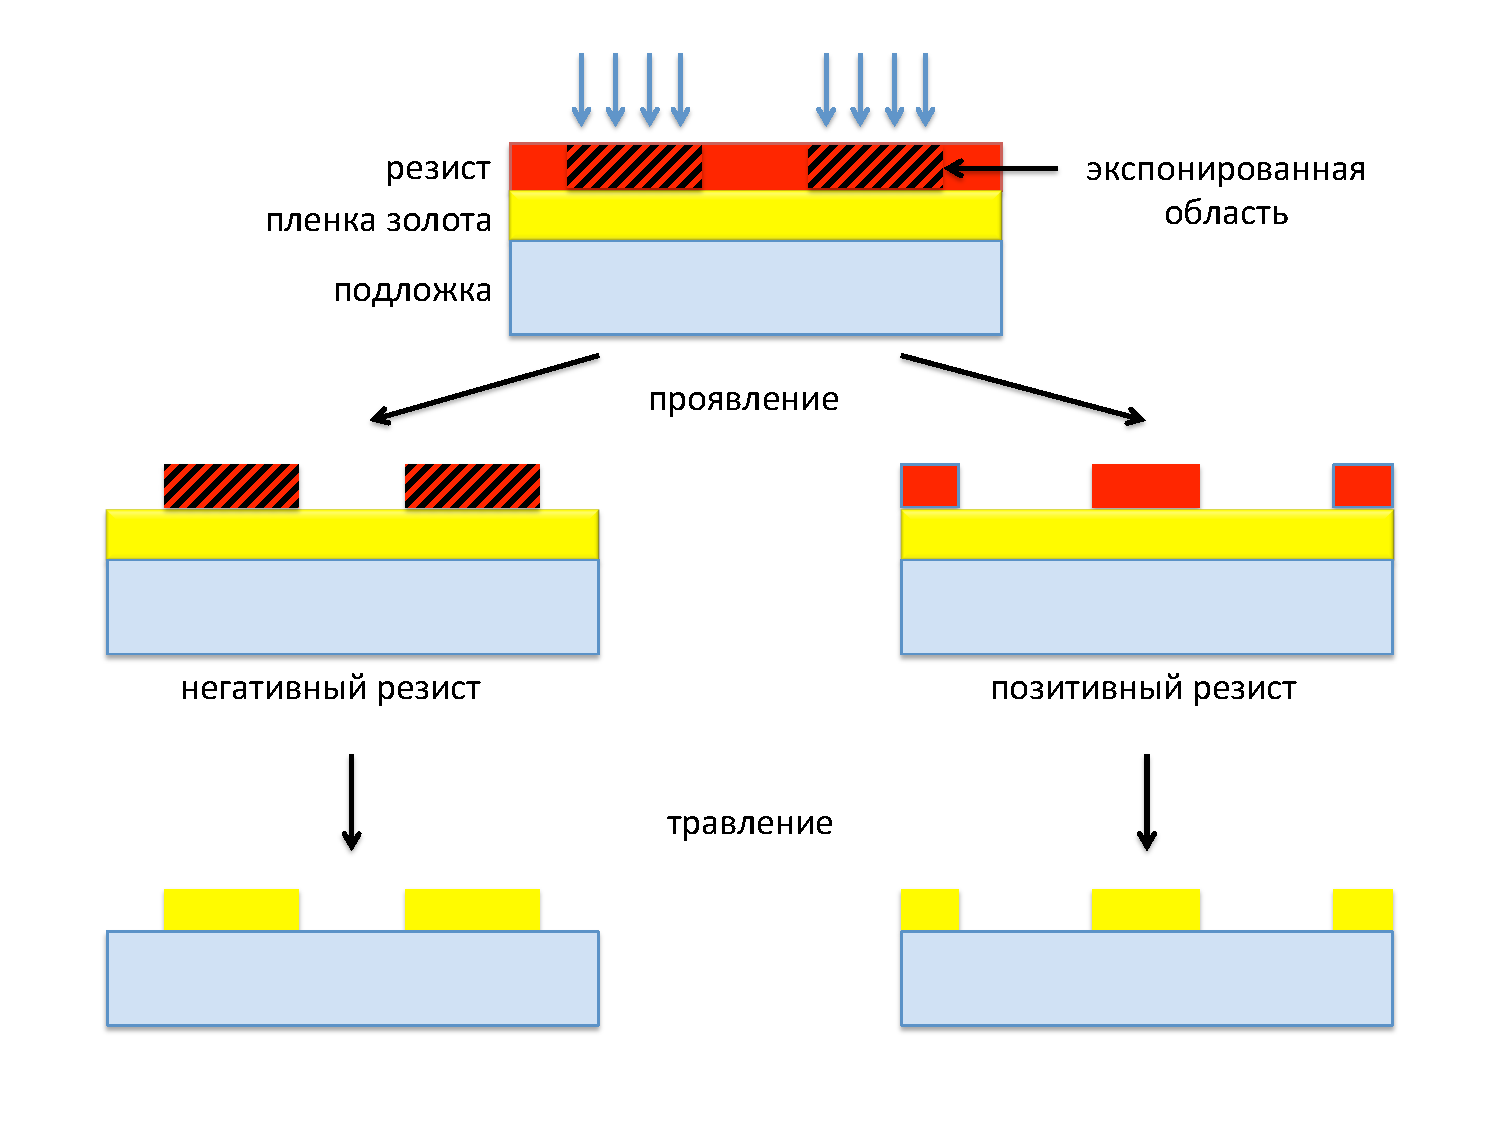
\includegraphics[width=12cm]{img/litography.pdf}}
\caption{Основные этапы литографического процесса с использованием негативного (слева) и позитивного (справа) резистов.}
\label{img:litography}
\end{figure}

Создание структур субмикронных размеров возможно с помощью электронно-лучевой литографии (ЭЛЛ) \cite{SPIEnanofabrication}, позволяющий получать объекты с характерным размером меньше 1 нм. Существуют две системы ЭЛЛ --- сканирующая и проекционная. При использовании сканирующей системы резист экспонируется фокусированным потоком электронов. В сканирующей ЭЛЛ электронный луч перемещается в плоскости рисунка и производит его последовательное экспонирование. Информация для управления электронным лучом хранится в памяти управляющего компьютера, поэтому не нужно применять какие-либо шаблоны. Однако последовательное сканирование всего рисунка приводит к значительному увеличению времени экспонирования. В проекционной системе широкий несфокусированный поток электронов можно использовать для получения всего рисунка в течение одной экспозиции. Соответствующая электронная проекционная система описана в \cite{projectelectron}. В этой системе фотокатод расположен на поверхности оптической маски с заданным рисунком. Ультрафиолетовые лучи облучают фотокатодный слой через маску, что вызывает эмиссию электронов с фотокатода в облученных местах рисунка. Эти электроны проецируются на поверхность резиста с помощью однородных электростатических и магнитных полей. В результате на всей площади подложки рисунок создается за одну экспозицию. На рис.\ref{img:EBLscheme} представлены схемы установок для сканирующей (слева) и проекционной (справа) систем ЭЛЛ. 

\begin{figure}
\center{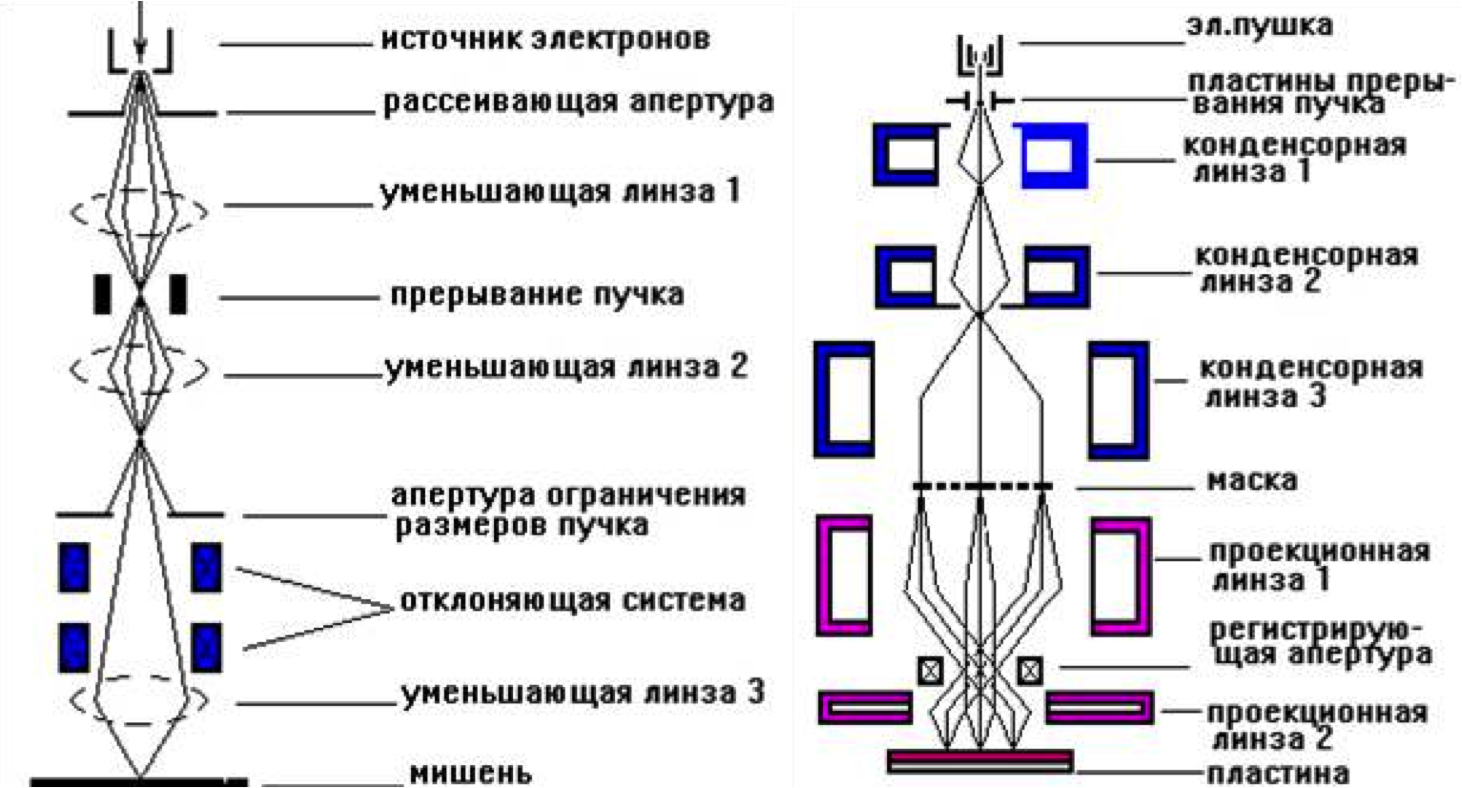
\includegraphics[width=15cm]{img/EBLschemes.png}}
\caption{Схемы установок для сканирующей (слева) и проекционной (справа) систем ЭЛЛ\cite{nanotechnologybook}.}
\label{img:EBLscheme}
\end{figure}


\section{Постановка задачи}

В результате обзора литературных источников можно сделать вывод о том, что изучение эффектов взаимодействия димеров различной геометрической формы  является актуальной на сегодняшний день задачей. Ранее систематически не исследовались резонансные особенности $ \pi $-димеров золотых наностержней, а также не исследовалось возбуждение резонансов высоких порядков в димерах наностержней.

В данной работе поставлены и решены следующие задачи:
\begin{enumerate}
\item Численное моделирование смещения резонанса локальных плазмон-поляритонов в димерах золотых наностержней различной длины и вывод уравнения плазмонной линейки для $ \pi $-димера золотых наностержней.
\item Экспериментальные обнаружение и характеризация смещения резонанса локальных плазмон-поляритонов в $ \pi $-димерах золотых наностержней, изготовленных методом электронно-лучевой литографии, сравнение теоретических и экспериментальных данных.
\item Оценка возможности использования димеров наностержней в качестве плазмонной линейки и определение диапазона расстояний, в котором плазмонная линейка может функционировать. Сравнение характеристик $ \pi $-димеров как плазмонных линеек при их работе на локальных плазмон-поляритонах первого и второго порядка.
\end{enumerate}
\newpage
\nonumchapter{Результаты}
\nonumchapter{Экспериментальные результаты}
\section{Исследуемые образцы}

В данной работе были исследованы образцы, представляющие собой пары параллельных наностержней из золота, расположенных на подложке из плавленного кварца. Ансамбли из наностержней были изготовлены с помощью  электронно-лучевой литографии коллегами из Парижского института фундаментальной электроники (Institut d'Electronique Fondamentale). Наноструктурированная поверхность с одинаковыми парами наностержней была площадью 100*100 мкм$ ^2 $.
На рис.~\ref{img:sample} схематично показано расположение ансамблей димеров наностержней. В каждом из ансамблей 2 изменяющихся параметра -- длина наностержней и расстояние между ними -- были фиксированы, расстояние между ансамблями димеров составляло 850 мкм. 
\begin{figure}[!h]
\center{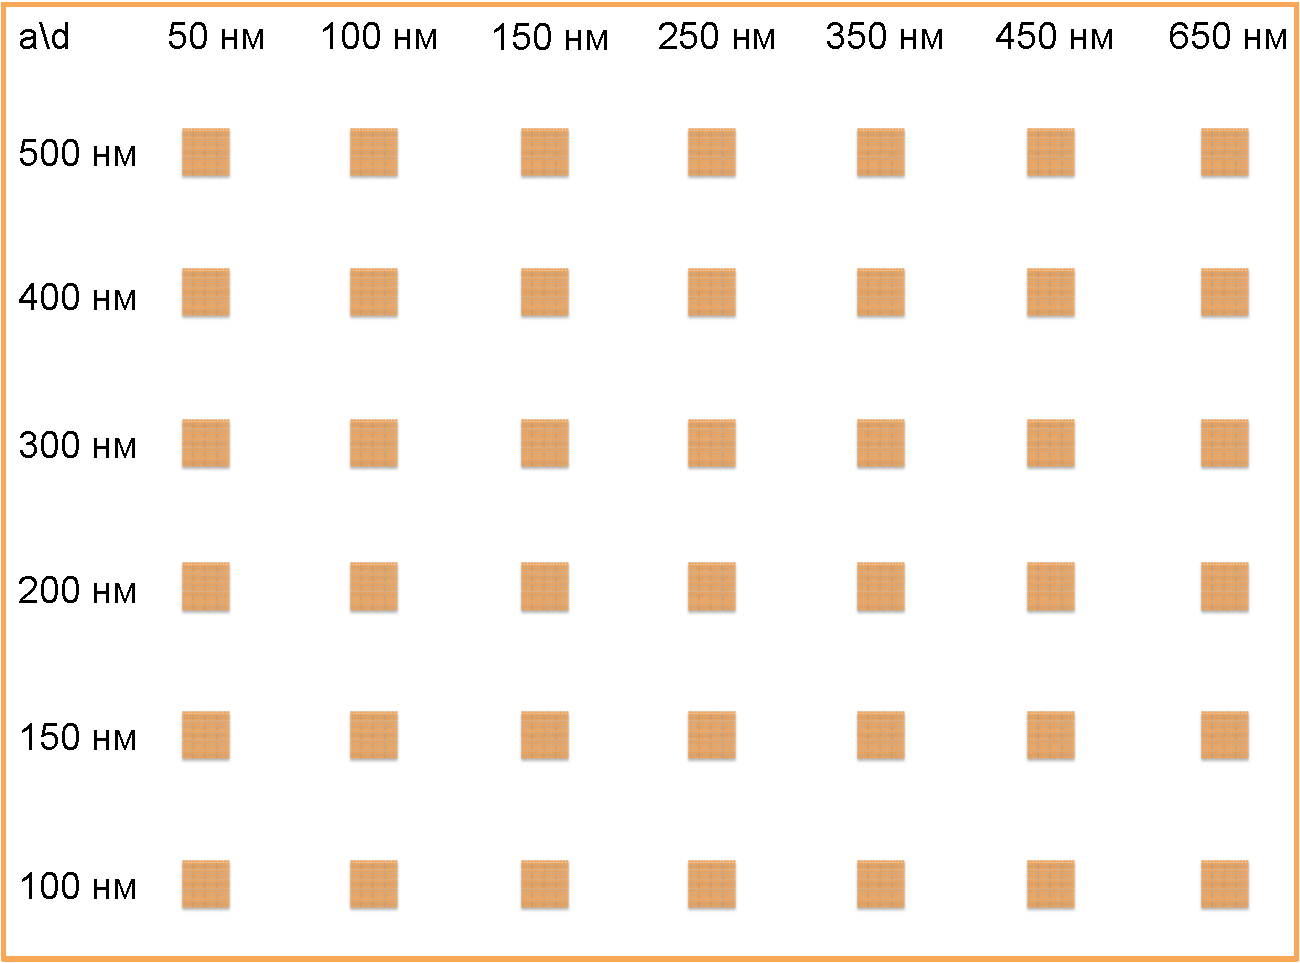
\includegraphics[width=10cm]{img/samples.pdf}}
\caption{Схематичное расположение ансамблей димеров золотых наностержней. В каждом из ансамблей фиксирована длина наностержней \textit{a} и расстояние \textit{d} между ними. Расстояние между ансамблями димеров составляет 850 нм.}
\label{img:sample}
\end{figure}

Расстояние между димерами наностержней составляет 1 мкм, чтобы обеспечить отсутствие ближнепольного взаимодействия между димерами. На рис.~\ref{img:SEMsample} показано изображение одного из ансамблей димеров, полученного с помощью растрового электронного микроскопа.
\begin{figure}[!h]
\center{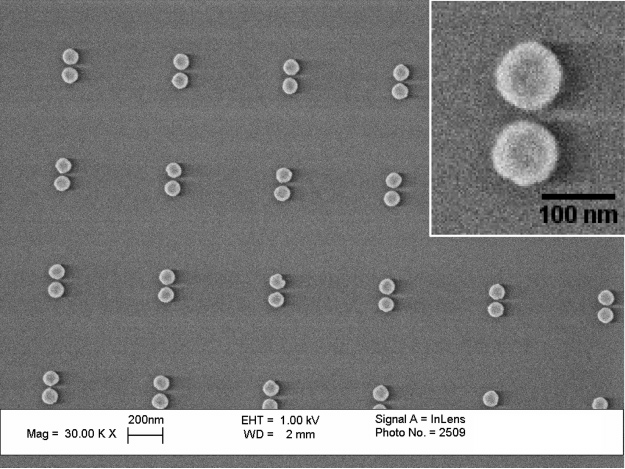
\includegraphics[width=10cm]{img/PR_SEM.png}}
\caption{Изображение одного из исследуемых ансамблей димеров из золота, полученного с помощью растрового электронного микроскопа.}
\label{img:SEMsample}
\end{figure}
В каждом ансамбле димеров все геометрические параметры димеров были одинаковые, в то время как в различных ансамблях варьировалась длина наностержней и расстояние между ними. Длина наностержней составляла $ a = $ 100, 150, 200, 400, 500 нм, а расстояние между ними -- $ d = $ 50, 100, 150, 250, 350, 450, 650 нм. По изображениям с растрового электронного микроскопа также рассчитывалась погрешность в определении средней длины и ширины наностержней, составившая не более 3 нм и 1 нм, соответственно.

%Здесь секция для комментариев
\section{Численный эксперимент}

Численный эксперимент проводился с помощью программного пакета Lumerical FDTD Solutions. При этом исследовался спектр пропускания пар наностержней в виде прямоугольных параллелепипедов. Ширина и высота наностержней оставались фиксированными во всех численных расчетах и равнялись 50 нм и 30 нм, соответственно. Вид исследуемой структуры и основные элементы для проведения численного расчета показаны на рис.~\ref{img:lumerical}. 
\begin{figure}
\center{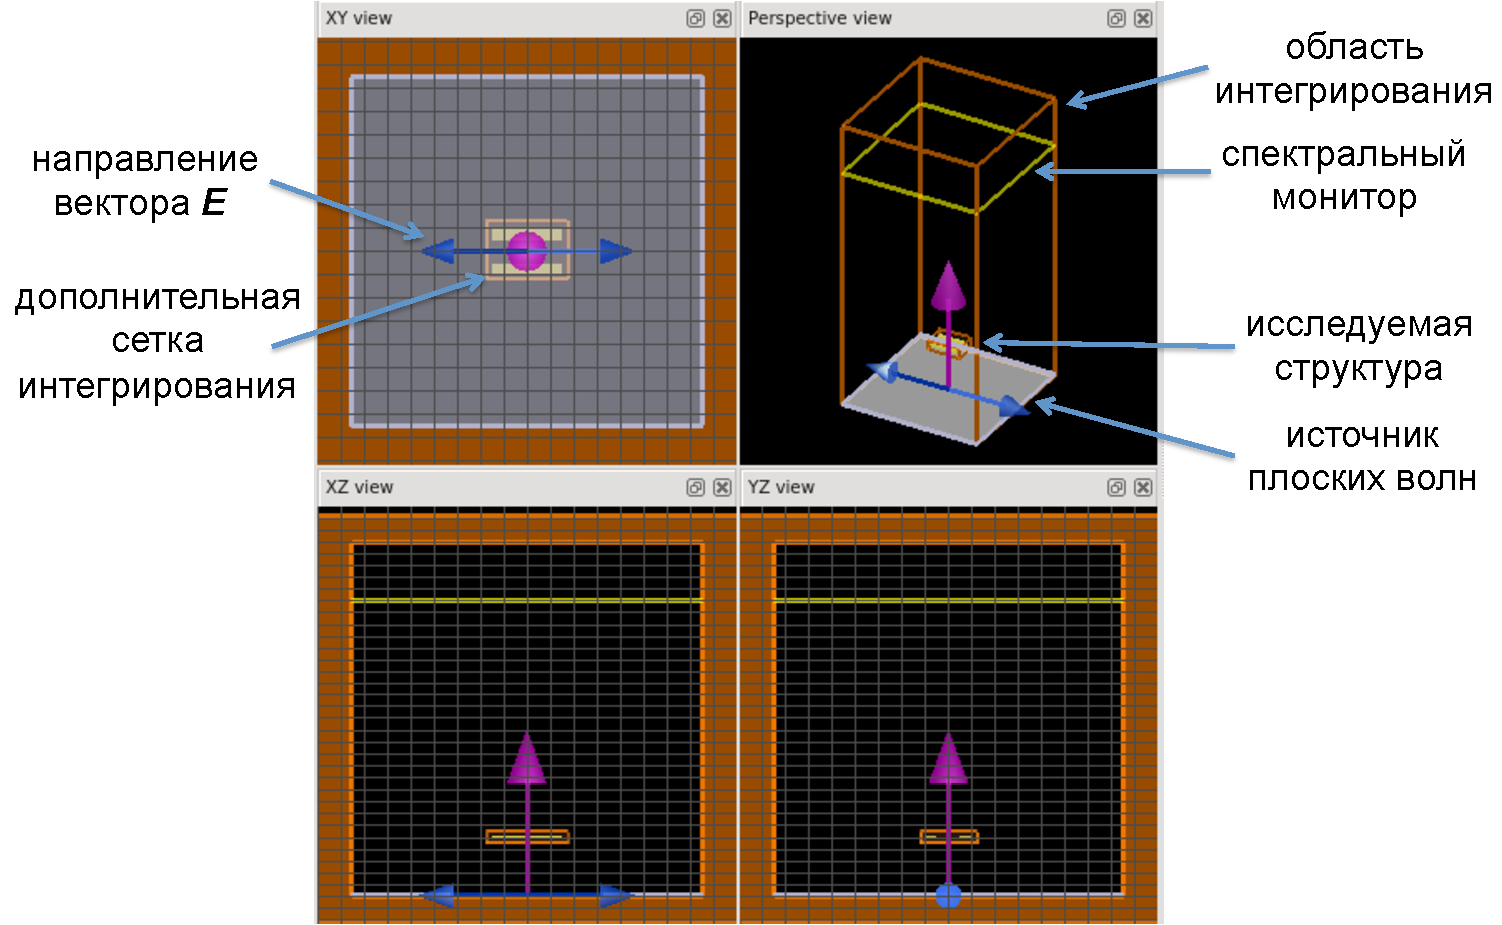
\includegraphics[width=12cm]{img/FDTD/lumerical.pdf}}
\caption{Вид исследуемой структуры и основные элементы для проведения численного расчета в программе Lumerical FDTD Solutions.}
\label{img:lumerical}
\end{figure}

Область интегрирования составляла 1.5 * 1.5 * 3 мкм$ ^3 $. Во всех пограничных плоскостях были выбраны граничные условия PML. Расчет спектра производился на расстоянии 1.5 мкм от образца для того, чтобы избежать детектирования ближнего поля. Минимальное количество узлов сетки было 22 на длину волны, которое было определено проверкой на сходимость; в дополнительной сетке расстояние между узлами сетки составляло 5 нм для улучшения точности вычислений. На образец падал фемтосекундный импульс с поляризацией, параллельной наностержням. Далее, с помощью преобразования Фурье рассчитывался спектр пропускания для различных длин волн падающего электромагнитного излучения. Характерный спектр пропускания показан на рис.~\ref{img:spectraFDTDa500d100}. Наблюдаются два резонанса: более глубокий при длине волны $ \approx 1600 $ нм  -- резонанс первого порядка, и при длине волны $ \approx 680 $ нм -- резонанс второго порядка.
\begin{figure}
\center{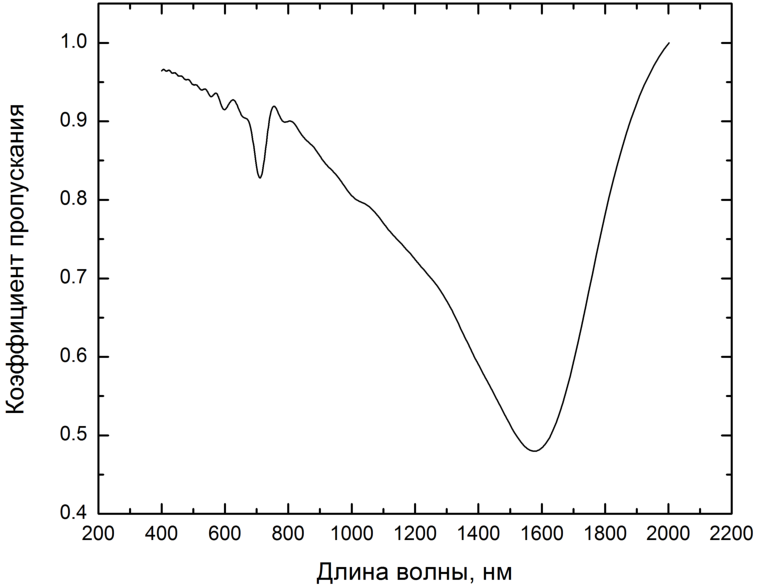
\includegraphics[width=12cm]{img/FDTD/spectra_a500d100.pdf}}
\caption{Спектр пропускания димера наностержней длиной 500 нм и расстоянием 100 нм между наностержнями, рассчитанный с помощью программного пакета Lumerical FDTD.}
\label{img:spectraFDTDa500d100}
\end{figure}

Локальное распределение плотности мощности электромагнитного поля для данных параметров пар наностержней представлено на рис.~\ref{img:locala500d100FDTD}. При этом рассчитывалось значение квадрата модуля вектора электрической напряженности $ \lvert E \rvert ^2 $ на расстоянии 20~нм от наностержней вдоль оси $ Oz $ на резонансных длинах волн. Видно, что при падении света с длиной волны 1600 нм (рис.~\ref{img:locala500d100FDTD}б) в наностержне возникает две пучности плотности мощности электромагнитного поля, а при падении света c длиной волны 680 нм (рис.~\ref{img:locala500d100FDTD}б) --- четыре пучности.

\begin{figure}
\center{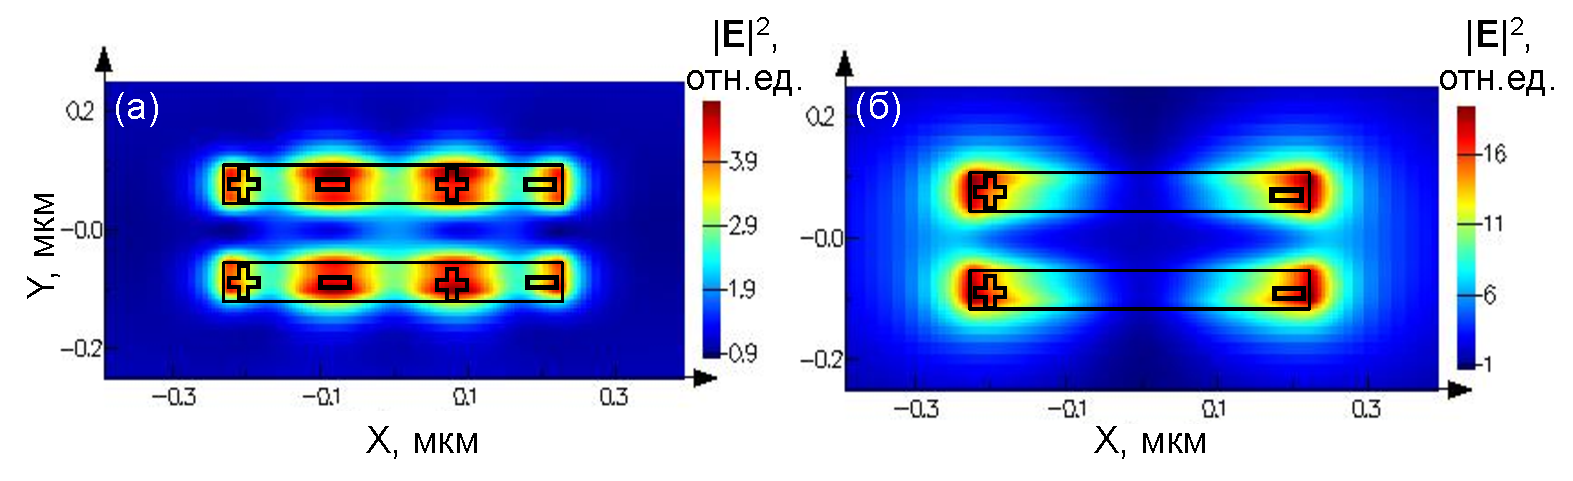
\includegraphics[width=16cm]{img/FDTD/localfield.pdf}}
\caption{Локальное распределение электромагнитного поля на расстоянии 20 нм от наностержней и мгновенное распределение зарядов при падающем электромагнитном излучении с длиной волны 680 нм (a) и 1600 нм (б).}
\label{img:locala500d100FDTD}
\end{figure}

Далее варьировалось расстояние между наностержнями фиксированной длины 500 нм от 10 нм до 650 нм с шагом 20 нм. В итоге были получены спектры пропускания для различных расстояний между наностержнями. В каждом из спектров определялись положения резонансов первого и второго порядков. Графики зависимости положения резонансов первого и второго порядков от расстояния между наностержнями представлены на рис.~\ref{img:a500PML}. На расстояниях до 150 нм график зависимости схож с графиком на рис.~\ref{img:semianalytical_dd} для случая симметричной моды. Далее начинает появляться вклад дальнепольного взаимодействия, в связи с чем кривая положения резонанса не носит монотонный характер, а появляются осцилляции. Для резонанса второго порядка кривая носит монотонный характер до $ \approx 400 $ нм, а дальше начинаются осцилляции с амплитудой $ \approx 3 $ нм. Значит, данную структуру можно использовать в качестве <<плазмонной линейки>> для резонанса первого порядка до $ \approx 150 $ нм, а для резонанса второго порядка --- до $ \approx 400 $ нм.

\begin{figure}
\center{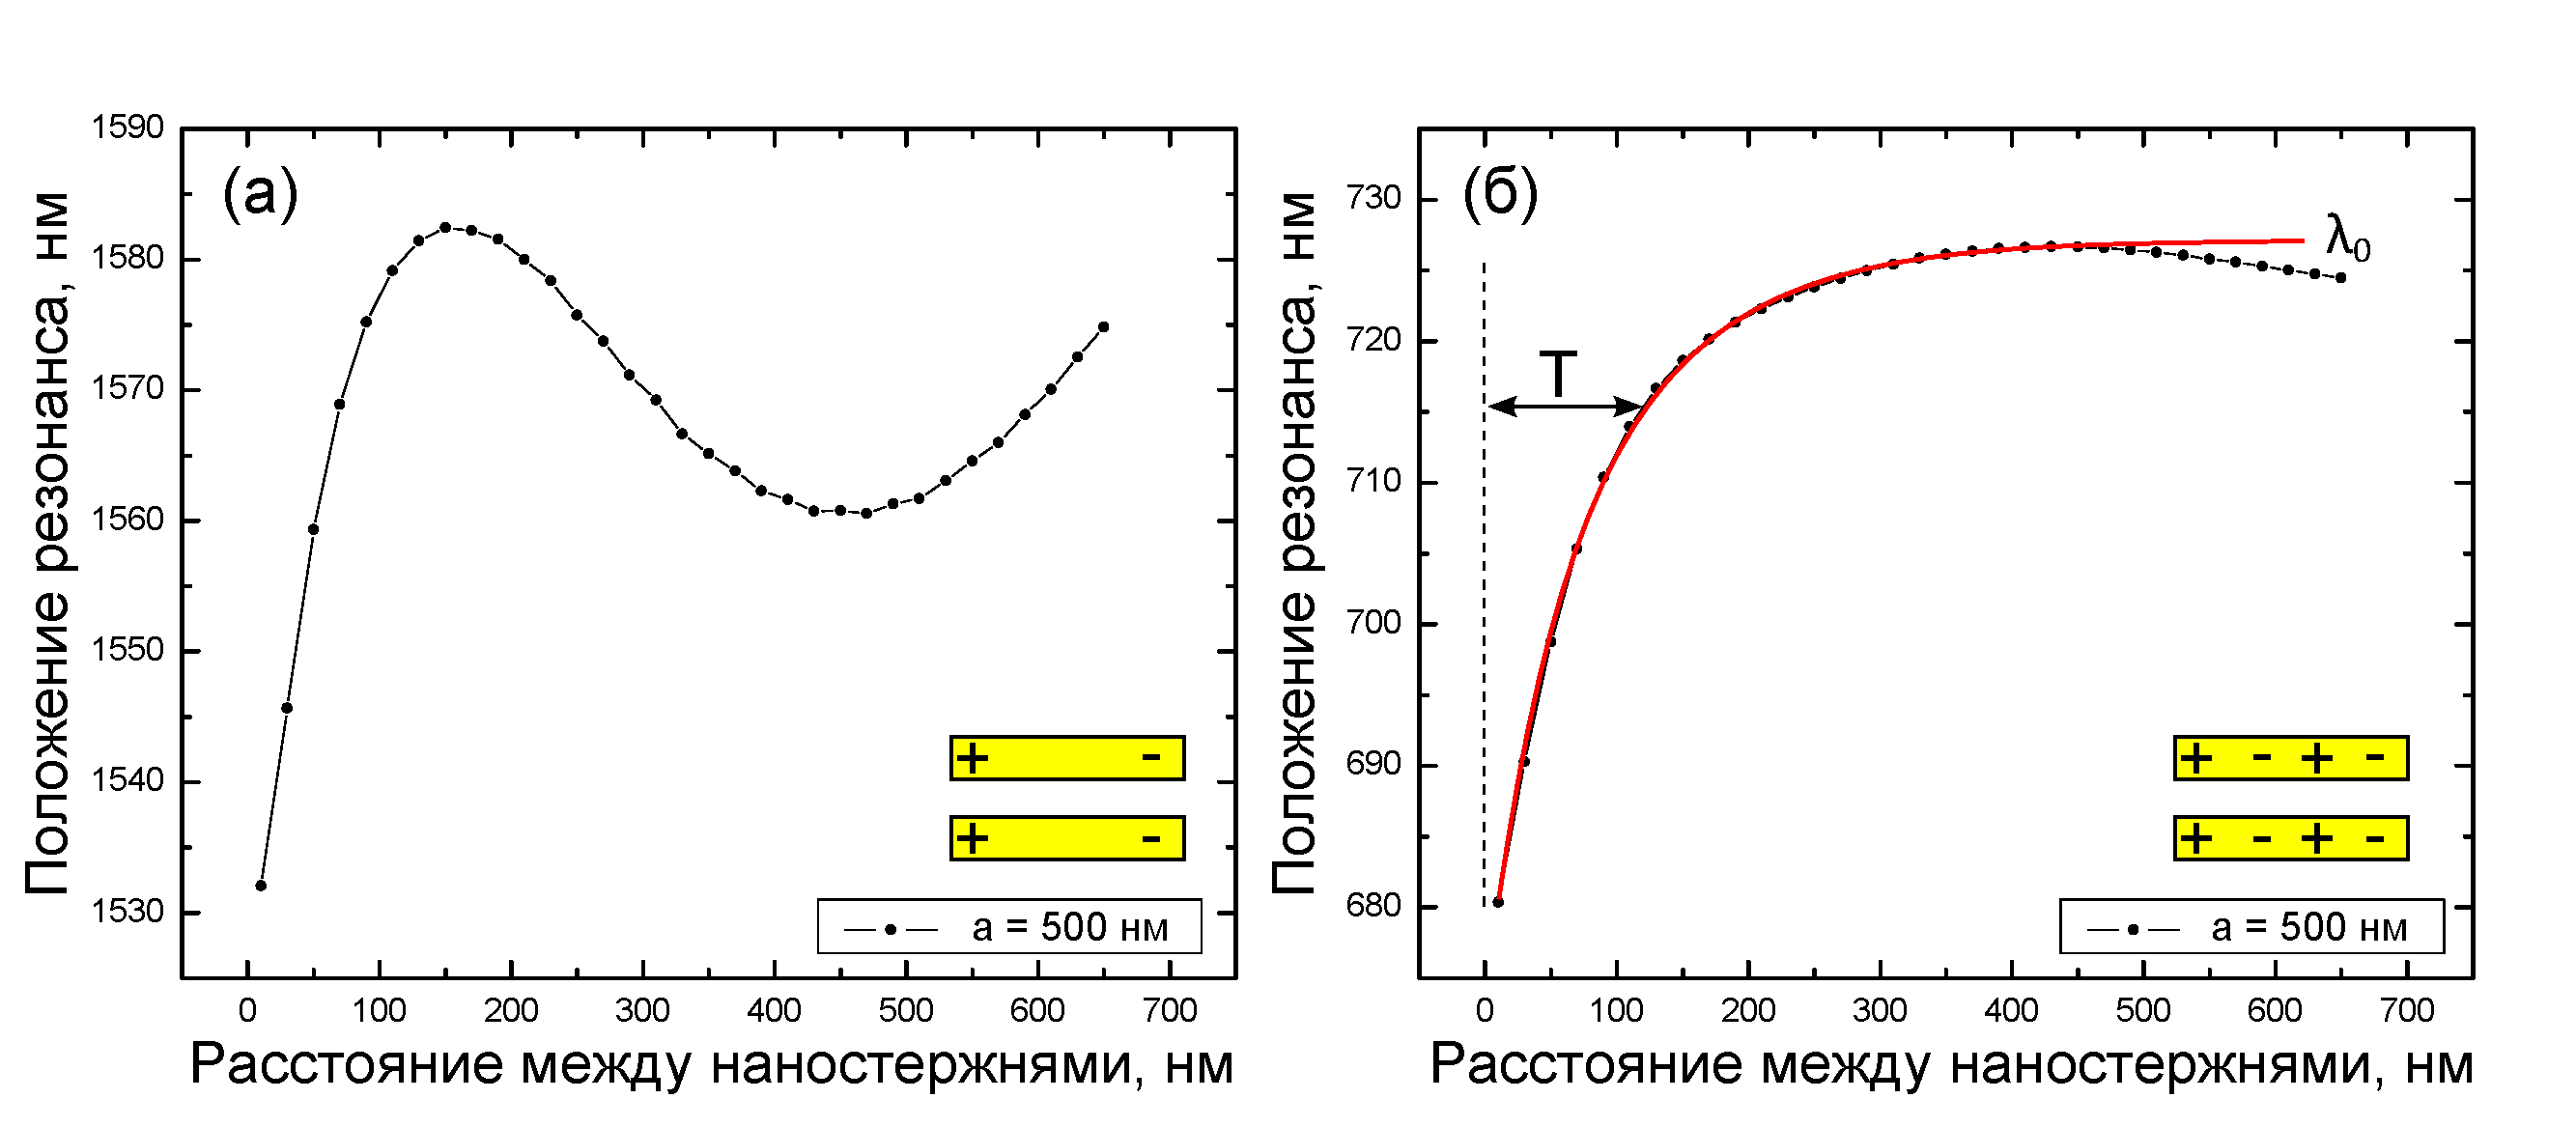
\includegraphics[width=16cm]{img/FDTD/a500PML.pdf}}
\caption{Графики зависимости положения  резонансов первого (а) и второго (б) порядков от расстояния между наностержнями длиной 500 нм. Вставки -- мгновенное распределение зарядов для резонанса первого (а) и второго (б) порядков.}
\label{img:a500PML}
\end{figure}

При уменьшении длины и фиксированном расстоянии наностержней резонансная длина волны смещалась в синюю область. На рис.~\ref{img:a300PML} показана зависимость положения резонасов от расстояния между наностержнями при их длине 300 нм. Видно, что характерные для резонансов первого и второго порядков осцилляции сохраняются, а также сохраняется значение верхней границы применимости <<плазмонной линейки>>, которая определяется равенством нуля первой производной положения резонанса от расстояния между наностержнями и составляет  $ \approx 150 \pm 10 $ нм для резонса первого порядка и $ \approx 400 \pm 30 $ нм для резонанса второго порядка.

\begin{figure}
\center{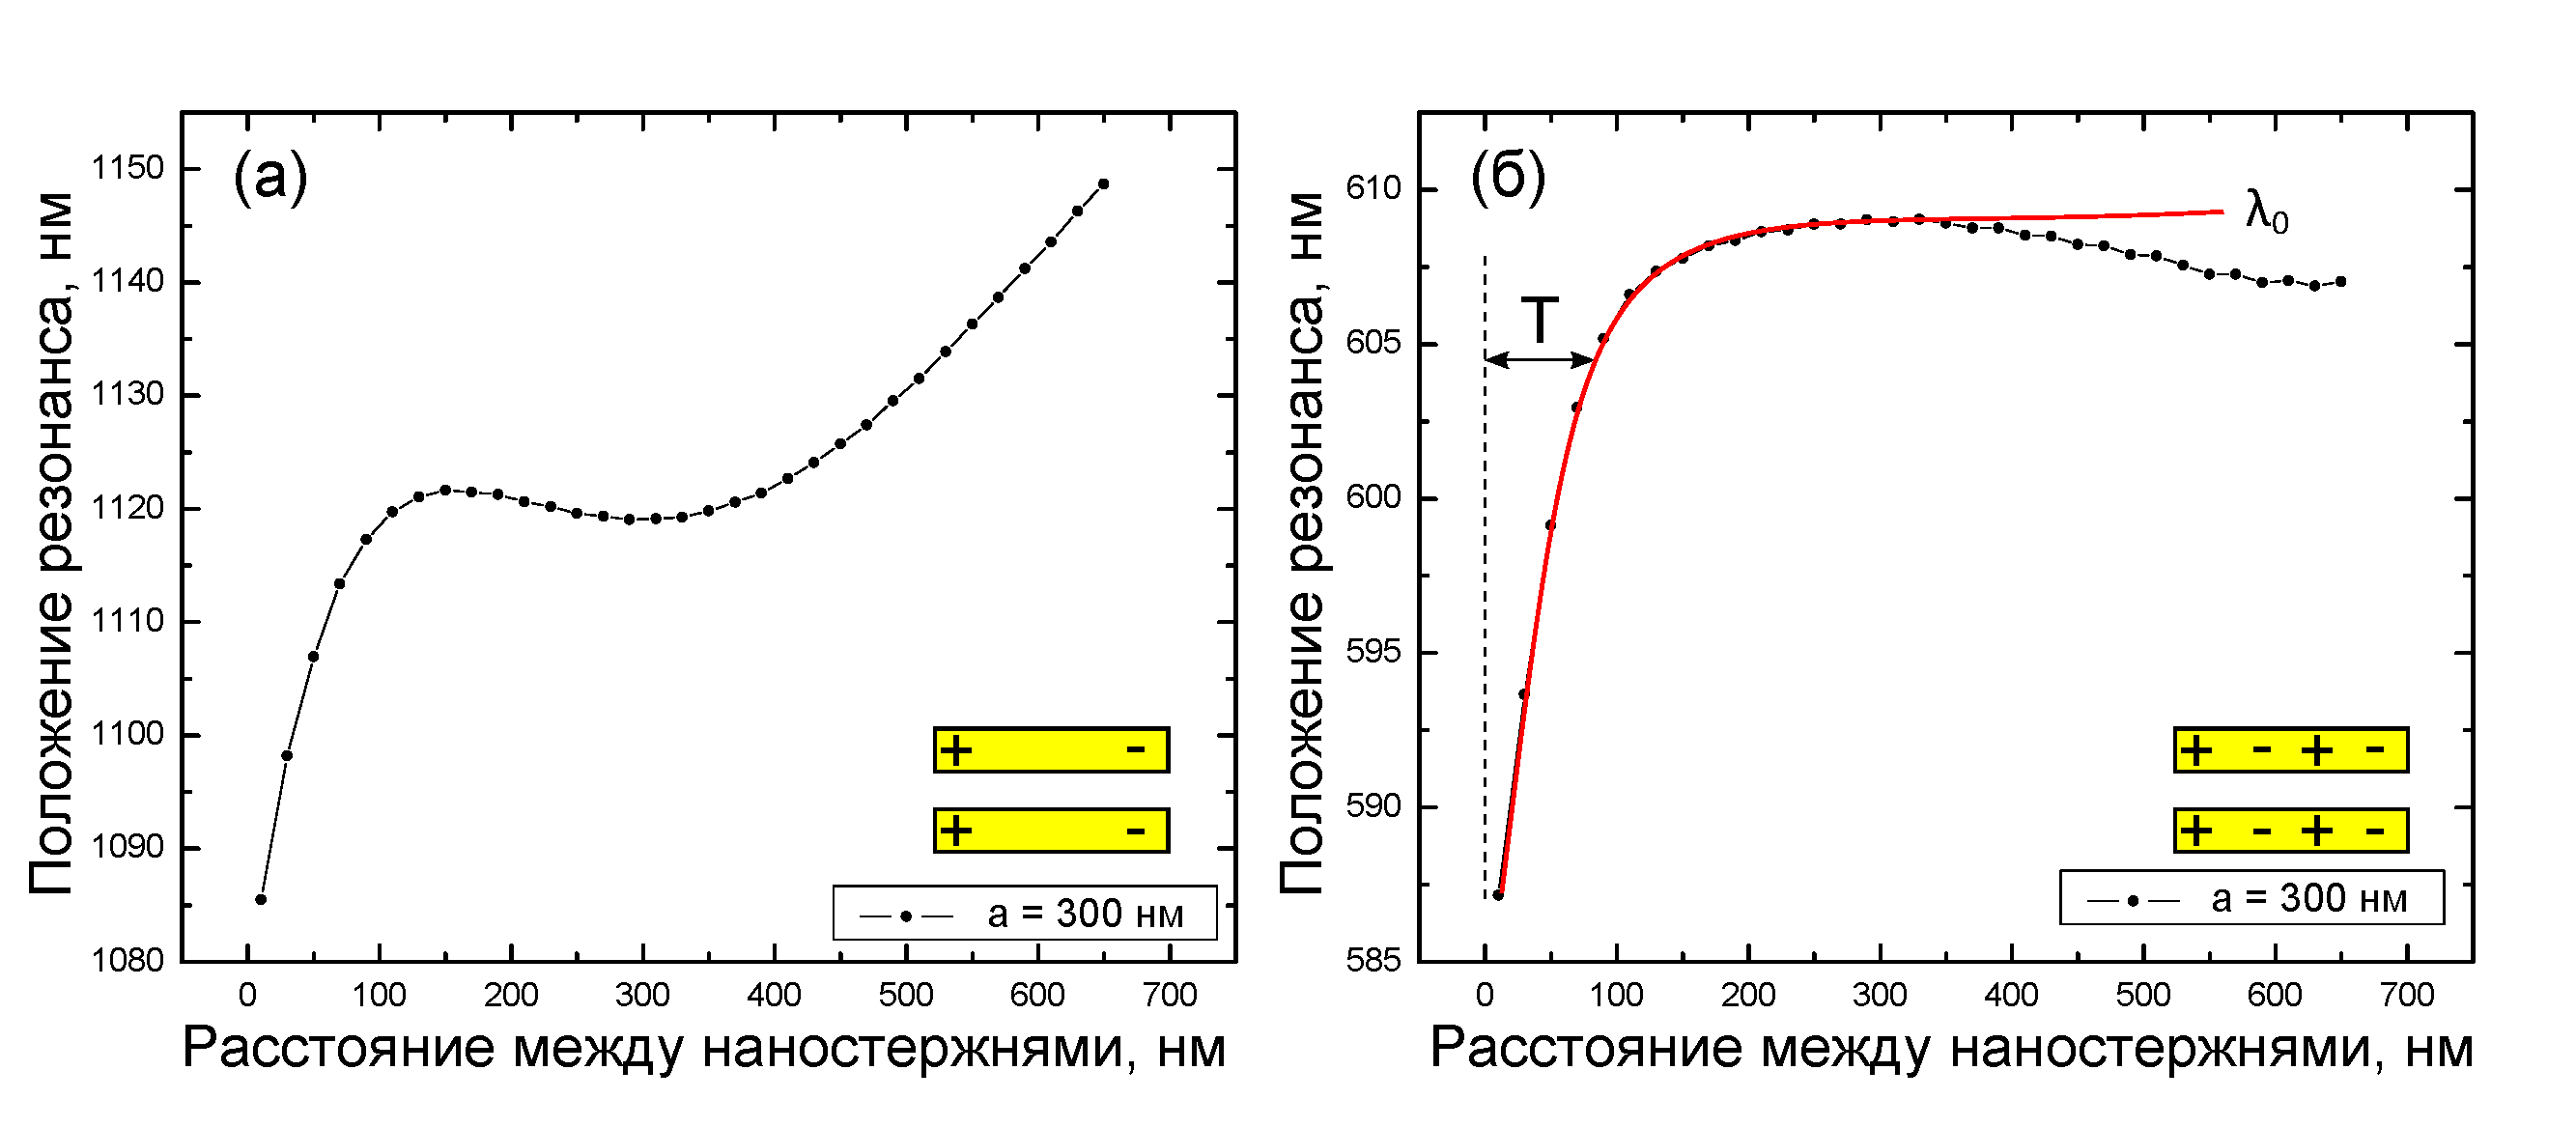
\includegraphics[width=16cm]{img/FDTD/a300PML.pdf}}
\caption{Графики зависимости положения  резонансов первого (a) и второго (б) порядков от расстояния между наностержнями длиной 300 нм. Вставки -- мгновенное распределение зарядов для резонанса первого (a) и второго (б) порядков.}
\label{img:a300PML}
\end{figure}

Далее рассчитывался спектр пропускания для пар наностержней длиной от 100 нм до 500 нм с шагом 50 нм, и для каждой фиксированной длины наностержней рассчитывалась зависимость положения резонанса первого и второго порядков от расстояния между наностержнями. При этом резонанс второго порядка становится различным при длине наностержней 250 нм и больше. Данная зависимость положения резонансов от расстояния между наностержнями аппроксимировалась экспонентой вида $ y(x) = A \exp (-x/ T ) + y_0 $ . График зависимости постоянной затухания $ T $ от длины наностержней показан на рис.~\ref{img:expdecay}а для резонанса первого порядка и на рис.~\ref{img:expdecay}б для резонанса второго порядка.

\begin{figure}
\center{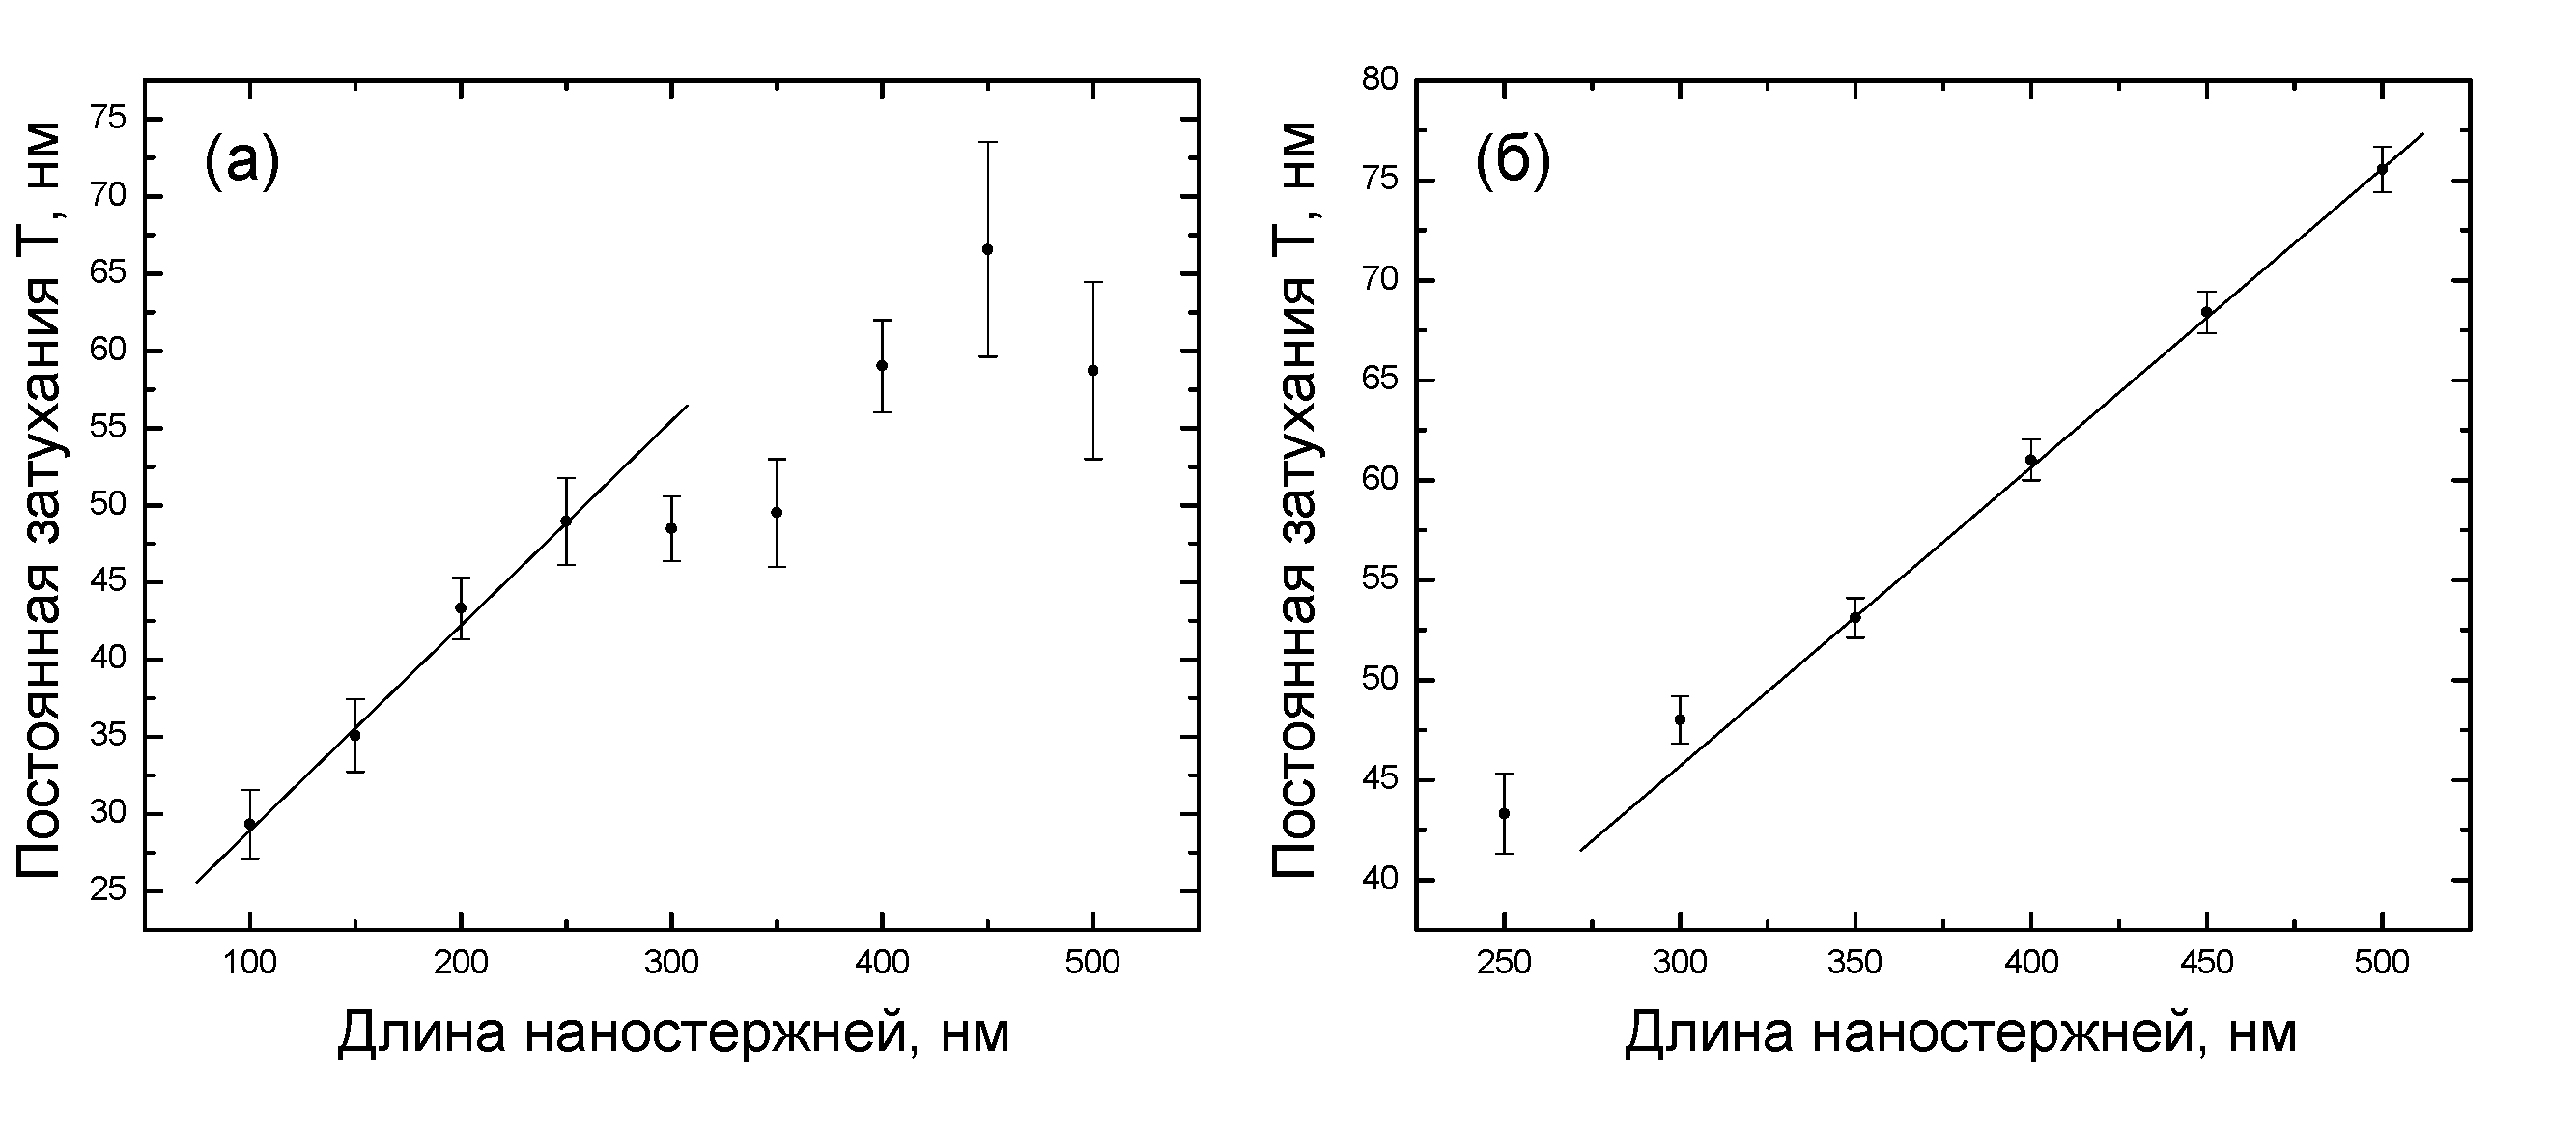
\includegraphics[width=16cm]{img/FDTD/expdecay.pdf}}
\caption{Графики зависимости значения постоянной затухания $ T $ от длины наностержней для резонанса первого порядка (а) и для резонанса второго порядка (б).}
\label{img:expdecay}
\end{figure}

Из графиков видно, что линейная зависимость сохраняется для резонансов первого порядка при длине наностержней от 100 нм до 250 нм, а для резонанса второго порядка при длине наностержней от 350 нм до 500 нм. Значит, для уравнения <<плазмонной линейки>> положение резонанса первого порядка можно использовать для длин наностержней от 100 нм до 250 нм  , а положение резонанса второго порядка --- для длин наностержней от 350 нм до 500 нм.

Пусть $ \lambda_0 $ -- резонансная длина волны, которая определяется соотношением
\begin{equation}
\dfrac{\partial \lambda}{\partial d} \Big|_{\lambda _0} = 0,
\end{equation}
где $ \lambda $ -- длина волны резонанса первого или второго порядков, $ d $ -- расстояние между наностержнями. Тогда график сдвига резонанса первого порядка $ \Delta \lambda =  \lambda - \lambda_0 $ от расстояния между наностержнями для различных длин наностержней показан на рис.~\ref{img:ruler1}а. Далее расстояние нормировалось на геометрический параметр наностержней с размерностью длины, и если расстояние нормировать на квадратный корень из площади $ S $ наностержня, то получается уравнение для <<плазмонной линейки>>:
\begin{equation}
\frac{\Delta \lambda}{\lambda_0} \approx 0.044 \exp \left( - 2.38 \frac{d}{\sqrt{S}} \right).
\label{eq:ruler1}
\end{equation}
График кривой, описывающейся уравнением (\ref{eq:ruler1}), показан на рис.~\ref{img:ruler1}б сплошной черной линией, а точками показаны положения относительного сдвига резонансов первого порядка для наностержней с длиной 100, 150, 200 и 250 нм.

\begin{figure}
\center{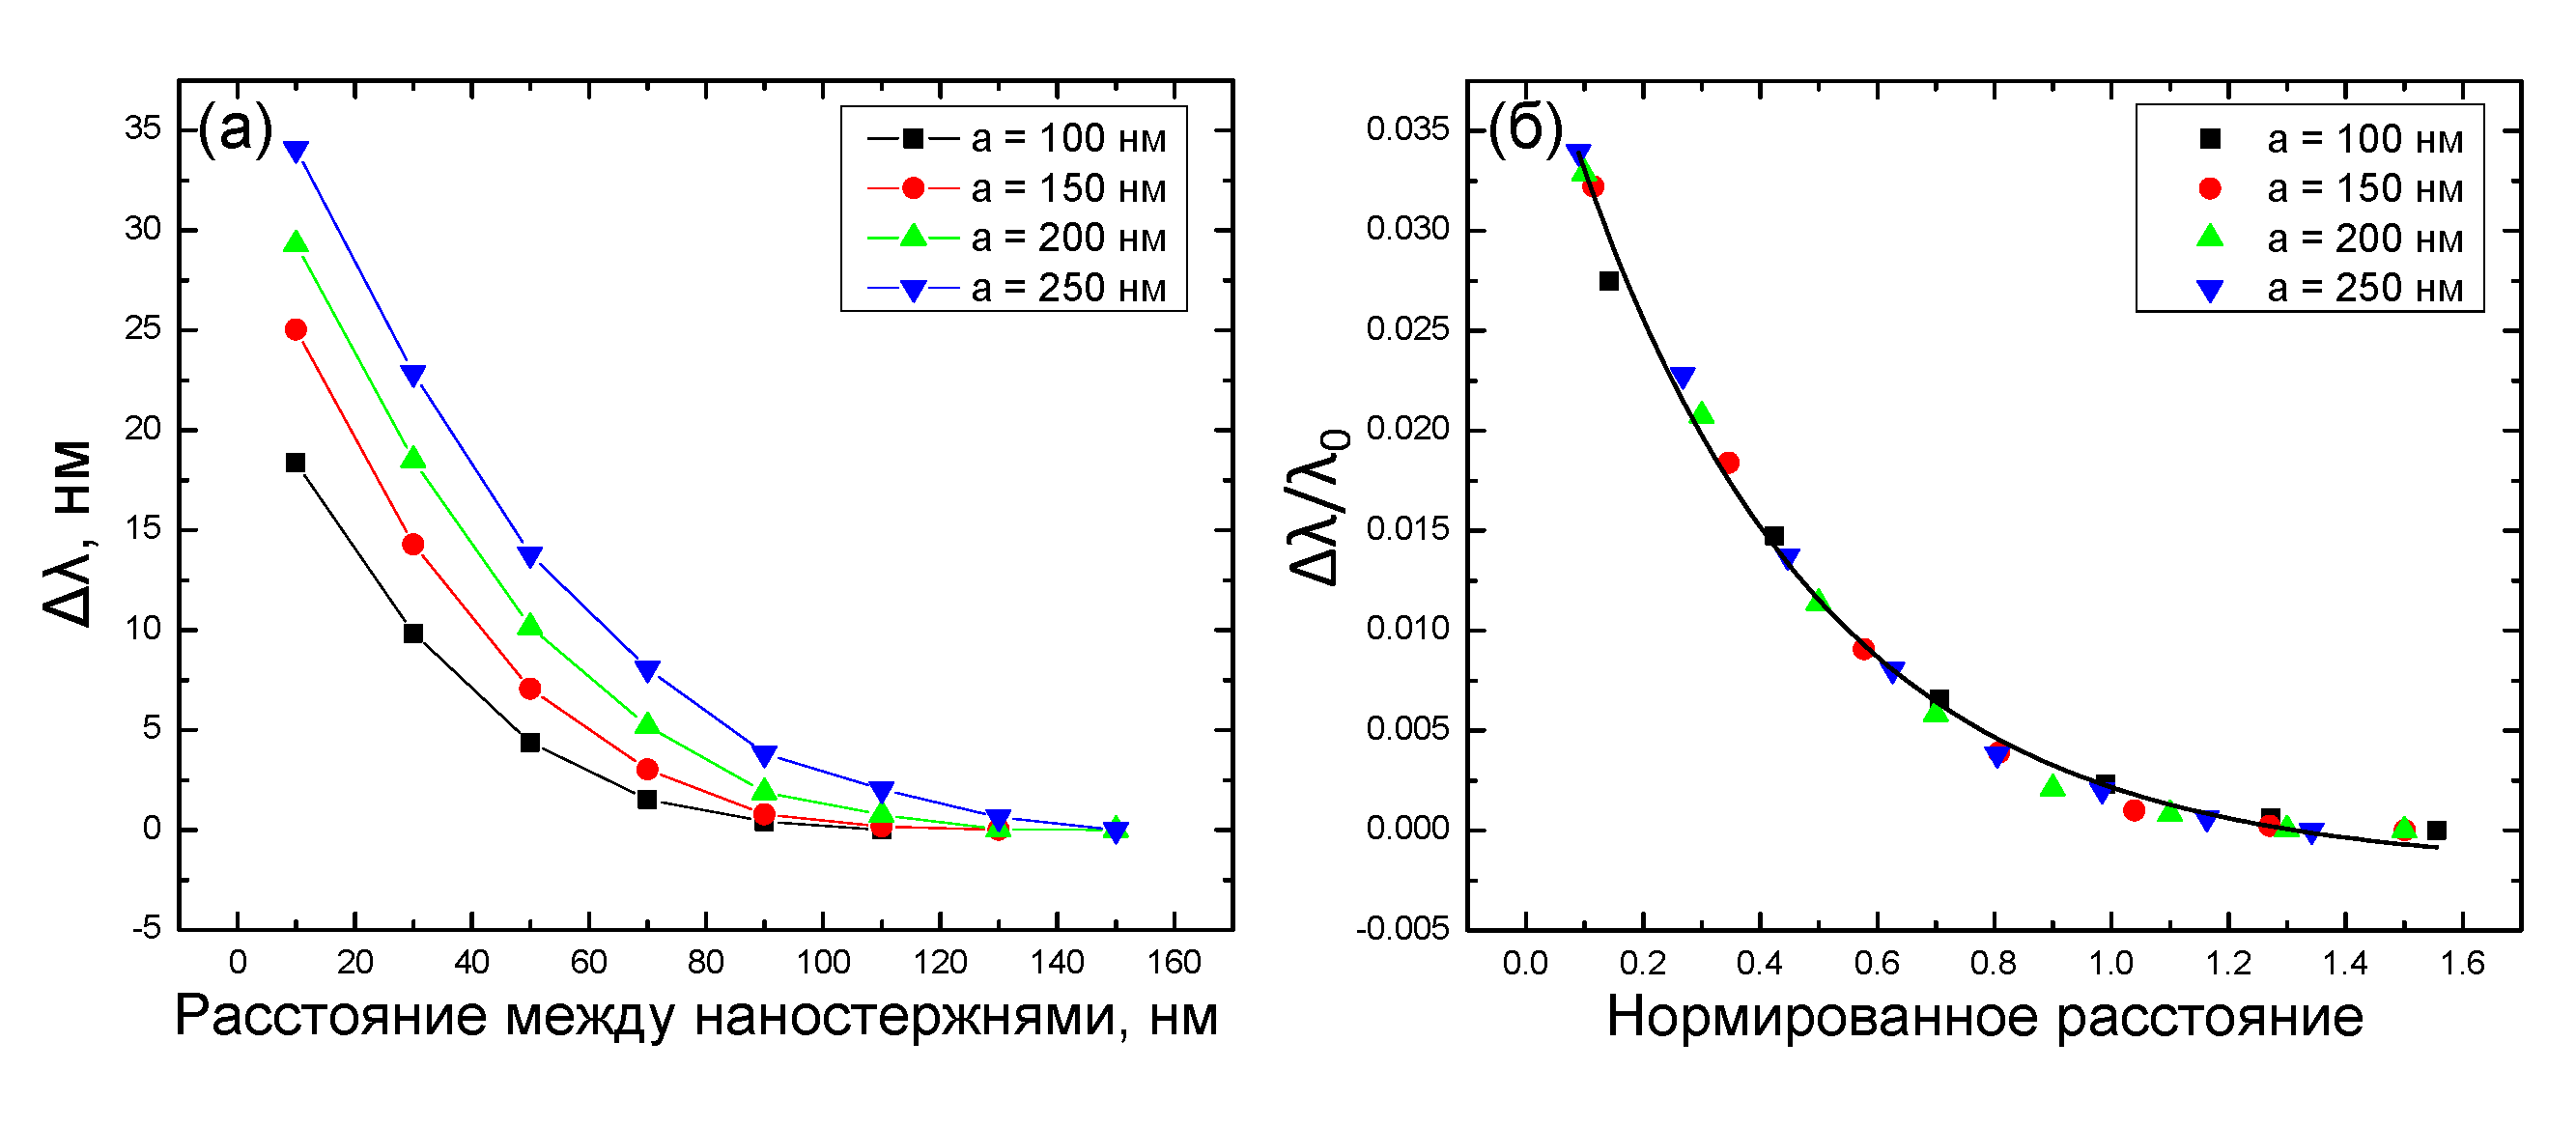
\includegraphics[width=16cm]{img/FDTD/ruler_res1.pdf}}
\caption{Графики зависимости сдвига резонанса первого порядка $ \Delta \lambda $ от расстояния между наностержнями (а) и зависимость относительного сдвига резонанса первого порядка от нормированного на квадратный корень из площади наностержня расстояния (б) при длине наностержней 100, 150, 200 и 250 нм. }
\label{img:ruler1}
\end{figure}

Для резонанса второго порядка также можно получить уравнение <<плазмонной линейки>>, если расстояние между наностержнями нормировать на длину наностержней $ a $. Тогда уравнение выглядит следующим образом:
\begin{equation}
\frac{\Delta \lambda}{\lambda_0} \approx 0.063 \exp \left( - 6.62 \frac{d}{a} \right).
\end{equation}
Графики зависимости сдвига резонанса второго порядка $ \Delta \lambda $ от расстояния между наностержнями и зависимость относительного сдвига резонанса второго порядка от нормированного расстояния при длине наностержней 350, 400, 450 и 500 нм показаны на рис.~\ref{img:ruler2}.

\begin{figure}
\center{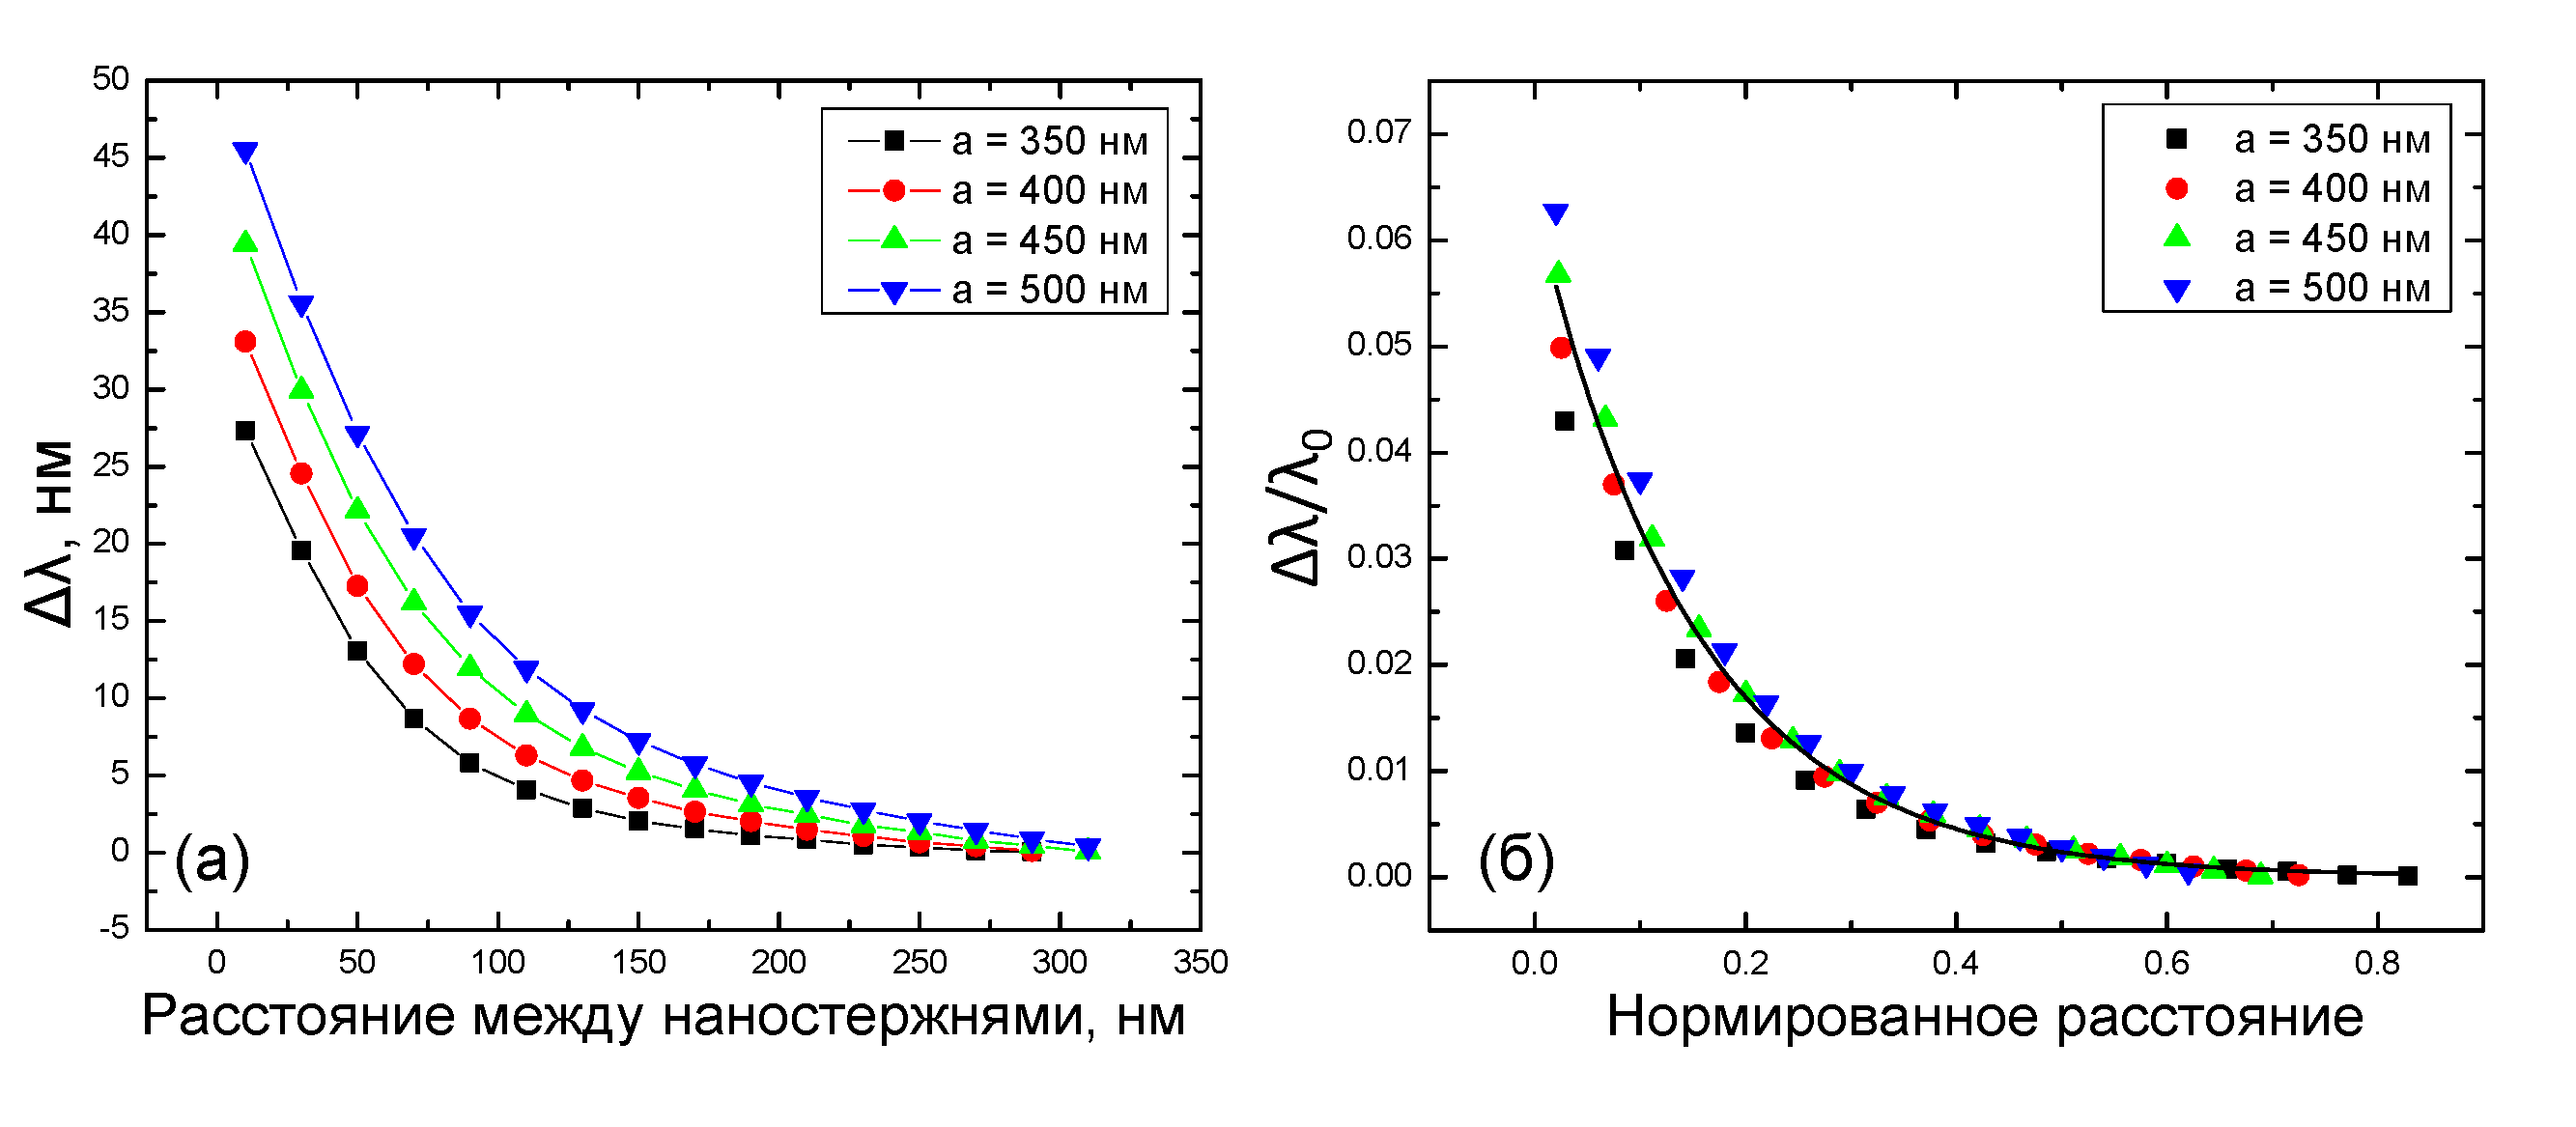
\includegraphics[width=16cm]{img/FDTD/ruler_res2.pdf}}
\caption{Графики зависимости сдвига резонанса второго порядка $ \Delta \lambda $ от расстояния между наностержнями (а) и зависимость относительного сдвига резонанса второго порядка от нормированного на длину  наностержня расстояния (б) при длине наностержней 350, 400, 450 и 500 нм }
\label{img:ruler2}
\end{figure}

Как правило, в экспериментальных исследованиях измеряется спектр не одиночной пары наночастиц, а ансамбля из пар наночастиц с фиксированным расстоянием между ними, как показано на рис.~\ref{img:PR_SEM}. Поэтому вместо граничных условий PML в плоскостях XZ и YZ были выбраны периодические граничные условия. Тогда размер интегрирования вдоль осей $ Ox $ и $ Oy $ можно интерпретировать как период между ансамблями спаренных наностержней. На рис.~\ref{img:BCperiod} показана зависимость коэффициента пропускания от длины волны и периода между ансамблями из спаренных наностержней. Видно, что положение резонанса также зависит и от периода между ансамблями из спаренных наностержней, что говорит о наличии дальнепольного дифракционного взаимодействия  вплоть до периода в 3 мкм. Для длины волны $ \lambda \approx 600$ нм наблюдается резонанс второго порядка, который менее чувствителен к периоду структуры.

\begin{figure}
\center{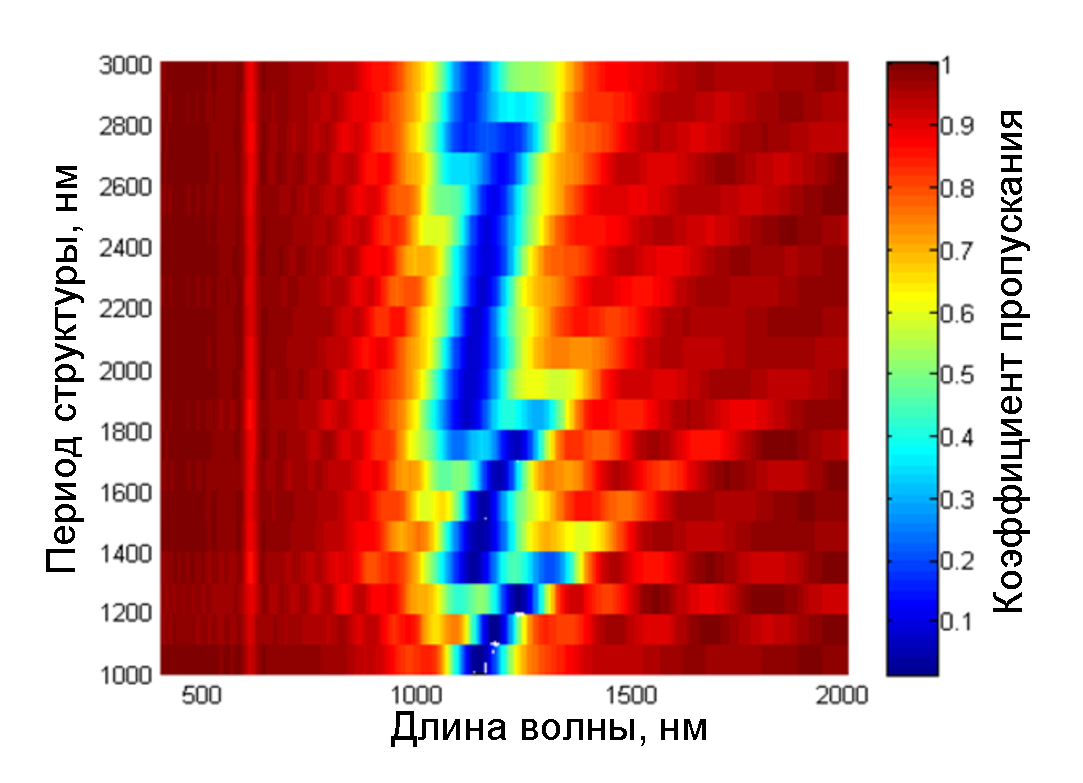
\includegraphics[width=10cm]{img/FDTD/BCperiod.pdf}}
\caption{График зависимости коэффициента пропускания от длины волны падающего электромагнитного излучения и периода между ансамблями из спаренных наностержней. Длина наностержней составляет 300 нм, а расстояние между ними -- 300 нм.}
\label{img:BCperiod}
\end{figure}

Таким образом, в результате численных расчетов  обнаружено наличие двух резонансов ЛПП  с различным локальным распределением плотности мощности для наностержней длиной до 500 нм, исследовано локальное распределение плотности мощности электромагнитного поля вблизи наностержней при резонансах различных порядков, а также на основе смещения положения резонансов первого и второго порядков были получены уравнения для <<плазмонных линеек>>.


\section{Экспериментальные данные}

Резонанс ЛПП димеров исследовался с помощью микроспектроскопии пропускания. Схема экспериментальной установки показана на рис.~\ref{img:expsetup}.
\begin{figure}
\center{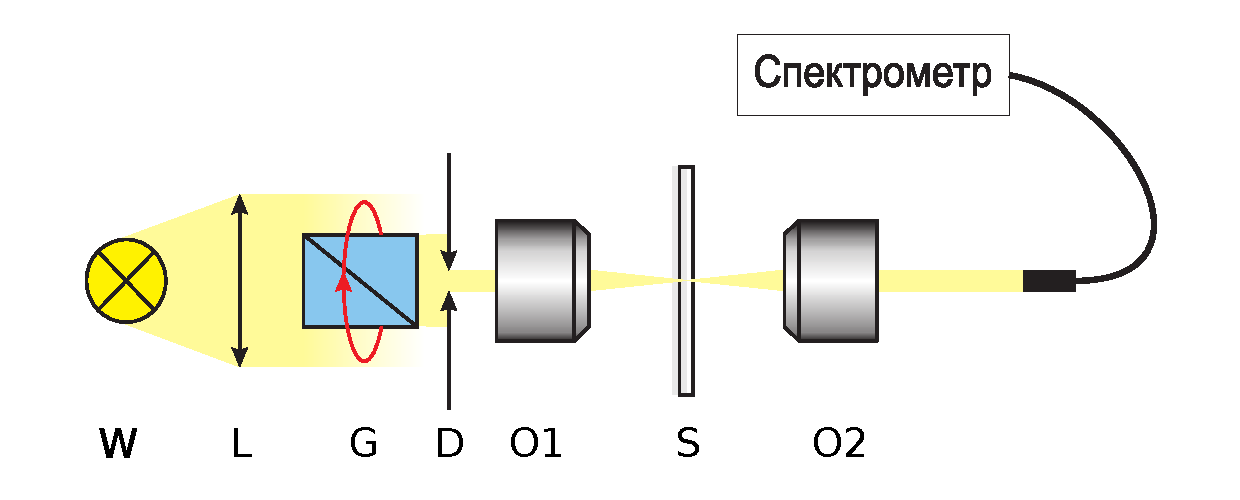
\includegraphics[width=12cm]{img/microspectroscopy/exp_setup.pdf}}
\caption{Схема экспериментальной установки. W --- источник света, L --- собирающая линза для формирования параллельного пучка света, G --- призма Глана-Тейлора для преобразования излучения в линейно поляризованное, O1, O2 --- система из двух объективов, S --- исследуемый образец. }
\label{img:expsetup}
\end{figure}
Спектры пропускания получались следующим образом: снимался спектр пропускания образца $ S_{sig} $, потом на расстоянии $ \approx 100 $ мкм от ансамбля димеров снимался спектр пропускания подложки $ S_{back} $. Конечный спектр пропускания $ S $ образцов определялся следующим образом:
\begin{equation}
S = \frac{S_{sig}}{S_{back}}.
\end{equation}
Для избавления от шумов каждая точка спектра сглаживалась по 15ти соседним с гауссовым весом. При определении положения резонанса выбиралась точка с минимальным коэффициентом пропускания, а также 10 соседних точек, и полученная кривая аппроксимировалась параболой $ y(x) = y_0 + (x - x_0)^2 $, где точка $ x_0 $ являлась положением резонанса ЛПП. Обработка данных производилась с помощью скрипта, написанного на языке программирования PYTHON. 

При получении спектров пропускания было выбрано два направления поляризации: параллельное наностержням и перпендикулярное им. При падении света с поляризацией, перпендикулярной наностержням, наблюдался небольшой сдвиг резонанса ЛПП в красную область спектра при уменьшении расстояния между наностержнями. И наоборот, при падении света с поляризацией, параллельной наностержням, наблюдался сдвиг в синюю область спектра при уменьшении расстояния между наностержнями. На рис.~\ref{img:Spectraa5d3} показан типичный спектр пропускания для света с поляризацией, параллельной наностержням. При этом наблюдается резонанс второго порядка, так как глубина модуляции составляет 5 \% и резонансная длина волны лежит не в инфракрасной области, как и в численных расчетах.
\begin{figure}
\center{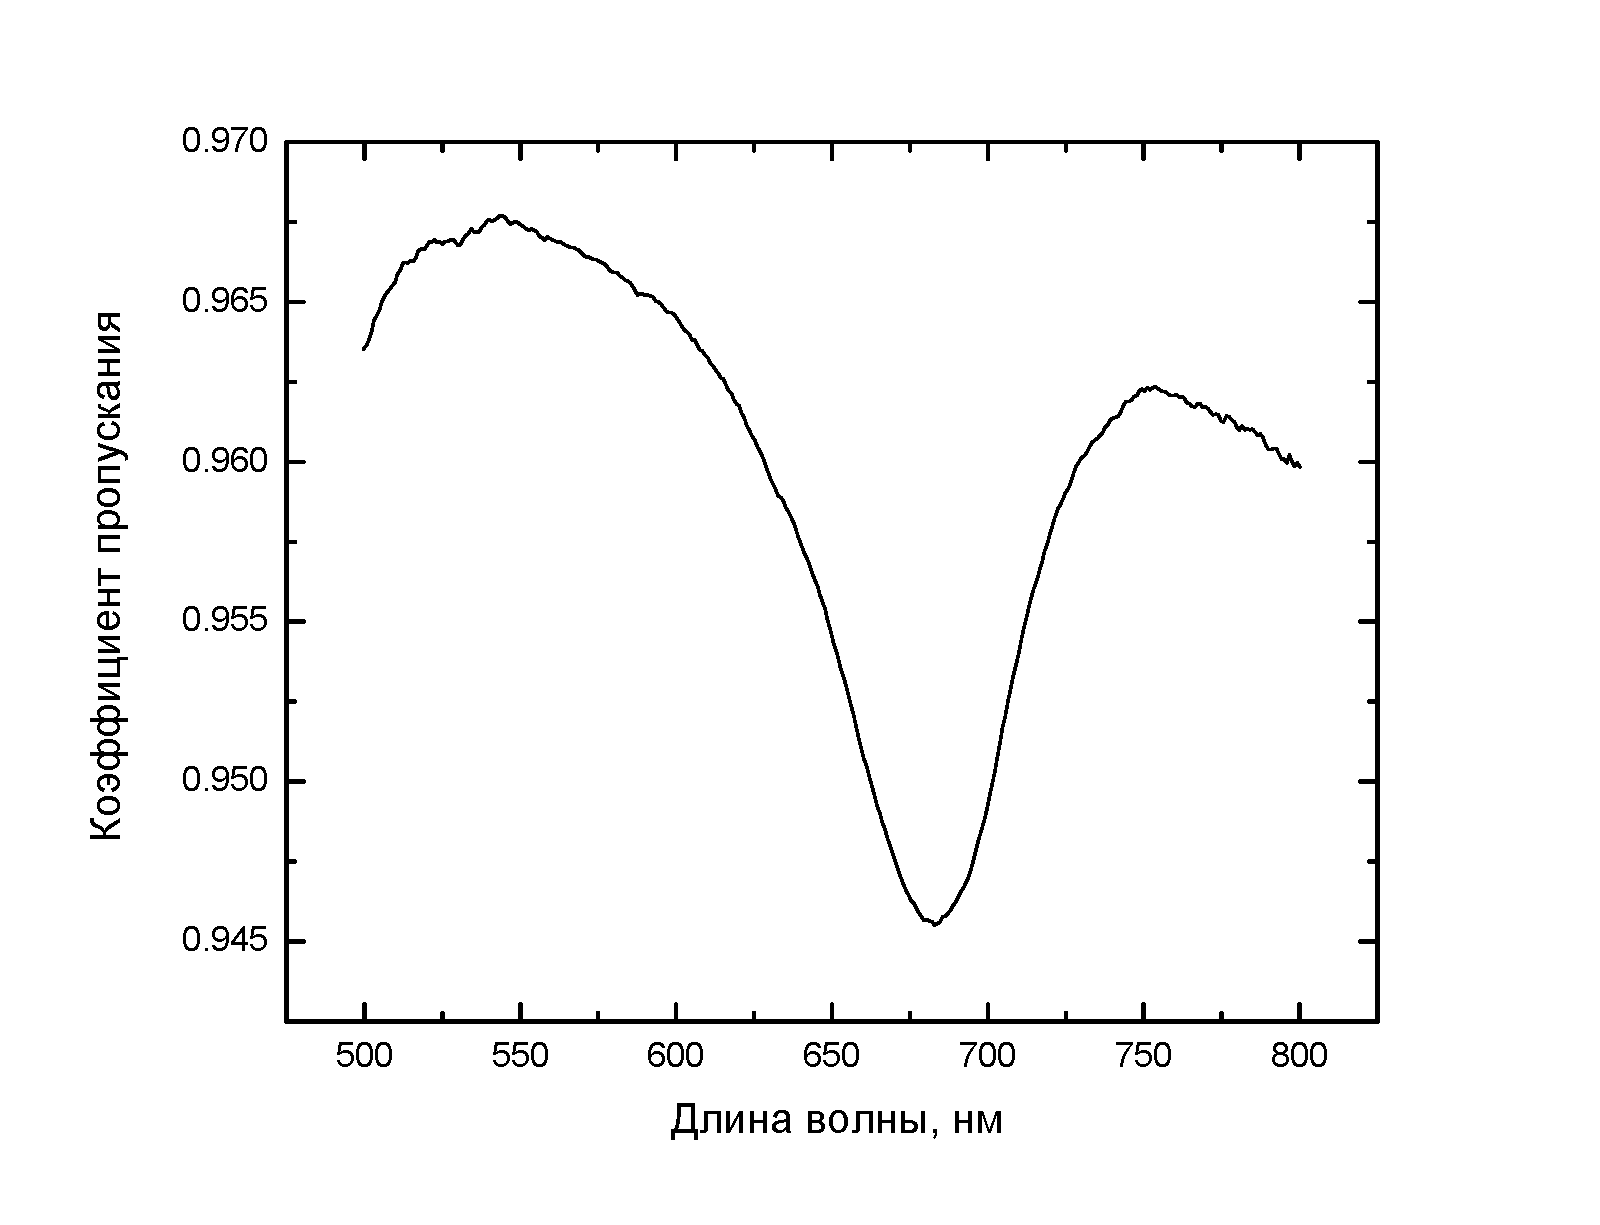
\includegraphics[width=10cm]{img/microspectroscopy/a400d300_spectra.pdf}}
\caption{Спектр пропускания ансамбля из наностержней с длиной 400 нм и расстоянием 250 нм между ними.}
\label{img:Spectraa5d3}
\end{figure}
На рис.~\ref{img:a500simexp} показана зависимость положения резонанса второго порядка как функция расстояния между наностержнями для длин наностержней 500 нм, рассчитанная численно (рис.~\ref{img:a500simexp}a) и полученная экспериментально (рис.~\ref{img:a500simexp}б). На экспериментальном графике нанесены систематические ошибки, которые рассчитывались следующим образом. Для фиксированного расстояния между наностержнями в 110 нм рассчитывалось численно положение резонанса второго порядка для длин наностержней 450 нм и 500 нм. Положение резонанса при этом составляло 685 нм и 713 нм. Так как погрешность в длине при изготовлении образцов составляла 3 нм, то систематическая ошибка определения положения резонанса ЛПП  $ \sigma_{err} \approx 2 $ нм. Видно, что абсолютные значения положения резонанса различаются в численном расчете и в эксперименте примерно на 100 нм. Это связано с тем, что численном расчете не учитывалась кварцевая подложка, которая влияет на положение резонанса ЛПП.
\begin{figure}
\center{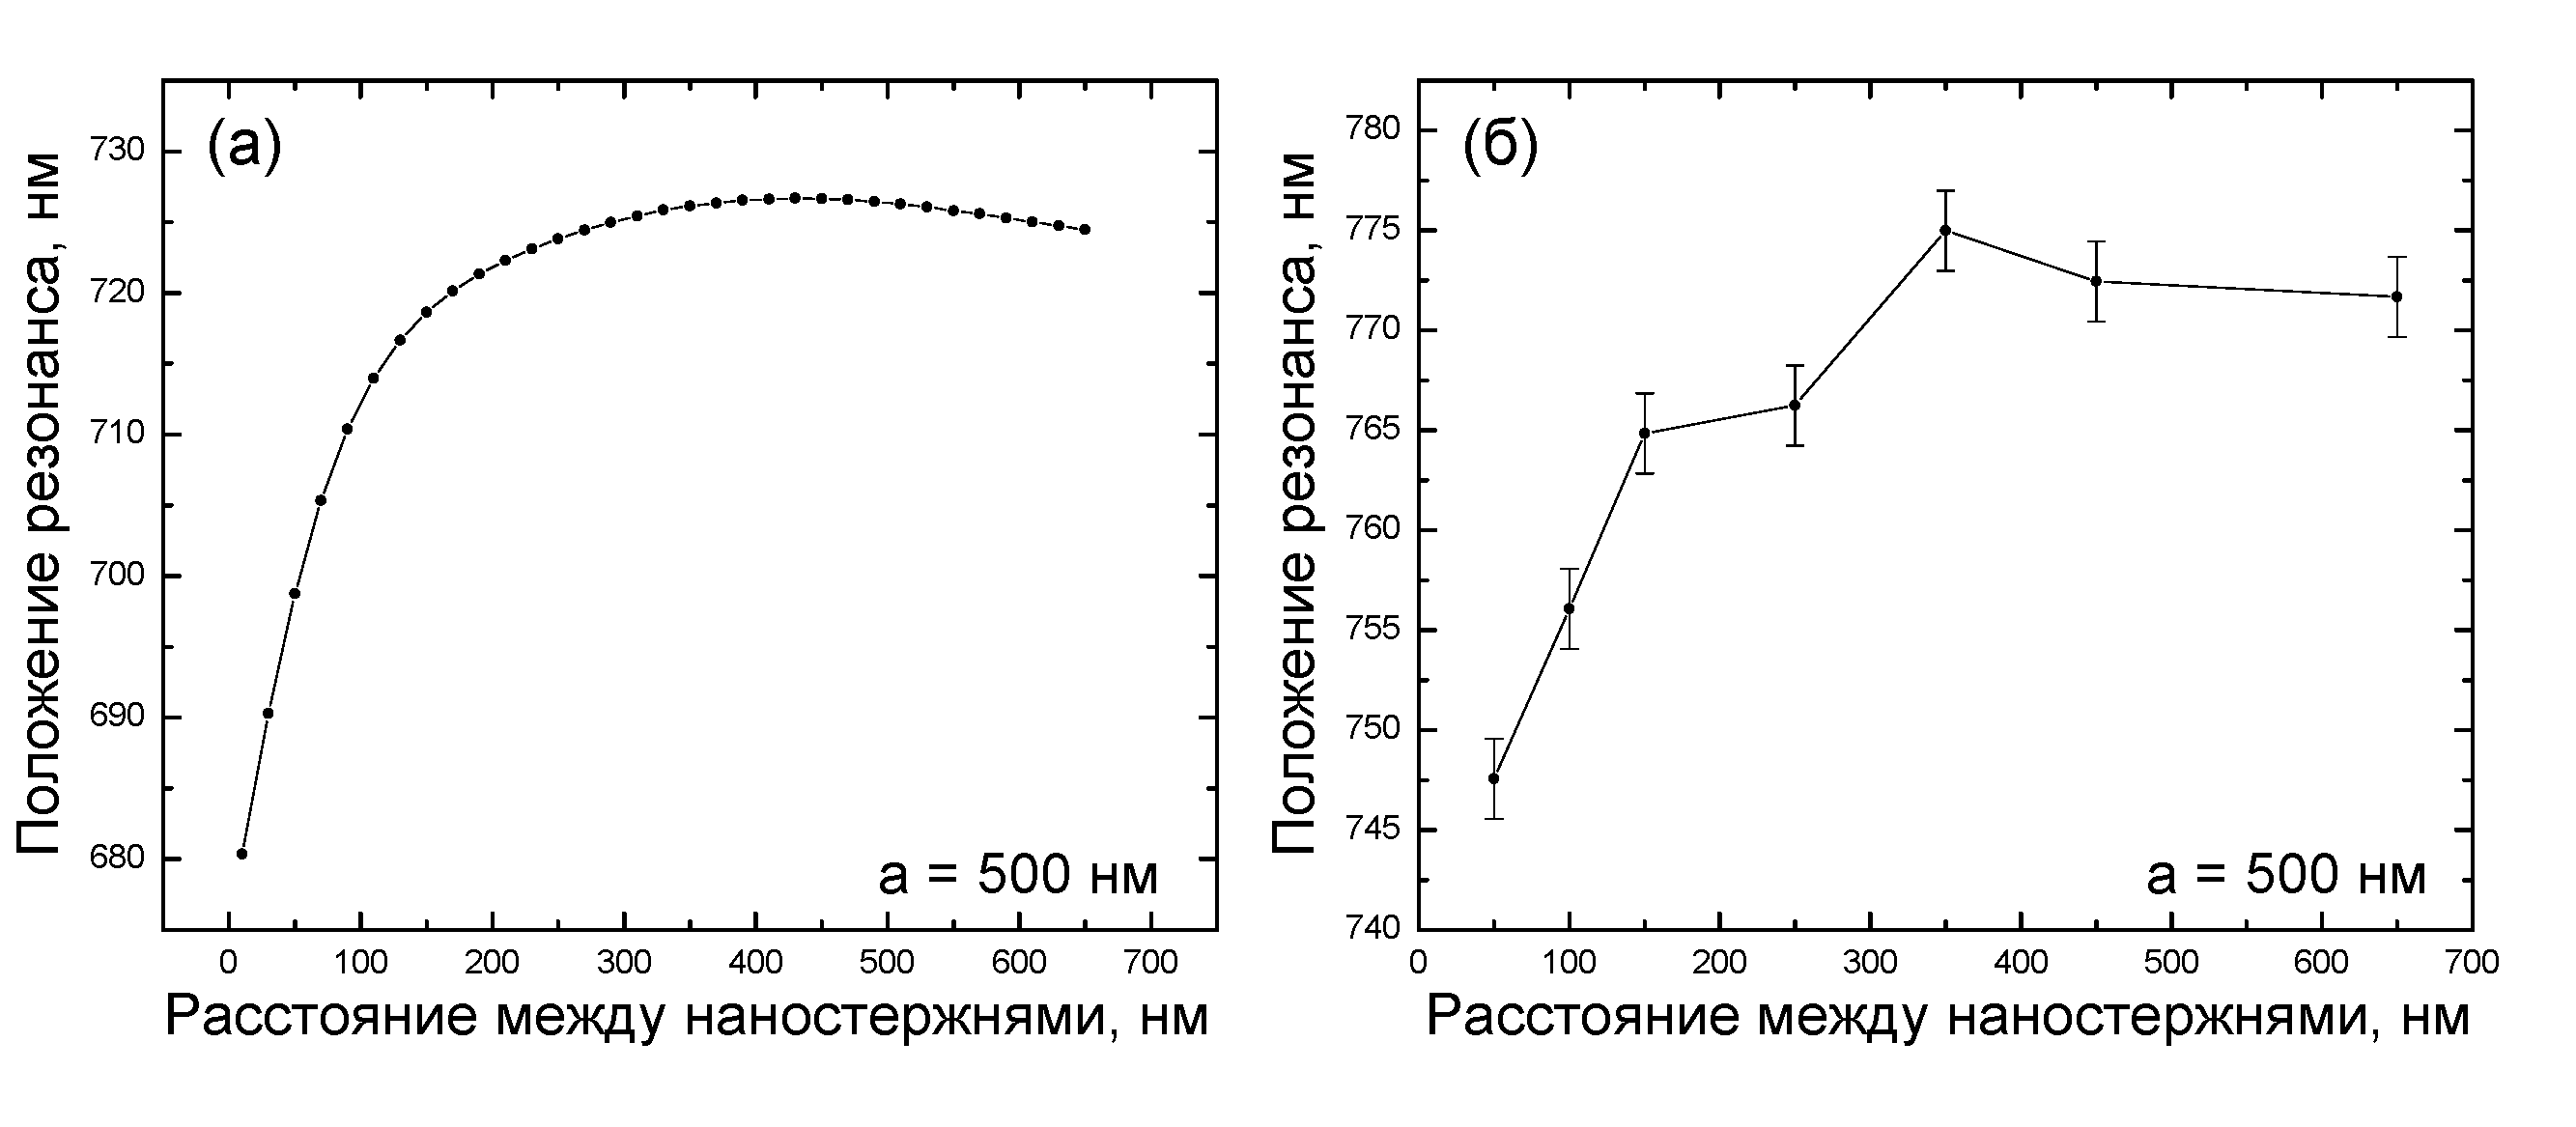
\includegraphics[width=16cm]{img/microspectroscopy/a500simexp.pdf}}
\caption{Рассчитанный численно (а) и полученный экспериментально (б) график зависимости положения резонанса второго порядка от расстояния между наностержнями для длин наностержней 500 нм. }
\label{img:a500simexp}
\end{figure}
\begin{figure}
\center{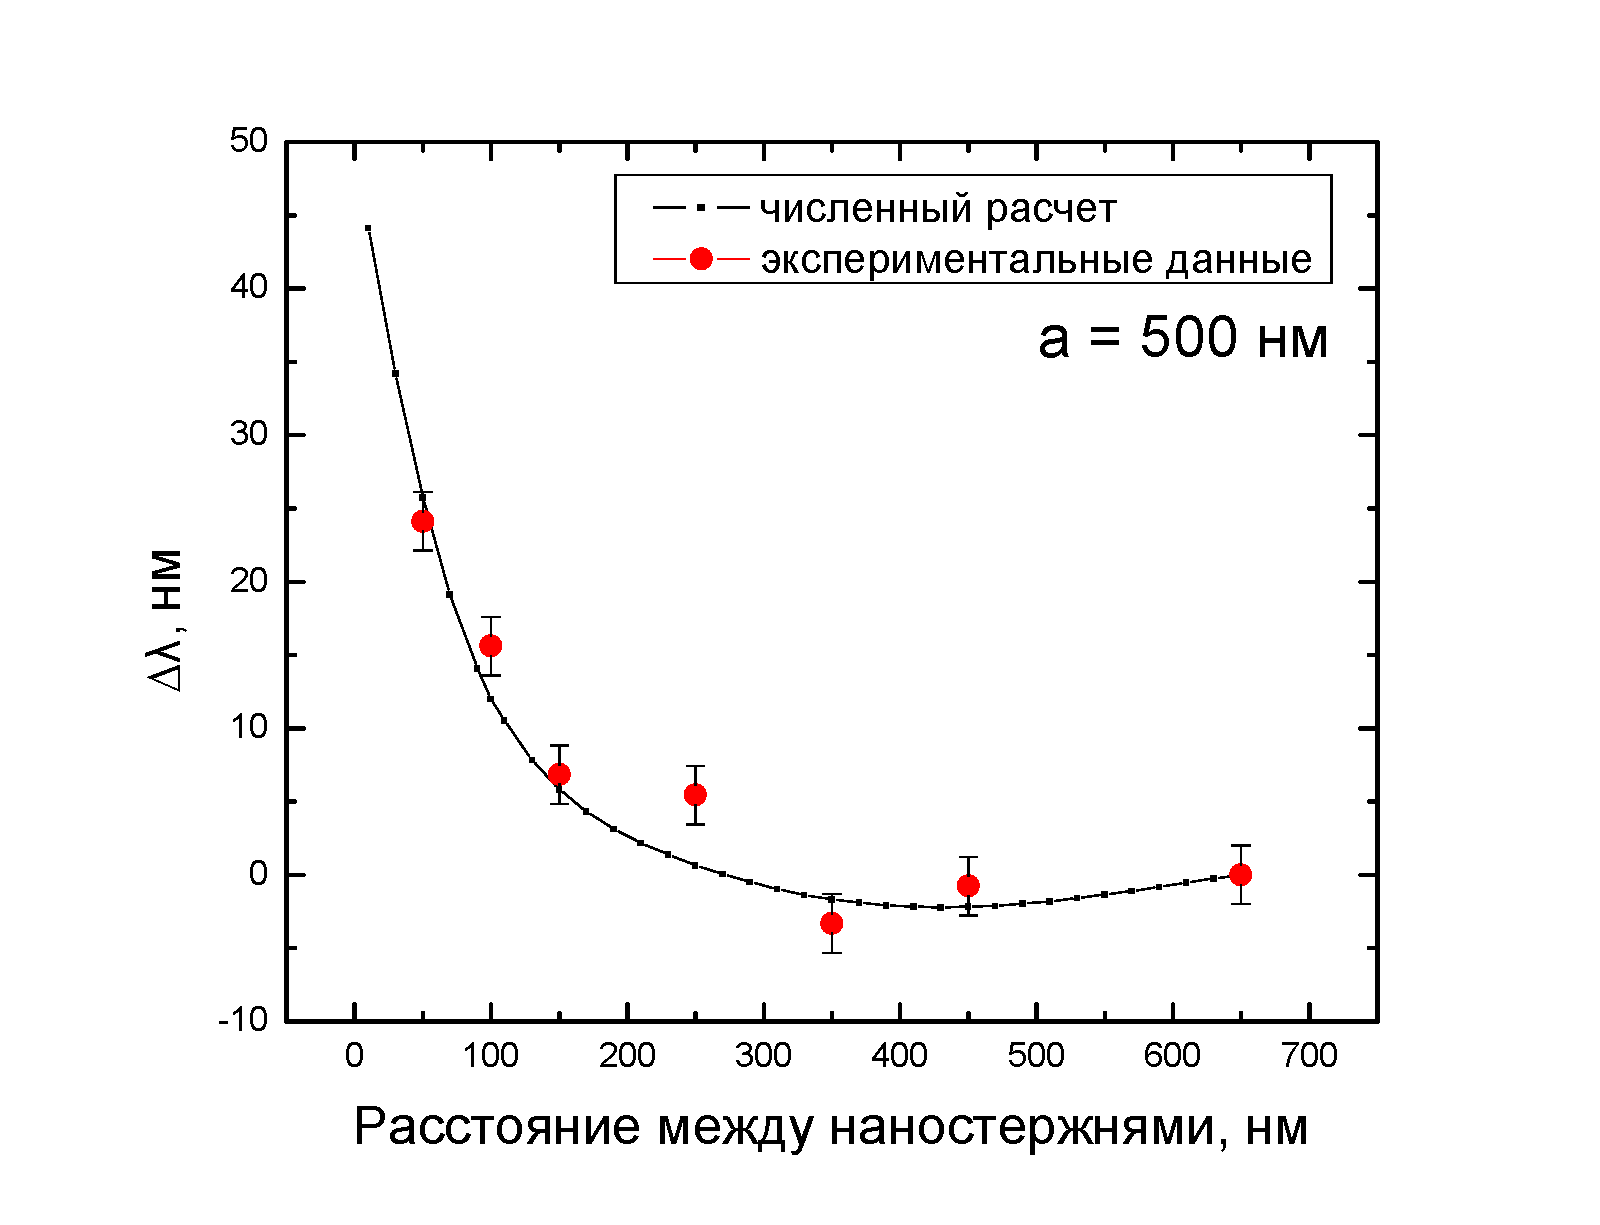
\includegraphics[width=10cm]{img/microspectroscopy/a500shift.pdf}}
\caption{График относительного сдвига резонанса второго порядка от расстояния между наностержнями при длине наностержней 500 нм.}
\label{img:a500shift}
\end{figure}

График относительного сдвига резонанса второго порядка показан на рис.~\ref{img:a500shift}. Здесь линией обозначены данные численного расчета, а красными точками -- экспериментальные данные. Видно, что численный расчет и экспериментальные данные сходятся в пределах погрешности за исключением точки, в которой расстояние между наностержнями составляет 250 нм. Это может быть связано с дальнепольным дифракционным взаимодействием, которое также влияет на положение резонанса.

Для пар наностержней длиной 400 нм также были получены численные и экспериментальные зависимости положения резонанса второго порядка от расстояния между наностержнями и  представлены на рис.~\ref{img:a400simexp}. Видно, что с уменьшением длины нанопалочек резонанс ЛПП сдвигается в синюю область. График относительного сдвига резонанса второго порядка от расстояния между наностержнями показан на рис.~\ref{img:a400shift}.
\begin{figure}
\center{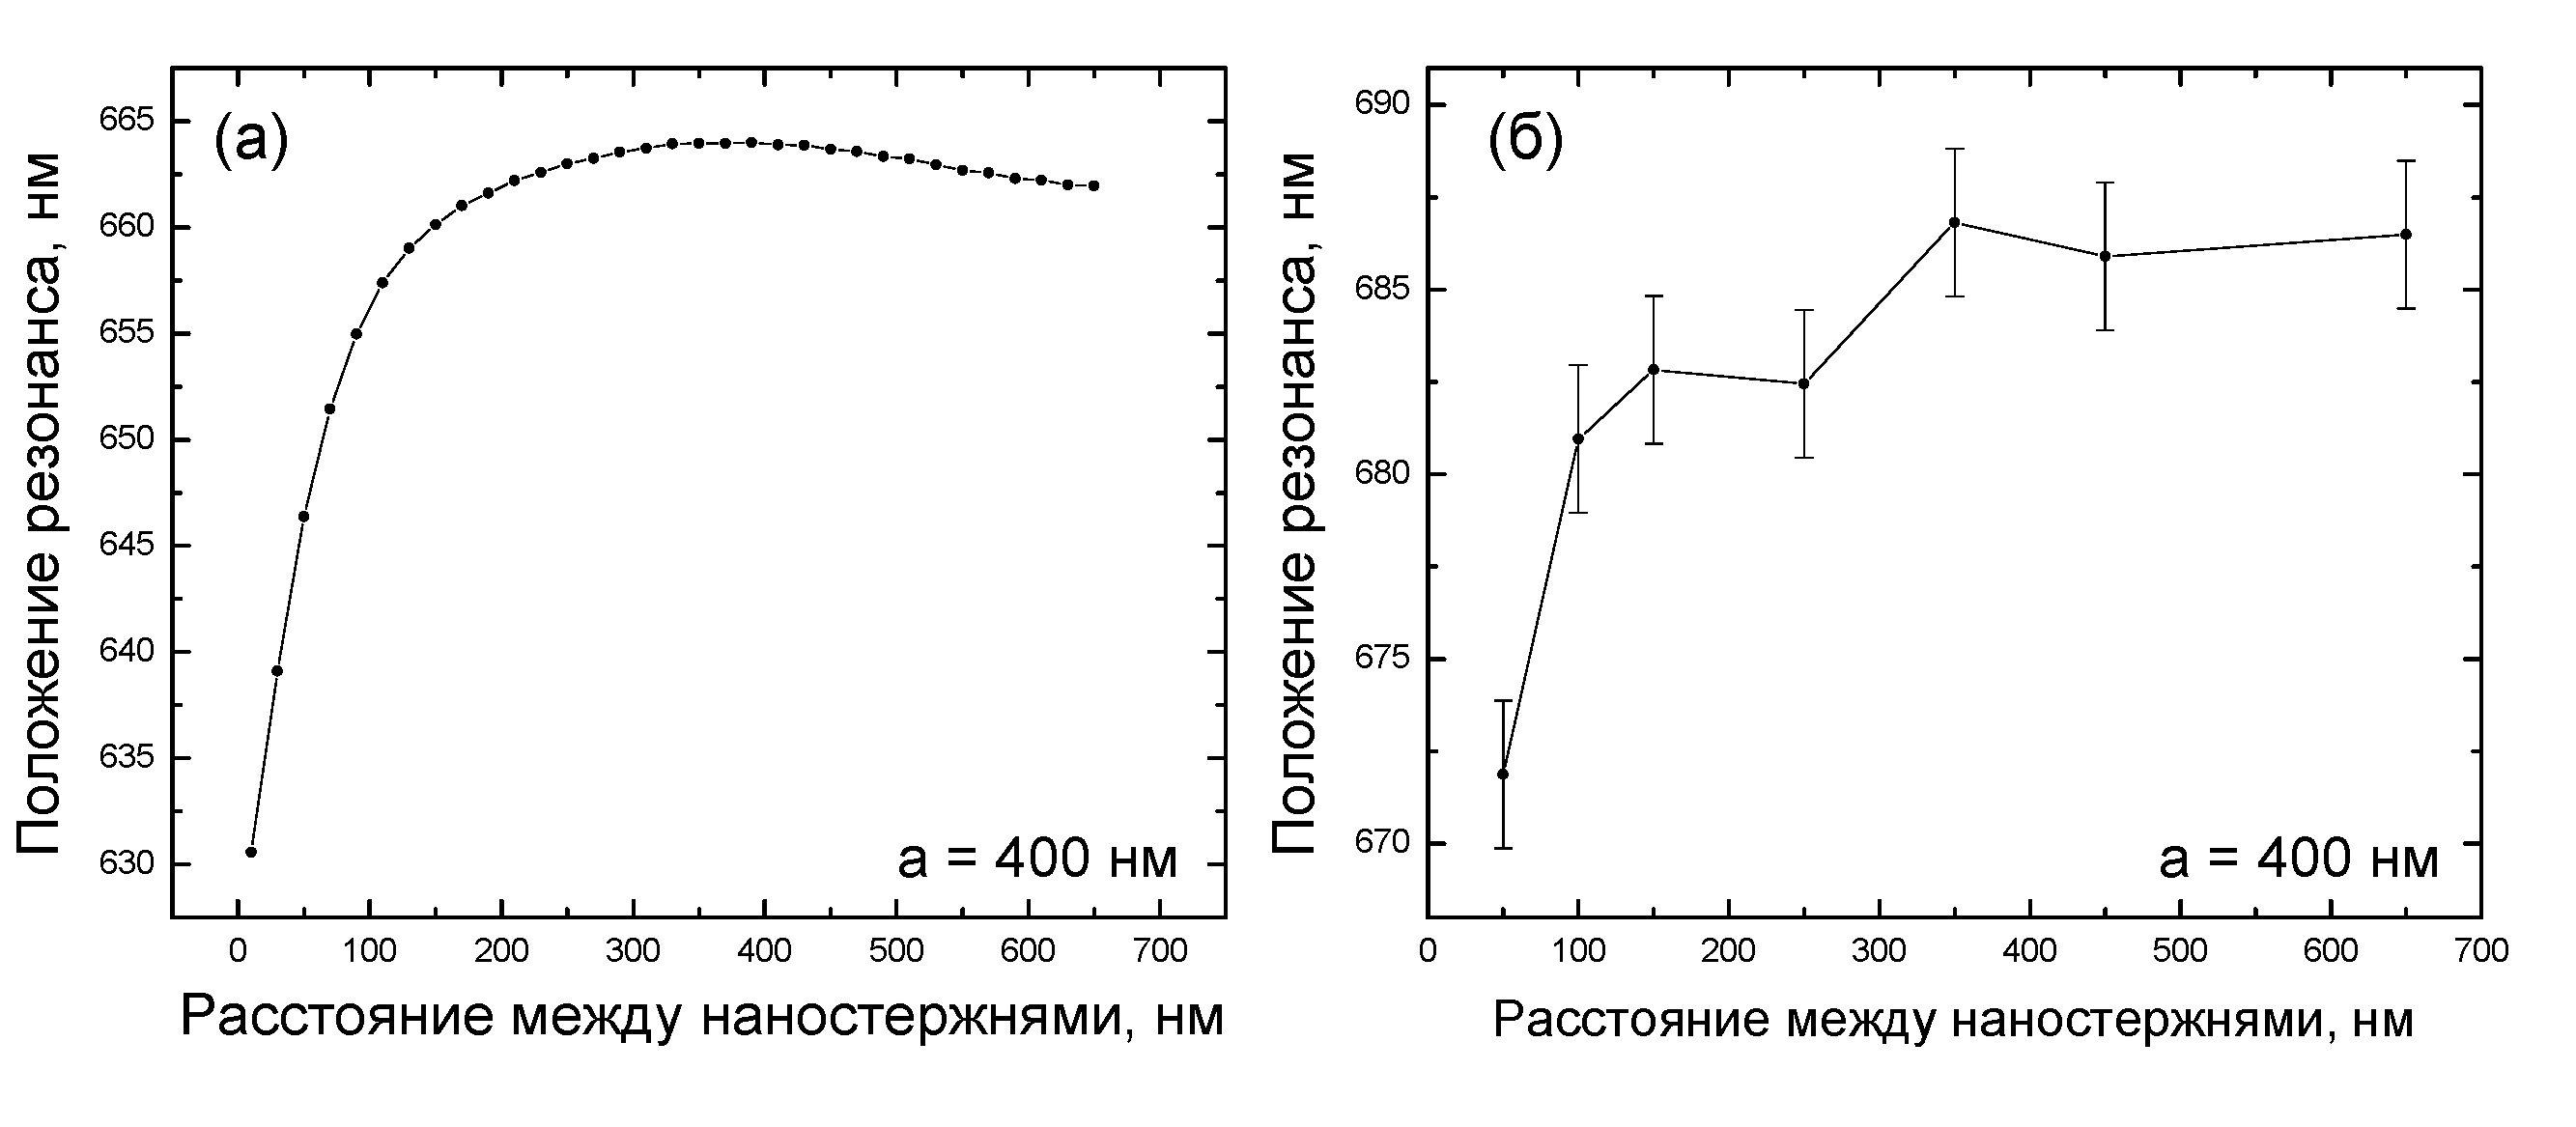
\includegraphics[width=16cm]{img/microspectroscopy/a400simexp.pdf}}
\caption{Рассчитанный численно (а) и полученный экспериментально (б) график зависимости положения резонанса второго порядка от расстояния между наностержнями для длин наностержней 400 нм. }
\label{img:a400simexp}
\end{figure}
\begin{figure}
\center{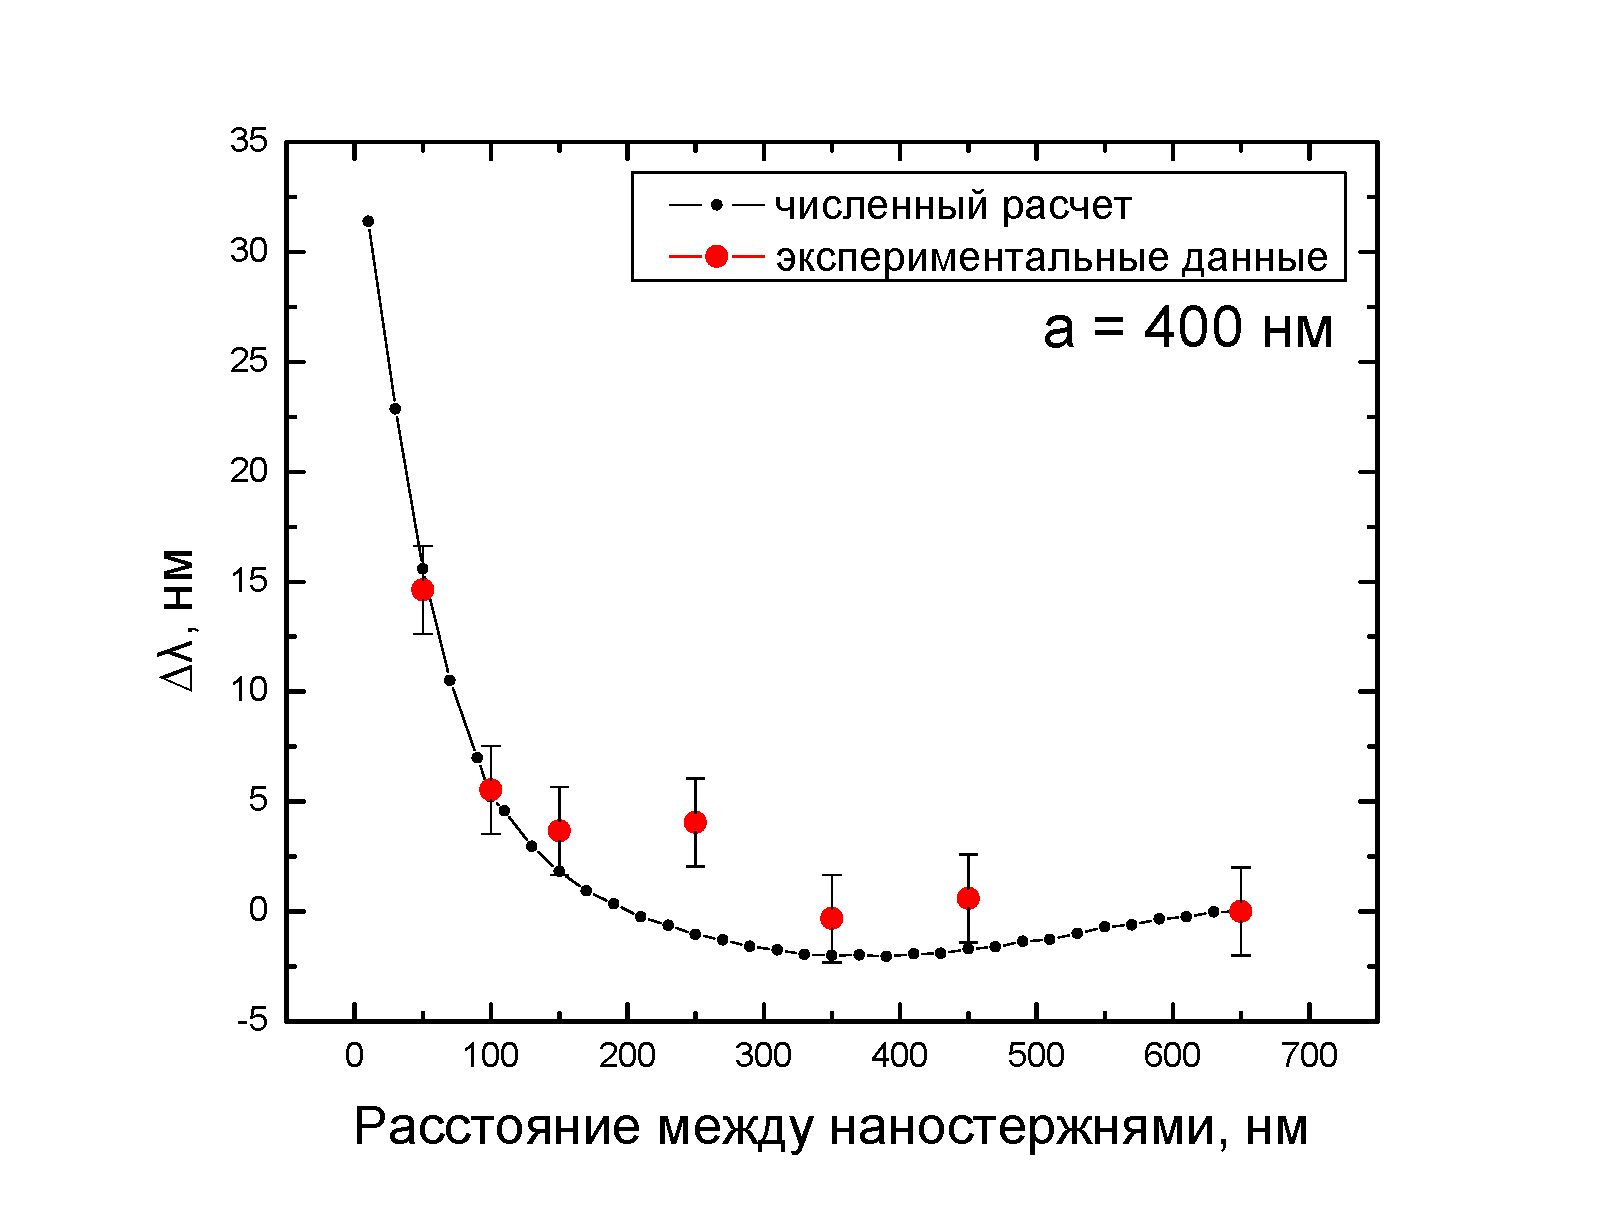
\includegraphics[width=10cm]{img/microspectroscopy/a400shift.pdf}}
\caption{График относительного сдвига резонанса второго порядка от расстояния между наностержнями при длине наностержней 400 нм.}
\label{img:a400shift}
\end{figure}
Такое поведение резонанса ЛПП хорошо согласуется с исследованиями систем димеров другой геометрической формы \cite{plasonrulereq, nanoprism}.

Далее исследовался спектр пропускания димеров с длиной 100, 150 и 200 нм. Характерный спектр пропускания для наностержней длиной 150 нм и расстоянием между наностержнями 100 нм показан на рис.~\ref{img:Spectraa1d1}. Глубина модуляции резонанса ЛПП составляет примерно 10 \%, а ширина на полувысоте резонанса ЛПП --- 100 нм. Для длин наностержней 150 нм данный резонанс является резонансом первого порядка.
\begin{figure}
\center{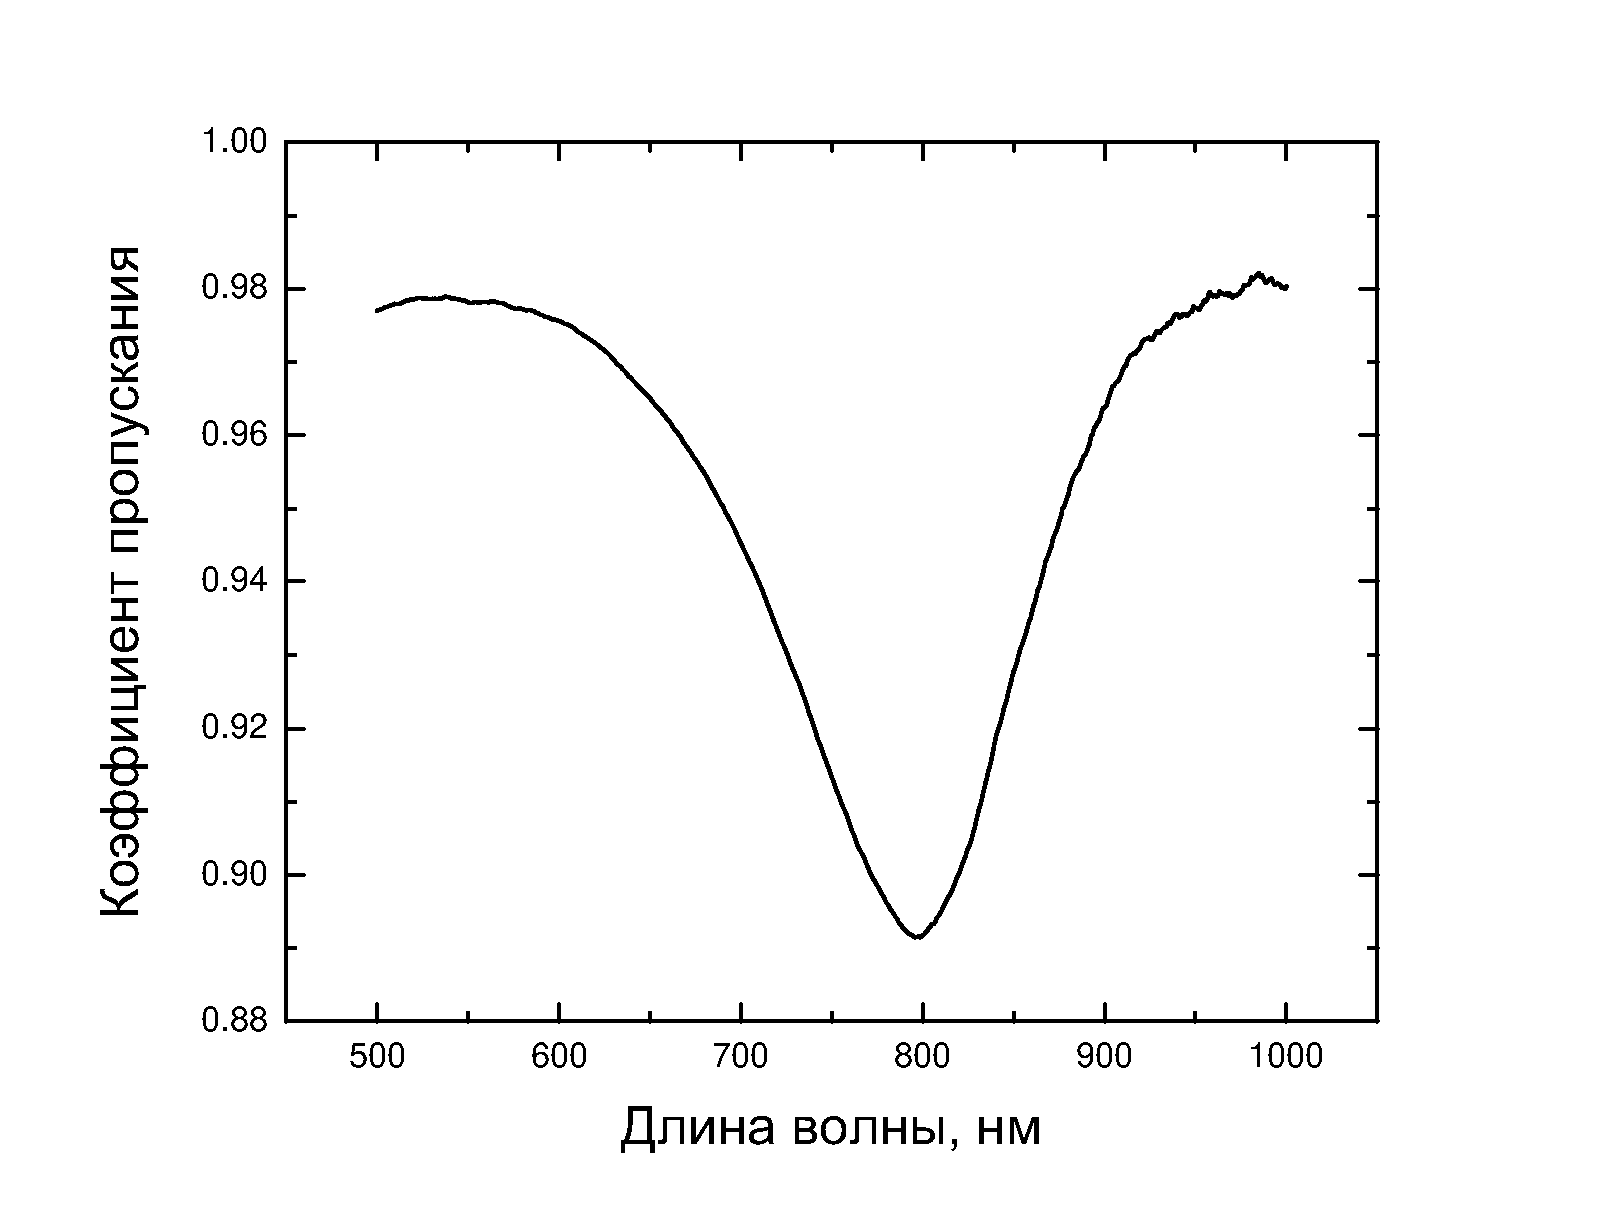
\includegraphics[width=10cm]{img/microspectroscopy/a150d100_spectra.pdf}}
\caption{Спектр пропускания ансамбля из наностержней с длиной 150 нм и расстоянием 100 нм между ними.}
\label{img:Spectraa1d1}
\end{figure}

На рис.~\ref{img:1res} показана зависимость резонанса первого порядка от расстояния между наностержней для длин наностержней 100, 150, 200 нм. Зависимость не носит характера насыщения, и наблюдаются осцилляции резонанса ЛПП первого порядка. Это связано, скорее всего, с дальнепольным взаимодействием наностержней, а также дифракционным взаимодействием между димерами, расстояние между которыми $ \approx 1$ мкм. Данные осцилляции являются паразитными для задачи построения <<плазмонной линейки>>, поскольку они мешают построению калибровочной кривой. Таким образом из экспериментальных данных следует, что для резонанса второго порядка возможно построить <<плазмонную линейку>> из-за его слабой чувствительности к дальнепольному взаимодействию, а для резонанса первого порядка влияние дальнопольного взаимодействия приводят к невозможности построения <<плазмонной линейки>>.
\begin{figure}
\center{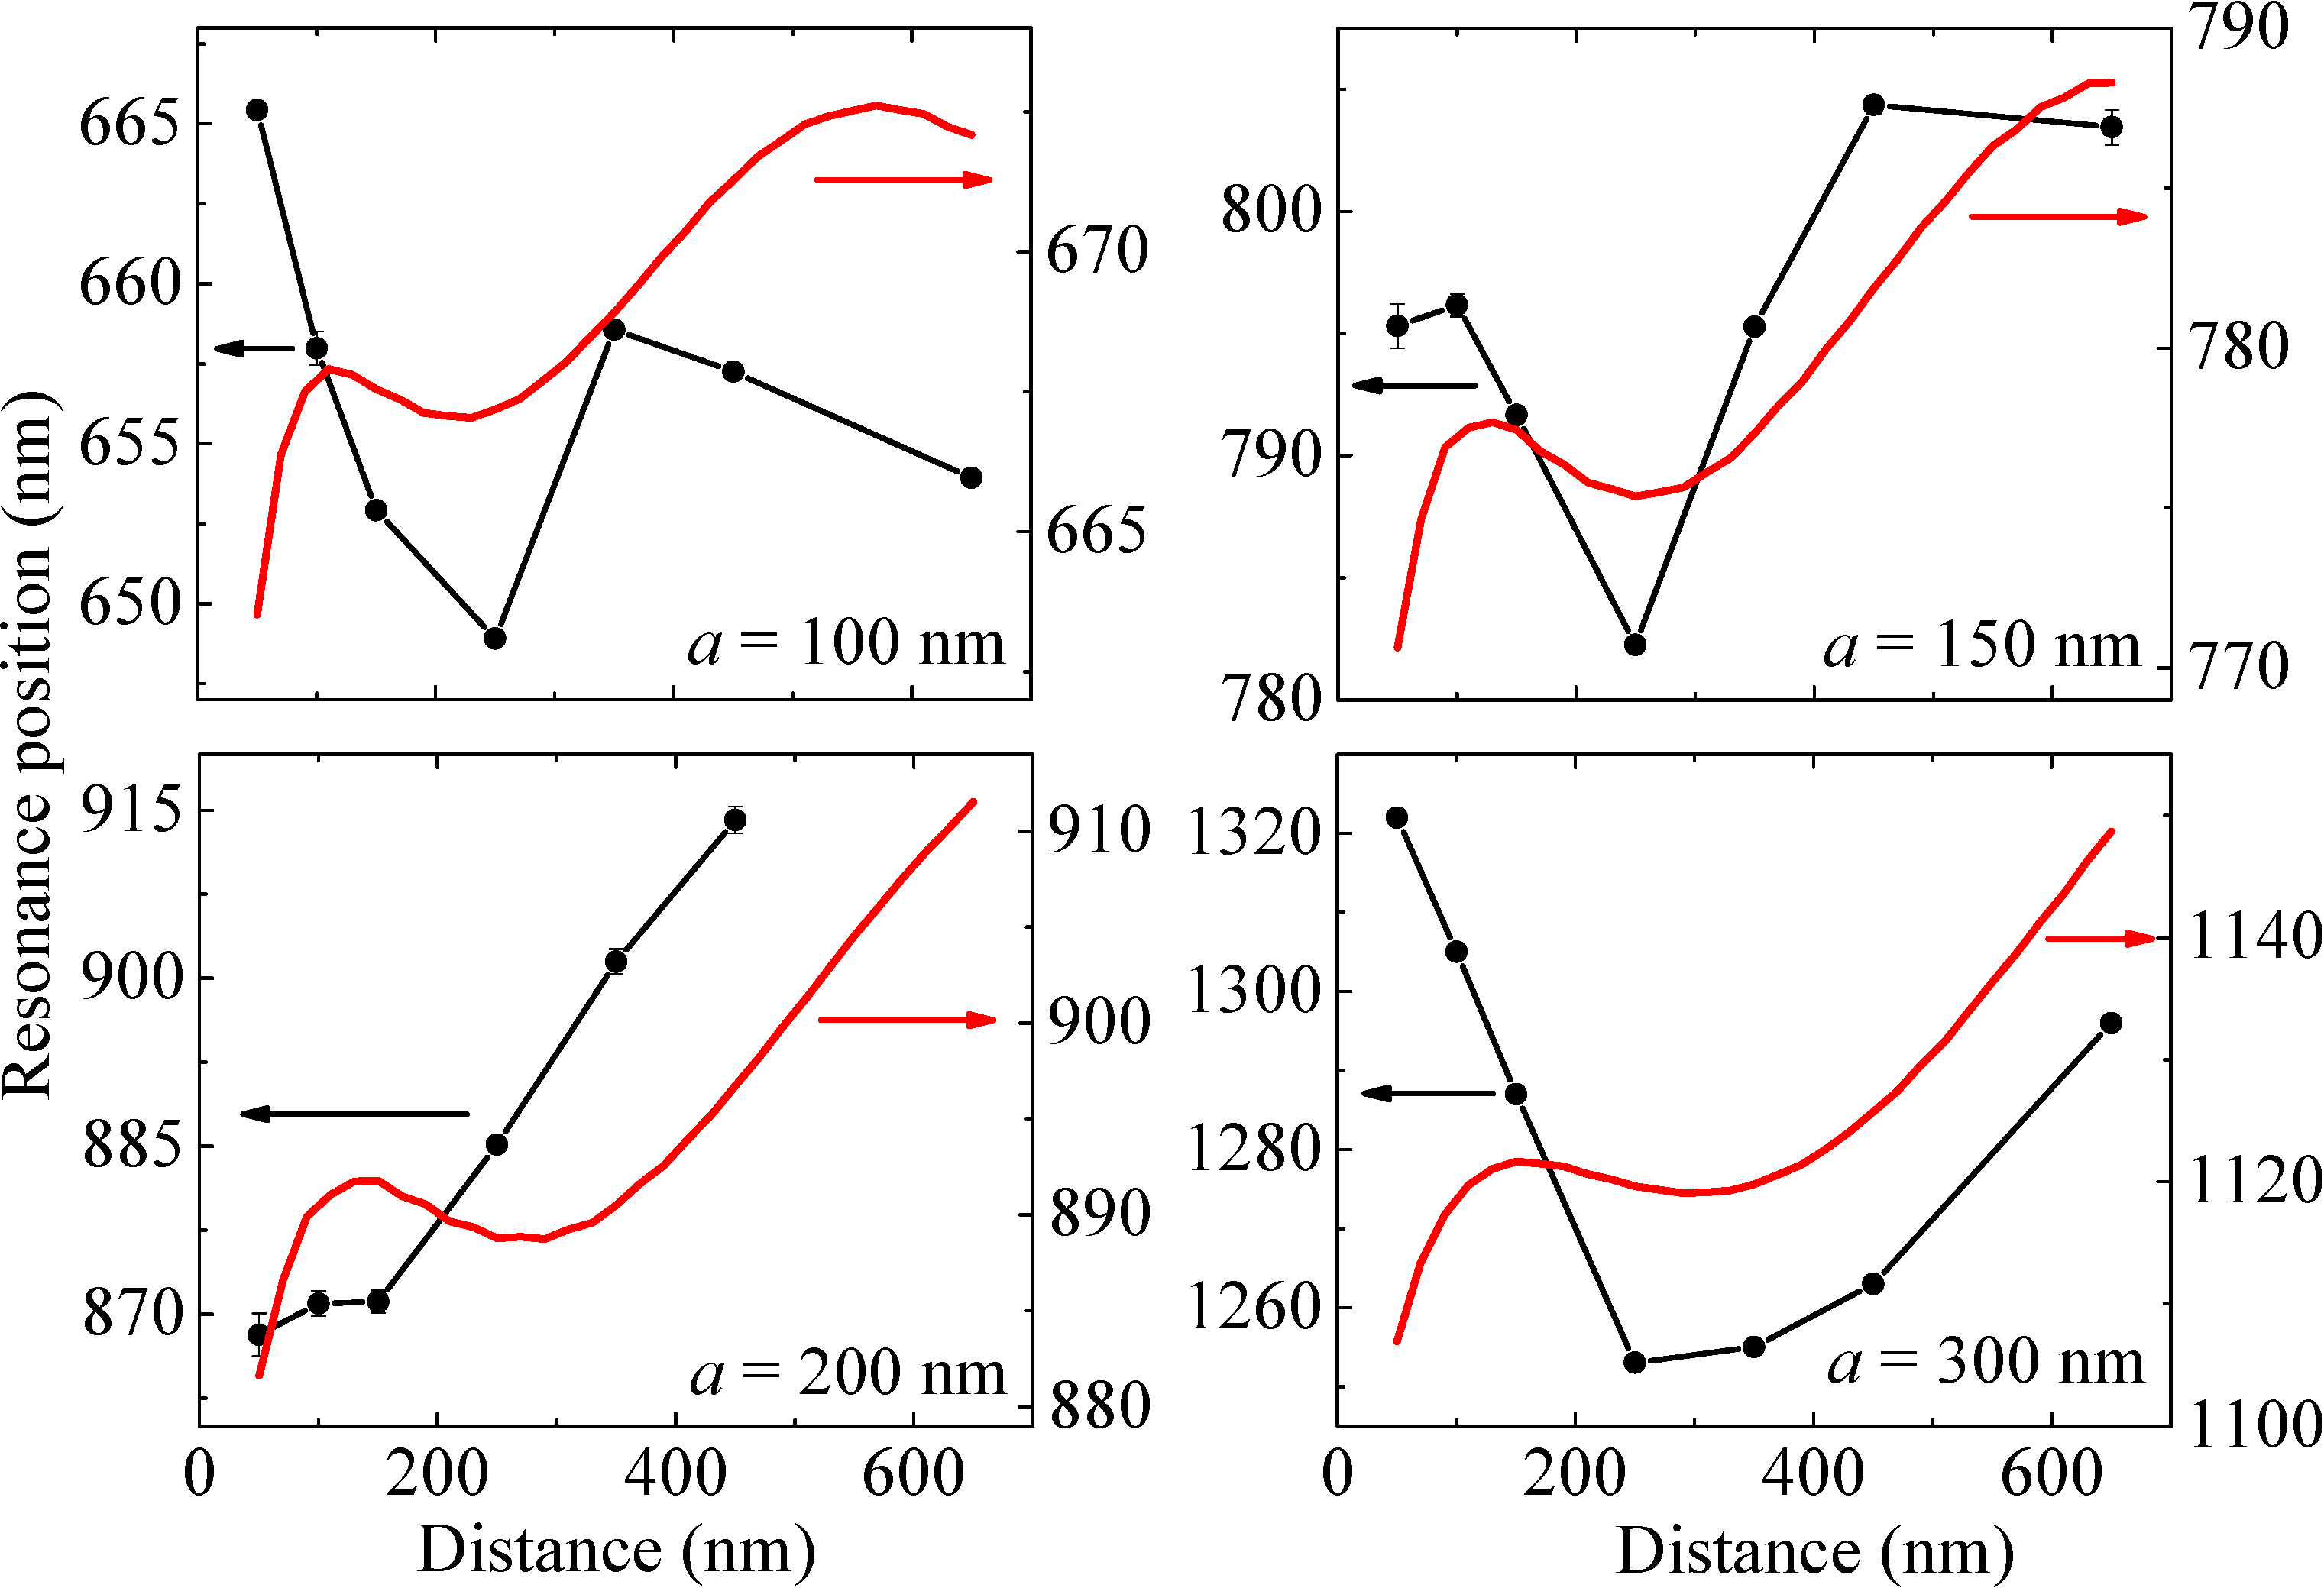
\includegraphics[width=18cm]{img/microspectroscopy/1res.pdf}}
\caption{Зависимость положения резонанса ЛПП первого порядка от расстояния между наностержнями при длине наностержней 100 нм, 150 нм и 200 нм.}
\label{img:1res}
\end{figure}


\section{Аналитический расчет взаимодействия двух диполей с резонансной поляризуемостью}
Рассмотрим взаимодействие двух диполей без приближения ближнего поля (\ref{eq:f_Taylor}). Так как поляризация первого диполя создает электрическое поле в первом диполе, а поляризация второго диполя --- в первом, и зная соотношение между электрическим полем $ \textbf{E} (r) $ и поляризацией $ \textbf{P} $ из формулы (\ref{eq:elecdipole}) и введя коэффициент $ \beta $, получим системы линейных однородных алгебраических уравнений относительно поляризации $ \textbf{P} (i) $, где $ i $ --- i-ый диполь:
\begin{subequations}
\begin{gather}
\frac{\mathbf{P}(1)}{\alpha} - \beta \mathbf{P}(2) = 0, \label{eq:linear_eq_P1} \\
\beta \mathbf{P}(1) -  \frac{\mathbf{P}(2)}{\alpha} = 0, \label{eq:linear_eq_P2} 
\end{gather}
\end{subequations}
где $ \alpha $ --- поляризуемость, определяемая формулой (\ref{eq:polarizability_dipole}), а произведение $ \beta \textbf{P} $ определяется в общем случае формулой
\begin{multline}
\beta \mathbf{P} = \exp (\imath k r) \Bigg( \Bigg[ \frac{P_x}{r} \left( k^2 + \imath \frac{k}{r} - \frac{1}{r^2} \right) \Bigg] \mathbf{e_x} + \Bigg[ \frac{P_y}{r} \left( k^2 + \imath \frac{k}{r} - \frac{1}{r^2} \right) \Bigg] \mathbf{e_y} + \\
+ \Bigg[ \frac{P_z}{r} \left( - \imath \frac{2 k}{r} + \frac{2}{r^2} \right) \Bigg] \mathbf{e_z} \Bigg).
\label{eq:2D_susceptibility}
\end{multline}
Рассмотрим анизотропный тензор поляризуемости $ \alpha_{ij} = 0 $, кроме $ \alpha_{xx} \neq 0 $. Тогда в уравнении (\ref{eq:2D_susceptibility}) не равны нулю только коэффициенты при $ \mathbf{e_x} $. Представим систему уравнений (\ref{eq:linear_eq_P1}, \ref{eq:linear_eq_P2}) в виде матрицы и найдем через ее собственные значения резонансные частоты $ \omega_s $ и $ \omega_a $, которые относятся к симметричному и антисимметричному случаю взаимодействия диполей. В ходе анализа был написан скрипт в программном пакете MATHEMATICA, который вычислял положения резонансов $ \lambda_s $ и $ \lambda_a $. Далее была исследована зависимость положения резонансных длин волн $ \lambda_s $ и $ \lambda_a $ от расстояния между диполями. Для этого выбирались определенное расстояние $ d $ между диполями от значения $ d = $ 50 нм до $ d = $ 400 нм с шагом 1 нм и численно находились резонансные длины волн  $ \lambda_s $ и $ \lambda_a $. На рис.~\ref{img:2D_res} показана зависимость положения резонанснов ЛПП $ \lambda_s $ и $ \lambda_a $ от расстояния между диполями. Видно, что в отличие от зависимости в ближнепольном приближении (рис.~\ref{img:semianalytical_dd}) появляются осцилляции, связанные с влиянием дальнего поля.
\begin{figure}
\center{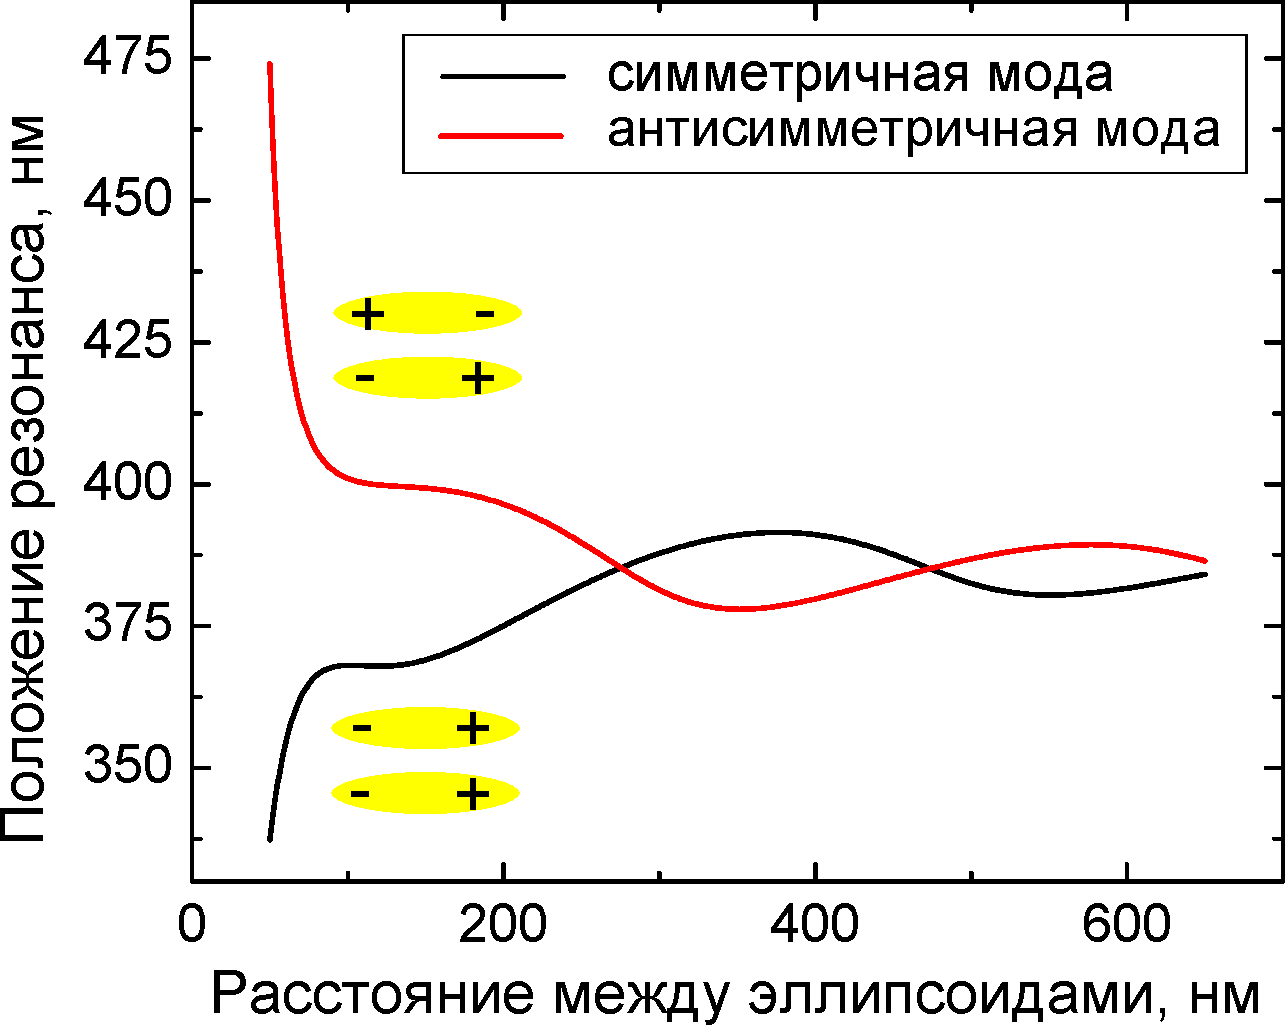
\includegraphics[width=0.5\linewidth]{img/analytics/res_dd.pdf}}
\caption{Зависимость положения симметричного $ \lambda_s $ и антисимметричного $ \lambda_a $ резонанса от расстояния $ d $ между диполями. Вставки --- мгновенное распределение зарядов в случае симметричной и антисимметричной моды.}
\label{img:2D_res}
\end{figure}
Данные осцилляции являются <<паразитными>> для верхней границы применимости димера в качестве плазмонной линейки. Они связаны с тем, что в отличие от формулы (\ref{eq:wl_dipole}), в которой учитывалась только ближнепольная компонента поля $ \frac{1}{r^2} $, учитывается и влияние множителей $ \frac{k}{r} $ , $ k^2 $, а экспонента не раскладывается в ряд Тейлора по малому параметру $ kr $.

%Абзац -- сравнение аналитического решения и численного расчета FDTD
Далее рассматривались эллипсоиды различной длины. По формуле (\ref{eq:Lfactor}) рассчитывался фактор деполяризации данного эллипсоида, а по формуле (\ref{eq:polarizabilityEllip}) --- его поляризуемость. Для эллипсоидов с длиной $ a = $ 100, 150, 200 и 300 нм рассчитывалась зависимость положения резонансной длины волны ЛПП симметричной моды от расстояния между эллипсоидами. Полученные данные сравнивались с численными расчетами для $ \pi $-димера золотых наностержней такой же длины с граничными условиями PML на рис.~\ref{img:res1_analytic_FDTD}.
\begin{figure}[t]
\center{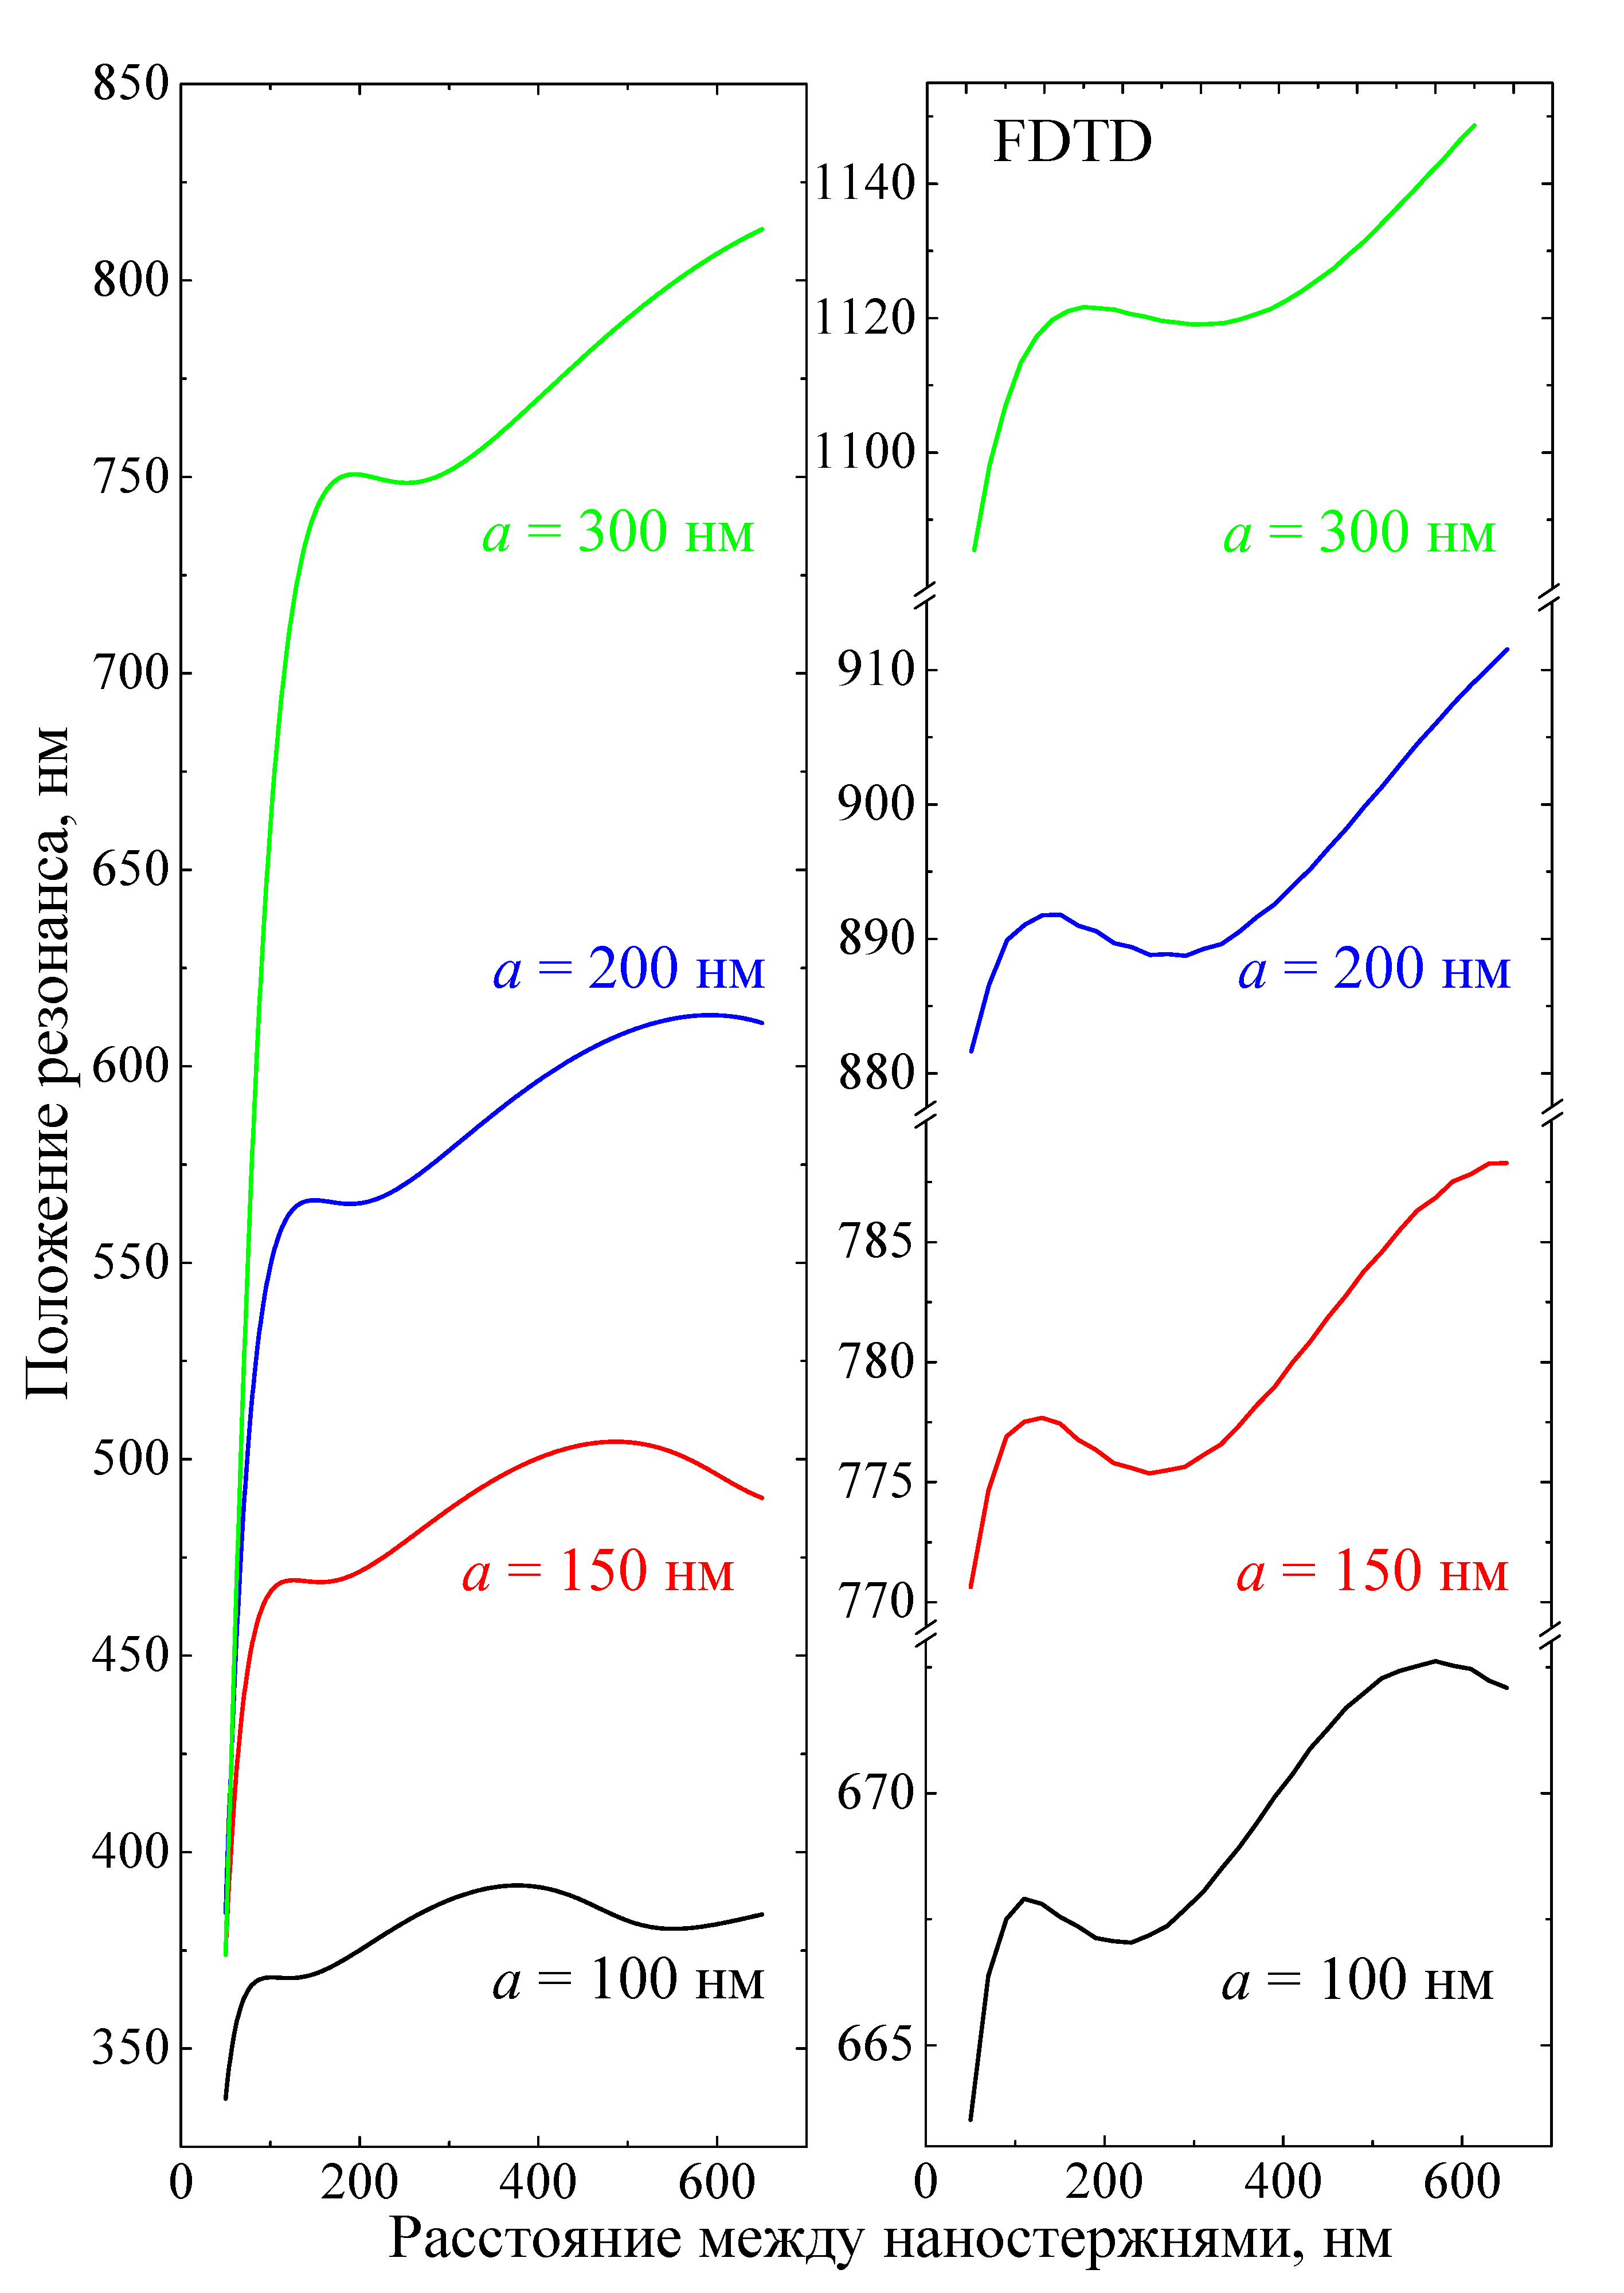
\includegraphics[width=0.6\linewidth]{img/analytics/res1_analytic_FDTD.pdf}}
\caption{Зависимость положения резонансной длины волны ЛПП $ \lambda_s $ от расстояния между наностержнями с длиной $ a = $ 100, 150, 200, 300 нм.}
\label{img:res1_analytic_FDTD}
\end{figure}
Как в аналитических, так и в численных расчетах наблюдаются осцилляции. Эти осцилляции связаны дальнепольным взаимодействием эллипсоидов. Кроме того, период этих осцилляций увеличивается с увеличением длины эллипсоидов в случае аналитического расчета и с увеличением длины наностержней в случае численного расчета. 
\section{Обсуждение результатов}

Рабочим диапазоном плазмонной линейки в данной работе является расстояние между наностержнями от $ d = $ 0 нм до такого значения резонанса ЛПП $ \lambda_0 (d)$, при котором производная $ \lambda'_0 (d) $  в первый раз равняется нулю. Из численных результатов (рис.~\ref{img:res_comparison}) было получено, что верхняя граница применимости <<плазмонной линейки>> в случае резонанса первого порядка составляет $ \approx 170 \pm 10 $ нм, а в случае резонанса второго порядка она больше и составляет $ \approx 370 \pm 10 $ нм. Из экспериментальных данных мы видим, что для резонанса ЛПП второго порядка экспериментальная кривая положения резонанса ЛПП от расстояния между наностержнями согласуется с численными расчетами за исключением того, что в абсолютных значениях экспериментально полученные данные положения резонанса ЛПП сдвинуты в красную область на  $ \approx 25 $ нм в случае длины наностержней $ a = $ 400 нм и на $ \approx 50 $ нм в случае длины наностержней $ a = $ 500 нм. Это связано с тем, что численном расчете не учитывалась кварцевая подложка, которая влияет на положение резонанса ЛПП. В случае резонанса первого порядка ЛПП экспериментальные данные не согласуются с численными расчетами (рис.~\ref{img:1res}). Это связано с дифракцией между $ \pi $-димерами в исследуемых образцах, так как проводилась микроспектроскопия спектроскопия пропускания ансамбля одинаковых $ \pi $-димеров, а не одиночного $ \pi $-димера. В случае же численного эксперимента при расчете зависимости положения резонанса ЛПП от расстояния между наностержнями использовались граничные условия PML, которые с физической точки зрения поглощают все падающее на них электромагнитное поле. Для того, чтобы учесть периодичность структуры в были проведены численные расчеты спектров коэффициента экстинкции для $ \pi $-димеров с фиксированной длиной наностержней $ a = $ 300 нм и расстоянием между наностержней $ d = $ 300 нм от расстояния между $ \pi $-димерами (рис.~\ref{img:BCperiod}). Для этого граничные условия PML были изменены на периодические граничные условия. Видно, что резонанс второго порядка менее чувствителен к периоду между $ \pi $-димерами, в то время как положение резонанса первого порядка начинает сильно варьироваться из-за дифракционного взаимодействия между $ \pi $-димерами, а иногда происходит расщепление резонанса ЛПП. Аналогичный эффект дифракционного взаимодействия наблюдался в случае периодически расположенных наноантенн в статье \cite{diffractionCoupling}. Наноантенны представляли из себя нанокольца и наблюдалось два резонанса: дипольный и квадрупольный. В итоге квадрупольный резонанс оказался менее чувствителен к дифракционному взаимодействия наноантенн.
Таким образом, дифракционное взаимодействие $ \pi $-димеров и дальнепольное взаимодействие между наностержнями в димере приводят к тому, что верхняя граница применимости $ \pi $-димера в случае резонанса первого порядка меньше, чем для резонанса второго порядка. 
\nonumchapter{Выводы}

Основные выводы могут быть сформулированы следующим образом:
\begin{enumerate}
\item Построена аналитическая модель смещения резонанса локальных плазмон-поляритонов в димерах золотых наностержней.  В качестве модели использовалось взаимодействие двух точечных диполей, диэлектрическая проницаемость которых описывается формулой Друде. Была получена аналитическая формула зависимости резонанса локальных плазмон-поляритонов от расстояния между наностержнями, а также показано существование двух мод: симметричной и антисимметричной.
\item Численно исследовано методом конечных разностей во временной области  смещение резонанса локальных плазмон-поляритонов в димерах золотых наностержней. В ходе исследования было обнаружено наличие двух резонансов локальных плазмон-поляритонов с различным локальным распределением плотности мощности электромагнитного поля для наностержней длиной до 500 нм. На основе смещения положения резонансов первого и второго порядков были получены уравнения для <<плазмонных линеек>>.
\item Получена верхняя граница возможности использования рассматриваемых димеров золотых наностержней в качестве <<плазмонной линейки>>. Для резонанса первого порядка она составляет $  150 \pm 10 $ нм, а для резонанса второго порядка --- $ 400 \pm 30 $ нм.
\item Методами микроспектроскопии пропускания экспериментально охарактеризованы смещения резонанса локальных плазмон-поляритонов.  При этом для длин наностержней 100, 150 и 200 нм наблюдался резонанс первого порядка, а для наностержней длиной 400 и 500 нм --- резонанс второго порядка. Экспериментальные данные смещения резонанса второго порядка сходятся в пределах погрешности с результатами численного расчета, что говорит о возможности использования данной системы в качестве <<плазмонной линейки>>.

\end{enumerate}
%\newpage

\bibliography{mybib}

\end{document}